%% Except where otherwise indicated this code was originally written
%% by, and continues to be maintained by, Marcel Oliver. It is released
%% into the public domain. 
%% Where otherwise indicated, code is covered by the licensing terms of
%% the original packages.
%% The above statement was added 2009/01/05 by Clea F. Rees on behalf 
%% of the author.
% \iffalse
%%
%% File ua-classes.dtx by Marcel Oliver
%%
%% Documentation can be obtained by running "latex labels.dtx"
%%
%<*dtx>
\ProvidesFile{ua-classes.dtx}
%</dtx>
%<driver>\ProvidesFile{ua-classes.drv}
%
%<*driver>
\documentclass{ltxdoc}
\begin{document}
\DocInput{ua-classes.dtx}
\end{document}
%</driver>
% \fi
%
% \title{Document Classes for \\
%        Writing Theses and Dissertations \\
%        for Submission at the University of Arizona}
% \author{Marcel Oliver}
% \date{1996/05/09}
% \maketitle
%
% \begin{abstract}
% This package provides a \LaTeXe\ document class named |ua-thesis|
% for typesetting theses and dissertations in the official format required
% by the University of Arizona.  
% Moreover, there is a fully compatible alternative document class
% |my-thesis| for private copies of the dissertation, and the respective
% title pages are available as separate packages to work with ``any''
% document class.  
% \end{abstract}
% 
%
% \section{User Documentation}
%
% \subsection{Introduction}
%
% The |ua-thesis| document class is designed to conform with the official
% requirements of the Graduate College of the University of Arizona.  It is
% based on the |report| class which comes with the standard \LaTeX\
% distribution, and all commands are upward compatible with |report|
% and to a large extend with the |amsbook| class.  In other words, any
% document which works error free in those two classes should run with
% |ua-thesis|, too.  To automatically typeset all the required information,
% a few new commands are defined, which are explained below.
%
%
% \subsection{Classes and Options}
%
% The following classes and packages are provided:
%
% \begin{description}
%
% \item[\texttt{ua-thesis}]
% The official University of Arizona thesis document class.  The |draft|
% option is a paper saver---the automatic generation of front matter pages
% other than the title page will be suppressed, and single spaced printing
% will be used throughout the document.  The |final| option activates
% ``double spaced'' layout at the required places and creates the full set
% of front matter pages.  The default is |draft|. 
%
% Note that the draft option is passed through to the underlying |report|
% class, i.e.\ thick black rules will indicate the location of overfull
% |hbox|es.
%
% The |ua-thesis| class automatically loads the |amsmath|, |amssymb| and
% |amsthm| packages which considerably improve the mathematical
% typesetting capabilities of \LaTeX.  The use of these macros is strongly
% recommended. 
%
% The default type-size in this document class is 12pt and should not be
% changed.  Subsubsections 
% produce unnumbered run-in headings which do not appear in the Table of
% Contents, therefore their use is discouraged.
%
% \item[\texttt{my-thesis}]
% An alternative to |ua-thesis| to produce private copies of your
% dissertation which don't look so reminiscent of the typewriter age.  It
% is based on the |pcms-l| document class by the American Mathematical
% Society, which was designed to typeset monographs for the Park City/IAS
% Mathematics Series.  It is similar to |amsbook|, but has a less crowded
% look.
%
% \item[\texttt{ua-title}]
% The official University of Arizona title page as a separate package.
% Useful if you want to build your own private thesis class, but want to
% use the official title page.  It redefines the |\maketitle| command and
% also provides (potentially useless) definitions for all the commands
% described in the next section.
%
% The package is neither guaranteed nor tested to work with any specific
% document class.  You have to try and see.
%
% \item[\texttt{my-title}]
% The equivalent to |ua-title|, but with the title page of the |my-thesis|
% class. 
% 
% \end{description}
% So, the first line in your dissertation file should be
% \begin{verbatim}
%   \documentclass{ua-thesis}
% \end{verbatim}
% or, for the final printout,
% \begin{verbatim}
%   \documentclass[final]{ua-thesis}
% \end{verbatim}
% If you change the document class from |ua-thesis| to |my-thesis| or vice
% versa, the 
% first \LaTeX\ run might produce error messages because the format of the
% auxiliary files (|.aux|, |.toc| etc.) is incompatible between the two.
% Type |s| or |q| to ignore all error messages and run \LaTeX\ a second
% time, or manually delete all auxiliary  
% files before changing the document class.
% 
%
% \subsection{Commands for Specifying the Front Matter}
%
% As in the standard document classes, the title of your thesis is
% specified by
% \begin{verbatim}
%   \title{This is the Title of my Dissertation \\
%          and This is the Second Line}
% \end{verbatim}
% where line breaks can be forced with |\\| if the automatic line
% breaking does not give a satisfactory result.  But remember, the Graduate
% College imposes a maximum of three lines in the title---\LaTeX\ does not
% check this for you.  An optional argument can be given for reasons of
% compatibility with the AMS classes, but will be ignored.
%
% Your name is specified with
% \begin{verbatim}
%   \author{Firstname Lastname}
% \end{verbatim}
% again, an optional argument will be ignored.  Use
% \begin{verbatim}
%   \date{1996}
% \end{verbatim}
% set the year of your graduation.  If you omit this command, the current
% day, month and year will be printed, which may be useful for keeping
% track of different draft versions.
% The only other command that is required for the final version of every
% dissertation is 
% \begin{verbatim}
%   \director{Firstname Lastname}
% \end{verbatim}
% to specify the name of your dissertation advisor.  It will appear on the
% Special Abstract which is automatically generated.  
%
% Now the optional commands. The name of your department is set with
% \begin{verbatim}
%   \department{Department of Metaphysics}
% \end{verbatim}
% The default is ``Graduate Interdisciplinary Program in Applied
% Mathematics''. If you are in the ``Department of Metaphysics'', you have
% to use this command.
%
% If you are writing a Masters thesis, you have to explicitly specify the
% name of your degree.  Use
% \begin{verbatim}
%   \degree{Masters of Arts}
% \end{verbatim}
% The default is ``Doctor of Philosophy''.  The abbreviation of the
% degree is needed for the Special Abstract and can be with
% \begin{verbatim}
%   \degreeabbrev{M.A.}
% \end{verbatim}
% The default is ``Ph.D.''.  Moreover, for Masters theses, the Copyright
% Page will have an additional part for the approval signature of your
% advisor.  It will be automatically generated whenever you specify your
% advisor's title with
% \begin{verbatim}
%   \directortitle{Professor of Mathematics}
% \end{verbatim}
% The default is empty and \emph{must not be changed for doctoral
% dissertations}. 
%
% If you have to specify a major department
% different from the department above, use
% \begin{verbatim}
%   \major{Agriculture}
% \end{verbatim}
% The default is empty.  
%
% You can copyright your dissertation or thesis by writing
% \begin{verbatim}
%   \copyrightholder{Firstname Lastname Year}
% \end{verbatim}
% The default is empty.  If you use this command, the 
% Copyright Page will automatically change to the required
% legalese for copyrighted dissertations or theses.
% 
%
% \subsection{Examples for the Root File}
%
% For long documents such as theses, it is useful to split the \LaTeX\
% source code into several files.  The root file is the file that you run
% \LaTeX\ on.  Subordinate files are included with |\include|.
%
% \subsubsection{A Doctoral Dissertation}
%
% The example below also shows how to load the |graphics| package, which in
% particular supports the inclusion of postscript images.  Note that you
% can specify the |draft| or |final| option for the graphics package
% separate from the global options of the document class.
%
% The |ua-thesis| class is designed to create a |.dvi| file that strictly
% adheres to the required page margins.   The printer hardware or the
% driver implementation, however, may have tolerances that cause the image
% to shift on the page.  This can be corrected by using |\hoffset|
% and |\voffset|.  The example below works well with the current printers
% in the Math Department.
%
% You don't need to use |\chapter*{Dedication}| for the Dedication if you
% don't like the heading.  You can simply start a new page with |\newpage|,
% but then you are completely responsible for the formatting of that page,
% including the switch to double-spaced printing as is officially required
% (this can be done, for example, by using |\doublespaced|).
%
% \begin{verbatim}
% \documentclass[draft]{ua-thesis}
% \usepackage[final]{graphics}
%
% \hoffset -2.1mm
%
% \director{Advisor's Name}
% \date{1996}
%
% \title{This is a Doctoral Dissertation}
% \author{Your Name}
%
% \begin{document}
%
% \maketitle
%
% \chapter*{Acknowledgments}
% Acknowledgments go here.
%
% \chapter*{Dedication}
% Dedicated to the Fundamental Theorem of Calculus.
%
% \tableofcontents
% \listoffigures
% \listoftables
%
% \begin{abstract}
% This is the abstract. 
% \end{abstract}
%
% %!TEX root = ../Dissertation_RC.tex
%\makeatletter
%\providecommand*{\input@path}{}
%\g@addto@macro\input@path{{../}{../../}}% append
%\makeatother
%\documentclass[../Dissertation_RC.tex]{subfiles}
%
%\begin{document}
\chapter{Introduction}
	\section{Introduction}
		\label{intro}
%A good introduction answers some of these questions:
%\begin{enumerate}
%	\item What does this paper talk about?
%	\item What makes it interesting?
%	\item Why is it important?
%	\item What is the context for the problem?
%	\item How will will measure the progress (at least here?)
%	\item Where did the inspiration come from?
%	\item What is(are) original contribution(s)?
%\end{enumerate}
%
%
%The introduction describes the area in which you are working, gives the basic definition
%and terminology, and sets out the fundamental results. If your dissertation contains a proof
%of a result, which may be yours or someone else’s, then you should give the statement of the
%result in the introduction and explain its significance.
%
%As a good rule for structuring any argument, in particular the introduction, it is useful
%to answer the sequence of questions what – why – how. Always state what you are talking
%about first before justifying it or diving into details.
%
%The “what” part of the introduction summarises the contents of your dissertation. Ideally,
%you should be as informative as possible. Obviously you cannot say everything at once, so
%you may have to simplify. You may choose to tell a “white lie”, but you should try not to
%make statements that are wrong; for instance, you may by add a qualifier like “under certain
%reasonable assumptions”.
%
%The introduction should always cite and, if possible, summarise relevant work done by
%others. This puts the work of the dissertation in context and allows the reader to judge the
%dissertation’s contribution. If you can do so briefly, you may give a history of your subject
%first in order to explain what the current work is about. In that way, you simultaneously take
%care of the “what” and the “why” part.
%
%Usually, the “what” part comes first, the “why” at a suitable time later. The “how” part
%should summarise the methods used in the dissertation, and possibly give further details.
%If you present original research, it is good to explain the main ideas in the introduction,
%and make them sound as un-mysterious as possible. If this is done well in the introduction,
%the reader will be curious to read more about them. You should make it clear that you to
%are the first person to have found something (if that is correct), but be careful and modest
%about it.
%
%At any rate, make it clear in the introduction what your own contributions are, which may
%be original research or in terms of exposition. Do not be shy to state contributions that are
%small, for example “in Section 5 we illustrate Theorem X of [Y] with an example”.
%The final paragraph of the introduction is typically a brief list of the sections of the
%dissertation and their contents.
%
%The following is a list of common mistakes in an introduction and how to avoid them.
%\begin{enumerate}
%	\item Exaggerated claims, for example “differential games are one of the most important tools
%	of economics”. This may be your impression after studying differential games, but it
%	sounds naive. Adopt a neutral tone, and remain careful and factual. The subject of the
%	dissertation does not have to be declared as very important.
%	\item Assuming too much knowledge from your reader. You have immersed yourself in the
%	topic for several months, but your reader has not. Be aware of that, and explain and
%	introduce your topic in a comprehensible way.
%	\item An introduction that is an unclear medley of exposition, history of the subject, and a
%	repetition of what others have done. A good way out of this is to deal with these aspects
%	separately, in particular, to postpone the exposition to a main section. State early what
%	you do in the dissertation. Suppose that the dissertation is mostly on a topic covered in
%	paper X. You may choose similar opening sentences as paper X. However, when paper X
%	says “We solve this problem as follows”, do not say “we”, but say instead “This problem
%	is solved in [X] as follows . . . ” and then state how you will explain the results of paper X
%	in a later section of your dissertation.
%\end{enumerate}
%
%In the writing process, the introduction can normally be finished only when the main text
%is complete because only then do you know its contents and structure. For your dissertation,
%try nevertheless to produce a draft introduction early on. You will get practice in writing,
%and gain valuable feedback on your view of the topic from your supervisor

%%%%%%%%%%%%%%%%%%%%%%%% the above must not fully appear in final dissertation!!!! %%%%%%%%%%%%%%%%%

%\section{actual intro}

%% add information about mixture models (pearson etc.) to intro. maybe include a section in backgd.
This dissertation introduces a new type of neural network layer for classification problems which I call responsible softmax.   I will show that both in theory and practice, responsible softmax may be a useful tool for dealing with imbalanced data of many types, especially when the data can be modeled with a mixture model.

Working with imbalanced data is a common problem in machine learning. There are many reasons for this, though a common one is that some classes of data are difficult to obtain. It may also be that the underlying process creating the data is imbalanced. Regardless of the reason, imbalanced data tends to bias classifiers towards the majority classes.  For this reason and others, it is important to address imbalanced data when choosing an algorithm.
% use forward references from the narrative in the introduction. The introduction (including the 
% contributions) should survey the whole paper, and therefore forward reference every important part.

There have been several techniques developed over the years to handle the problem of data imbalance. Each of these algorithms has several pros and cons. Trade offs between accuracy, precision, computation time, and generalization are not easy to balance. For example, Batista et. al. \cite{DataBalancing} use data balancing to level the per class instances either by undersampling the majority classes, or oversampling the minority classes.  While this can fix the inherent bias against minority classes in typical classifiers, it also can hurt generalization by either severely reducing the data available for training or memorizing (overfitting) the minority class. 

Another example is prior re-weighting (or scaling).  This refers to the idea that the output of a neural network may be modified via Bayes' Rule to appropriately adjust the model of the class mixtures to match what is found empirically.  While I cover this idea in more detail in section \ref{sect:commonLayerConfig} there are many tricks and techniques that fall into this category. See Lawrence e.t. al. \citep{Lawrence2012} for a partial review.
% Mention Focal loss or label smoothing (label smoothing paper?) or place it later?

A final example I give for now is mixture of experts (MOE) \cite{MOEJacobs}. The idea here is to train several learners so that they can differentiate between only a few classes.  The idea here is that each learner could be an `expert' in identifying one or two classes.  Then each expert learner reports their confidence on classification to a gating network.  This gating network is trained to choose the correct expert for each data point. Nets that work as MOE are very adaptable, but they can be expensive to train.  Further, many of the training methods for MOE can get stuck in suboptimal local minima as per Makkuva et. al. \cite{MOEGridlock}.
% I probably need to put most of what i write in the intro later in the dissertation (usually ch 2, but maybe elsewhere?)

Responsible Softmax (RS) addresses some of the problems of imbalance. RS resembles both MOE and prior scaling.  It is similar to prior scaling in that it can be viewed as a re-weighting or regularization of standard softmax layer and cross-entropy loss. It resembles MOE in that it uses a type of gating function to establish weights for the loss. These weights can be trained separately or concurrently with the standard neural network weights.
%add more about neural nets?

Responsible Softmax derives inspiration from the notion of cluster responsibility from the soft \(K\)-means \citep[ch.20-22]{MacKay2002} and expectation maximization \cite{Dempster77EM,NealHintonEM1999} clustering algorithms.  Much of the work in this dissertation assumes an underlying generalized mixture model for the data. Cluster responsibility is closely related to the mixing coefficients of such models. 

In general, a mixture model combines \( K \) different probability distributions by a convex combination of those models.  In more specific terms, if \( f_k(\bm x,\bm\gt_k)\; k=1,\ldots,K \) are different distribution functions, and \( \{\pi_1,\ldots,\pi_K\} \) are positive reals such that \( \sum_k \pi_k =1 \), then the distribution function of the mixture model is 
\begin{equation}\label{eqn:mixtureDist}
\phi(\bm x|\bm\pi,\bm\gt_1,\ldots,\bm\gt_K) = \sum_{k=1}^{K} \pi_kf_k(\bm x,\bm\gt_k).
\end{equation}
The parameters \( \{\pi_1,\ldots,\pi_K\} \) are interchangeably called mixing coefficients and class probabilities.  Responsible softmax directly estimates these class probabilities.

This dissertation defines and explores Responsible Softmax (RS) and dynamic responsibility (DR), including a proof of convergence for \DR in theorem \ref{thm:convergence} and comparison of \RS to some standard algorithms.  I first show that \DR requires simple hypotheses for convergence to a MLE for mixing coefficients of a mixture model. This applies also to \RS which uses \DR to weight a softmx layer of a neural network.  Then the paper examines the performance of \RS when compared to the standard softmax and a softmax weighted with an empirical prior derived from the data labels.  I use data sets that highlight the advantages of each algorithm.
%\Ryan{Add information about how \ref{respMLE} shows that \DR gives a MLE for mixture proportions.}

Chapter 2 covers some basic background required for the dissertation.  Chapter 3 covers mathematical analysis of dynamic responsibility. I show that fixed points of \DR act as maximum likelihood estimators for per class probabilities. Chapter 4 covers the basics needed for using responsible weighting in back propagation and gives a basic outline of RS. Chapter 5 will cover empirical analysis of networks using RS on imbalanced data sets and compare RS to the performance of other methods, including standard softmax.
%	\section{Unsupervised and Supervised Machine Learning}
%		%!TEX root = ../Dissertation_RC.tex

Within the realm of machine learning there are two broad collections of 
algorithms known as supervised and unsupervised learning. While each set of 
algorithms has their own uses and drawbacks, they are often compared as if 
they were the two extremes of a spectrum. The practice of employing algorithms 
in these two categories is often more nuanced.

\label{supLearning}
Supervised machine learning requires large amounts of labeled data 
$\mathcal{D}=\{\mathcal{X},\mathcal{T}\}$.  Here the data has an extra feature 
$\mathcal{T}$, that we think of as labels for individual data points.  The 
labels may be categorical, as when we are trying to classify data points.  
$\mathcal{T}$ may also be output of some unknown function on which we wish to 
perform regression. For the remainder of this paper, we will consider the 
classification problem but the regression problem will be a good source of 
inspiration.

In either case, the goal of supervised learning is to develop a program that
will correctly output a new label $t'$ when given a new data point $x'$. 
In the case of classification problems, the algorithm gives a set of 
probabilities $P(t'=\ell|x')$ as $\ell$ ranges over the finite set of 
classification categories which we will call $\mathcal{C}$. A reasonable 
constraint in this situation is to require that 
\[\sum_{\ell\in\mathcal{C}}P(t'=\ell|x') = 1.\]

In light of the above discussion it is effective when considering supervised 
learning to view the problem as an estimation of the conditional probability 
$P(\mathcal{X}|\mathcal{T})$. We may then use Bayes' Rule to find 
\[P(T|X)\propto P(X|T)\cdot P(X).\]

As part of this process, it is typical to choose a loss (or cost) function 
$L:\mathcal{X}\times\mathcal{T}\rightarrow \R$.  The probability 
$P(\mathcal{X}|\mathcal{T})$ is then determined by the minimization of the 
cost function. Common supervised learning algorithms are support vector 
machines, neural networks such as the multilayer perceptron, naive Bayes and 
logistic regression.

The basic ideas behind supervised learning can be more fully explored through 
the example of the multilayer perceptron.  We follow the explanation given in 
Bishop \cite{BishopBook}. This model is discussed in chapter 5 of Bishop, 
and there is is also called the feed-forward neural network. It is closely 
related to, and simpler than, the `deep' learning in commmon use today.

For a more specific example, let us suppose that 
\(\mathcal{X}=\{\bm x^{(n)}\}\), with \(\bm x^{(n)}\in \R^d\) for 
\(n=1\ldots N\). Recall that the goal of supervised classification is to make 
an appropriate approximation of the distribution 
\(P(\mathcal{T}|\mathcal{X})\). 

The way a multilayer perceptron does this is through composing two or more
layers to perform inference.  Each layer can be viewed as the composition of a 
linear function with a non-linear function to pass appropriate information on 
to the next layer.  Thus \[F_l(Y^{(n)}_{l-1}) = Y^{(n)}_{l}\] represents the 
\(l\)-th layer and its output, where by default \(F_1(x^{(n)}=Y_1\).
The final layer is called the loss layer, and it passes the otput of the 
neural network into the given loss function.

\label{unsupLearning}
Unsupervised learning, on the other hand, seeks to find patterns in the data
without the requirement of labels.  One set of unsupervised learning 
algorithms are clustering algorithms.  These algorithms seek to find patterns 
among the data and group the data points according to these patterns. 

Among clustering algorithms, we wish to pay most attention to mixture modeling.
While mixture modeling is useful for more than just clustering, it is 
worthwhile to think of them as a clustering algorithms to begin with.  Two 
mixture models on which we will focus are the $K$-means algorithm and the 
Expectation Maximization (EM) algorithm.  While we will focus on each of these 
algorithms in detail in sections \ref{kmeans} and \ref{emAlg}, at this point 
we will discuss some of the common details.

First, all mixture models suppose that the data is sampled from $K<\oo$ 
different distributions modeled by the distributions 
$f_k(\bm x,\bm \theta_k)$, $k=1\ldots K$. Here the $\bm\theta_k$ are 
distribution specific parameters. We then form a model $p(\bm x)$ by taking a 
convex combination of the given distributions,
\[p(\bm x;\bm\pi,\bm\Theta)=\sum_{k=1}^{K}\pi_kf_k(\bm x,\bm\theta_k).\]
Where we require that $\sum_k \pi_k =1$ and 
$\bm\Theta = \{\bm\gt_1\ldots\bm\gt_K\}$. The goal then of mixture models is 
to determine $\{\bm\pi,\bm\Theta\}$ from the given data.

We note at this point that clustering and classification are two closely 
related but different problems. Clustering seeks to infer a distribution for 
the various clusters in the data. Classification looks to label the data 
points according to membership in various clusters. Both the $K$-means and EM 
algorithms have a semi-classification step which we will refer to as 
responsibility assignment. \cite{BishopBook,MML_2019,MacKay2002}

In the EM algorithm, these responsibility assignments are often referred to as 
latent variables. The mixing constants $\bm\pi$, may also be considered latent 
variables, but as will be seen, responsibility is closely related to the 
mixing constants.

%how is responsibility used? $N=|D|$, $N_k=\#\{x\in D|\text{ class of } x=k\} 
%= \sum_n r_k^{(n)}$, $\lim_{N\rightarrow\oo}\frac{N_k}{N} = \pi_k$
We first give a definition of responsibility.  In its simplest form, 
responsibility is the cluster assignment for a point in one iteration of the 
$K$-means or EM algorithm. If $N = |\mathcal{D}|$ is the number of data 
points, and  $K$ is the number of clusters,then 
$r^{(n)}_k,\ 1\leq n\leq N,\ 1\leq k\leq K$ is the responsibility of the 
$K$-th cluster for the data point $\bm x^{(n)}$.  

In the most basic implementation, $r^{(n)}_k \in \{0,1\}$. Explicitly, we have 
$r^{(n)}_k=1$ if $x^{(n)}$ is assigned to cluster $k$ and $r^{(n)}_k = 0$ 
otherwise. We will call this \textit{hard responsibility}. As a slight 
modification, we may also consider the case where $r^{(n)}_k \in [0,1]$. In 
this case we require that $\sum_k r^{(n)}_k = 1$. We will call this 
\textit{soft responsibility}.
 
The total responsibility for the cluster $k$ is the value 
$N_k = \sum_n r^{(n)}_k$.
Whether we are working with hard or soft responsibility, the relative 
responsibility of cluster $k$ is $\frac{N_k}{N}$.  The mixing probability is 
approximated by the relative responsibility as will be discussed further in 
subsections \ref{kmeans} and \ref{emAlg}.

%Input monte carlo discussion here? If I can generate samples, then 
As a brief discussion of the connection between responsibility and mixing 
constants, consider the following informal two stage experiment.  We select a 
point in $\bm x^{(n)}\in\R^d$ via the following process:
\begin{enumerate}
\item Stage 1: From the $K$ possible distributions, select a label $k_n$ with 
probability $P(k_n=k)=\pi_{k}$.
\item Stage 2: Sample $x_n$ from $f_{k_n}(x)$
\end{enumerate}
Then we would expect that as the number of samples grows, the following would
hold. \[\lim_{N\rightarrow\oo}\frac{R_k}{N} = \pi_k.\] 
In the Monte Carlo simulation we have set up above, this is the case.

In brief summary, machine learning can broadly be groups into supervised and 
unsupervised learning algorithms.  Supervised algorithms require a target to 
model, and unsupervised algorithms look for patterns in the data without 
targets.  One common method of supervised learning is neural networks, where 
we may seek to do regression, classification, or many other tasks.  One common 
form of unsupervised learning is clustering, of which the \(K\)-means and 
expectation maximization algorithms are important examples.

%	\section{Softmax and Logistic Regression}
%		%!TEX root = chapter1.tex
\label{logisticReg}
Logistic regression is a method of modeling a binary dependent variable.  For 
example, we may wish to classify data into one of two categories, and then 
logistic regression may be a good tool for this.

Let us suppose we are in the case where we are trying to classify our data into either class \(0\) or \(1\).  We wish to model  \[p(c=1|X) = 1-p(c=0|X).\] This can be achieved by performing linear regression on the log odds of the probabilities we wish to model.

If we let \(\pi=p(c=1|X)\) then the log odds of \(\pi\) is the value
\[\ell(\pi) = \log\left(\frac{\pi}{1-\pi}\right).\]
Logistic regression supposes a linear relationship between the log odds and 
The data.  That is
\[\ell(\pi) = \beta_0+\sum_{i=1}^{d} \beta_ix_i.\]
If we then sove for \(\pi\), we get 
\[\pi = \frac{1}{1+\exp(\beta_0+\sum_{i=1}^{d} \beta_ix_i)}.\]
This is particularly significant because the function on the right is known in 
machine learning as the \textit{sigmoid activation function}, 
\[\gs(x) =\frac{1}{1+e^{-x}}.\]

Thus we do logistic regression by performing linear regression on the log odds 
of a binary dependent variable.  The end result is a map of \(\pi = p(c=1|x)\) 
as \(\pi = \gs\circ a(x)\) for some linear function \(a(x)\). In this sense, we
may say that a perceptron which uses a sigmoidal activation is performing 
logistic regression.
%		%!TEX root = chapter1.tex

The softmax function is a map \(\gs:\R^D \rightarrow S_D\). As a reminder,
 \(S_D = \{x\in\R^D|\sum_i x_i = 1, \; x_i\geq 0 \; \forall i\}\). The softmax function is given by
 \[\gs_i(\bm x) = \frac{e^{x_i}}{\sum_j e^{x_j}}.\]
 In the case that \(D=2\), the softmax function is simply the sigmoidal 
 activation function. In this sense, the softmax function may be considered as
 a multivariate extension of the logistic regression model.

 The softmax is so named because it approximates a smooth version of the 
 \(\argmax\) function.   Given a vector \(\bm x\in \R^{D}\), we may 
 represent the \(\argmax\) function in the following manner.
 \begin{equation*}
	 \argmax_i(\bm x) = 
	 \begin{cases}
	 	1 & \text{if } x_i = \max_i(\bm x)\\
	 	0 & \text{otherwise}
	 \end{cases}
 \end{equation*}
 In this form, it is clear that \(\argmax:\R^D\rightarrow \{0,1\}^{D}\) is 
 a locally constant function.  In this form, we may also see that softmax 
 smoothly approximates argmax, in the following sense.  If for a given 
 \(\bm x\) some coordinate \(x_i\) satisfies \(x_i\gg x_j\;\forall j\neq i\), 
 then \(\gs(\bm x) \approx \argmax(\bm x)\).

 However, if for some \(i,j\), \(x_i=x_j\gg x_k\;\forall\, k\neq i,j\), then 
 \(\gs(\bm x) \approx \frac 12 \argmax(\bm x)\).  In a similar way, 
 \(\gs(\bm x)\) varies continuously over all of \(\R^D\). When argmax 
 indicates more than one index for the maximum, then softmax will distribute 
 the max assignment equally to each of the indices.

 The advantage of this comparison is that some of the properties of the 
 softmax function become immediately apparent.  First, softmax is projective, 
 so for any \(\gl \in\R\), \(\gs(\gl\bm x) = \gs(x)\). Second, if we define 
 \(\bm c = c\cdot \mathbb{1}_d = (c,c,\ldots,c)^{\intercal}\) then 
 \(\gs(\bm x+\bm c)=\gs(\bm x)\), which is a type of translation invariance.

 In regard to both of these properties, we mention the log-sum-exp trick used 
 frequently in computation of the softmax function. The point is that often in 
 machine learning applications one may be required to use data types, that 
 will easily cause underflow and overflow errors.  For example, if \(x\) 
 represents a single precision floating point number and \(x<-103\), then 
 \(\op{fl}(\log(\op{fl}(e^x))) = \op{fl}(\log 0) = -\infty\), even though it 
 should be the case that \(\log(e^x) = x\). Such a situation might be 
 encountered often in neural network applications.

 The log-sum-exp function \(\op{lse}:\R^D\rightarrow\R\) is defined by 
 \[\op{lse}(\bm x) = \log\left(\sum_i e^{x_i}\right).\]
 It is worth noting that \(\nabla\op(\bm x) = \gs(\bm x)\), so that softmax 
 represents the gradient of the log-sum-exp function.  It is a property of the 
 lse function that 
 \[y = \log\left(\sum_{i=1}^{D} e^{x_i}\right) = \log\left(\sum_{i=1}^{D} e^a
 e^{x_i-a}\right) = \log\left(e^a\sum_{i=1}^{D} e^{x_i-a}\right).\]
 If \(a\in\R\)
 \[y = a + \log\left(\sum_{i=1}^{D} e^{x_i-a}\right).\]
 For the softmax function, this amount to translation invariance as mentioned 
 above.  In other words,
\[\gs_i(\bm x) = \frac{e^{x_i-a}}{\sum_{j} e^{x_j-a}}.\]
A common value to use to avoid overflow is \(a =\max_i x_i\). This also tends 
to avoid loss of precision due to underrflow.

Finally, in connection to the lse trick, it is noted that 
\[\log(\gs_i(\bm x)) = x_i - \log\left(\sum_j e^{x_j}\right).\]
So that one may implement the shift via the translation property of the lse 
function.  However, this tends to exxagerat numerical accuracies we ar looking 
to avoid. For further details one may refer to \cite{AccurateSoftmax}.
%	\section{Responsible Clustering Algorithms}
%		%!TEX root = ../Dissertation_RC.tex

\subsection{$K$-means algorithm}\label{kmeans}
The $K$-means algorithm has been in use for several decades.  Though the first 
mention of the algorithm by name was given by MacQueen in 1967 \cite{
macqueen1967kmeans} the idea had been around for some time.  The standard  
algorithm was used at Bell Labs in 1957 \cite{Lloyd82} for pulse code 
modulation.  Pollard \cite{pollard1981,pollard1982} showed that the $K$-means 
algorithm is consistent in a very precise sense.  Today the algorithm is used 
in many applications \cite{AutoClass1,AutoClass2}, and can be found in many 
good books on machine learning.
\cite{Bishop1995,MacKay2002,BishopBook,hastie09esl,MML_2019}

The outline below is primarily compiled from chapters 20 and 22 of MacKay
\cite{MacKay2002}, though the Bishop and Deisenroth books 
\cite{BishopBook,MML_2019} played a big role.  

The \(K\)-means algorithm is used for vector quantization and for data 
clustering.  It is so named because it separates data points into $K$ distinct 
groups, each characterized by a `mean' \(\bm m_k,\, k= 1,\ldots,K\).  In the 
case that the \(K\)-means algorithm is being used for clustering, these means 
are the cluster centers and each data point is assigned to the closest mean.
In this situation it is the case that 
\[\bm m_k = \frac{\sum_{n=1}^{N} r_k^n \bm x^{(n)}}{N_k}\]
where 
\begin{equation*}
r^n_k = \begin{cases}
			1 & \text{if } \bm x^{(n)} \text{ is closest to } \bm m_k\\
			0 & \text{otherwise}
		\end{cases}
\end{equation*}
and \(N_k = \sum_{n=1}^{N} r^n_k\).  In other words, the means \(\bm m_k\) are 
literally the means of the assignment clusters.

Of course we cannot understand `closest' without first defining a distance 
function  on the underlying data space.  For the original \(K\)-means 
algorithm, the distance was the manhattan distance, though we will use a 
scaled square of the euclidean distance:
\[d(\bm x, \bm y) = \frac 12 \sum_i (x_i-y_i)^2.\]
It is worth noting that the choice of distance in this sense is somewhat 
arbitrary. In most descriptions of the algorithm, euclidean distance is used 
to aid visualization.

To implement the \(K\)-means algorithm, start with \(K\) distinct means.  
A common practice is to use randomly sampled data points 
\(\{\bm m_1 = \bm x^{(n_1)},\ldots,\bm m_K = \bm x^{(n_K)}\}\). Then iteratively 
do the following:
\begin{enumerate}
	\item For each data point, \(\bm x^{(n)}\), set 
	\(\hat{k}_n = \argmin_k d(\bm x^{(n)},\bm m_k)\).
	\item Set \(r_{\hat{k}_n}^{n} = 1\), for each \(n\). Set all other 
	\(r_k^n = 0\)
	\item Calculate \(N_k = \sum_{n=1}^{N} r^n_k\) and 
	\[\bm m_k^{new} = \frac{\sum_{n=1}^{N} r_k^n \bm x^{(n)}}{N_k}.\]
	If \(N_k = 0\), \(\bm m_k^{new} = \bm m_k\).
	\item If \(d(\bm m_k ,\bm m_k^{new})\) is within a predefined tolerance, 
	stop.  Otherwise set \(\bm m_k = \bm m_k^{new}\) and repeat at step 1.
\end{enumerate}
%algorithm? soft k means? generalized k means?
In the literature, it is common to see steps one and two listed as the 
assignment step, and steps three and four as the update step.  

The easiest way to see that this algorithm terminates is to recognize that the 
function \[L := \sum_{n=1}^{N} d(\bm x^{(n)},\bm m_{\hat{k}_n})\]
either stays the same or decreases at each update step.  In this sense, \(L\) 
acts as a Lyapunov function for the \(K\)-means algorithm.

One problem with k-means clustering that is particularly relevant to this 
paper comes when the clusters do not have equal representation in the data.
as an example:\textcolor{red}{(input example)}

In this case, the cluster means are often slightly off center and some data 
points are be inappropriately labeled. %voronoi diagrams? 
One way to fix this is with \textit{soft responsibility}. 
\[r_k^{(n)} = \frac{\exp(-\gb d(\bm x^{(n)},\bm m_k))}
{\sum_i \exp(-\gb d(\bm x^{(n)},\bm m_i))}\]

The idea behind soft responsibility is that each cluster center is partially 
responsible for each data point.  The amount of responsibility \(r_k^{(n)}\) 
of \(\bm m_k\) for the data point \(\bm x^{(n)}\) ought to be inversly 
proportional to \(d(\bm x^{(n)},\bm m_k)\). That is, cluster centers closer to 
data points have greater responsibility for those data points.  

The factor \(\gb\) included here is an inverse temperature, or stiffness 
algorithm, and it can be set at the beginning or iteratively.  In futher 
refinements of the soft $K$-means algorithm, each cluster center has its own
\(\gb_k\), and at each iteration \(\gb_k = \dfrac{1}{\gs_k^2}\) where 
\(\gs_k^{2}\) is the weighted sample variance of the data points assigned to 
cluster $k$.
\[\gs_k^{2} = \frac{\sum_n r_k^{(n)}d(\bm x^{(n)},\bm m_k)}{N_k}\]

Further refinements to this algorithm can be found in MacKay's book, and were 
also developed in the software AutoClass. \cite{MacKay2002,AutoClass1,AutoClass2}

%		%!TEX root = ../Dissertation_RC.tex

\subsection{Expectation Maximization} \label{emAlg}
Upon close inspection, it can be seen that the soft \(K\) means algorithm is 
very similar to the Expectation Maximization (or EM) algorithm for Gaussian 
Mixture Models.  What follows is a brief overview of expectation maximization
and the relation of this algorithm to responsibility as discussed in section 
\ref{kmeans}. The discussion below roughly follows discussions available in 
Bishop and other sources \cite{MML_2019, BishopBook, hastie09esl}.

EM was first described in a paper by Dempster et. al. \cite{Dempster77EM}.
The basic idea behind EM is to add hidden or latent variables to a modeling
problem in such a way that maximum likelihood estimation is made easier.  The 
heuristic of this approach is that the latent variables are simply unobserved 
features of the data.  

To be more precise, suppose we are given data $ x $ and we want to fit a model 
with parameters $ \gt $ for the pdf \( p(x|\gt) \) using maximum likelihood 
estimation. In many cases this is an intractable problem that can be simplified
by considering the conditional pdf
\begin{equation}\label{emcond}	
p(x|\gt,z).
\end{equation}

Now as \( z \) are latent variables, we must place a prior \( p(z) \) on the 
distribution of \( z. \) Using \ref{emcond}, and the law of total probability 
we may write
\begin{equation}\label{emtotprob}
p(x|\gt)=\int_{\mathcal{Z}} p(x|\gt,z)p(z)\;dz.
\end{equation}
Where the integral is taken over the space of possible latent variables.

In practice, the integral in \ref{emtotprob} can easily diverge.  The trick is
to choose \( z \) and \( p(z) \) in a manner that avoids this difficulty. 
The EM algorithm is an iterative

%One simplification used for clustering is the assumption that \( z \) is discrete.
%Even if \( z \) is not discrete, we may use Bayes rule to update the prior 
%\(p(z)\).


%	\biblio
%\end{document}
% %%!TEX root = ../Dissertation_RC.tex
%\makeatletter
%\providecommand*{\input@path}{}
%\g@addto@macro\input@path{{../}{../../}}% append
%\makeatother
%\documentclass[../Dissertation_RC.tex]{subfiles}
%
%\begin{document}
\chapter{Background}\label{ch:background}
	\section{Clustering and Classification}
		\label{classvCluster}
Classification and clustering are two closely related statistical tasks.  Clustering is more exploratory in nature, while classification is predictive.  Clustering looks to find ways of associating data points with each other to maximize some objective.  Classification seeks to put new data into predefined groups.

In some sense, Clustering may be considered an example of distribution inference given data.  If we have several samples, and a good idea that each sample comes form a different distribution, we can ask separate, but related questions.  First, what are the distributions that were sampled from?  Second, how can we infer which data points came from which distribution? In general, the first question may be called clustering, and the second question classification. For now we will focus mostly on clustering and return to classification later.
%\textcolor{red}{ (more from dismixture intro)}
\subsection{Clustering}
To make the question of clustering more precise, consider the problem of sampling from $K<\oo$ probability distributions given by distribution functions \(f_k(\bm x,\bm\gt_k),\; 1\leq k\leq K\). Each distribution $f_k(\bm x,\bm\gt_k)$ is chosen at random with proportion $\pi_k^\ast$, $\sum_k \pi_k^\ast=1$.  This is a situation that is mimicked easily enough in Monte Carlo simulations, and is common in applications.  

\begin{experiment}\label{exper:MCMixSample}
	As a two stage experiment, we work as follows to select a point in $\bm x_n\in\R^I$:
	\begin{enumerate}
		\item Stage 1: From the $K$ possible distributions, select a label $k_n$ with probability $P(k_n=k)=\pi_{k}^\ast$.
		\item Stage 2: Sample $\bm x_n$ from $f_{k_n}(\bm x,\bm\gt_k)$
	\end{enumerate}
	
\end{experiment}

Given $N$ such data points, $\bm D=\{\bm x_n\}_{n=1}^{N}$, clustering then is the problem of estimating the parameters $\bm\Theta=\{\bm\pi^\ast,\bm\gt_1,\bm\gt_2,\ldots,\bm\gt_K\}$, where $\bm\pi^\ast\defined\{\pi_k^\ast\}_{k=1}^{K}$. This essentially assigns each of the data points $\bm x_n$ as a sample from a particular distribution in \(X_k \sim f_k(\bm x,\bm \gt_k),\; 1\leq k\leq K\).  We have in this case 

\begin{equation}\label{mixPdf}
P(\bm x_n|\bm\Theta)=\sum_k P(\bm x_n|k_n=k,\bm\gt_k) P(k_n=k, \bm\gt_k)=\sum_k \pi_k^\ast f_k(\bm x_n,\bm \gt_k).\
\end{equation}
Here we make the implication that \( P(\bm x_n|k_n=k,\bm\gt_k) = f_k(\bm x_n,\bm \gt_k) \) and \( P(k_n=k, \bm\gt_k) = \pi_k^\ast \).

We often choose to estimate the parameters $\{\pi_k^\ast\}$ first as often our other estimates for the remaining parameters $\bm\Theta$ are not independent of our choices for the labels.  In example of this, consider some situation where an algorithm has found a local maximum likelihood estimate for the parameters \(\hat{\bm \Theta} = \{\hat{\bm \pi}, \hat{\bm\gt}_1, \ldots, \hat{\bm\gt}_K \} \).   Supposing further that all of the pdfs \( f_k(x,\gt_k) \) are similar (\textit{e.g.} gaussian) then we know that the given local estimate is not unique.  

To be precise, if \( \gs \) is any permutation of \( 1,\ldots, K \), then the estimate given by 
\[ \gs(\hat{\bm \Theta}) := \{\hat{\pi}_{\gs(1)}, \hat{\pi}_{\gs(2)}, \ldots, \hat{\pi}_{\gs(K)}, \hat{\bm \gt}_{\gs(1)}, \hat{\bm \gt}_{\gs(2)}, \ldots, \hat{\bm \gt}_{\gs(K)}\}\]
 gives the exact same likelihood as \( \hat{\bm\Theta} \).  This means that our likelihood function is not convex, and that we have no guarantees that any algorithm will give us a 'correct' estimate.  Because of this it is a common practice to use several different initializations for any clustering algorithm used, and compare the results.

\subsection{Classification}
Classification does not generally share the non-convexity problem associated with clustering.  Instead of trying to estimate parameters for the distribution of the data, clustering attempts to find the best label for a data point from a given set of prescribed labels.  This is often presented as a maximum likelihood problem, in the sense that we are trying to maximize the probability of class labels given the data, \textit{e.g.} find \( k \) such that \( P(\bm x_n|k_n=k,\bm\Theta) \) is maximized.

Classification is often given as a type of supervised learning as discussed in section \ref{supVunsup}.   Often one is interested in the class \( k' \) of a new data point \( \bm x' \) which an algorithm may infer from calculating \( P(\bm x'|k'=k,\bm D) \; \forall k\leq K\).  A maximum likelihood estimate could then compare these probabilities and make a decision on the label. Such a process is also called maximum likelihood classification. Another option would be to use Bayes' rule and calculate \( P(k'=k|\bm x',\bm D) \; \forall k\leq K\), and then choose the class with the greatest probability.  This is called a maximum \textit{a posteriori} (MAP) classifier. 

A connection between clustering and classification appears through some analysis via Bayes' rule,
\begin{equation}\label{Bayes}
 P(k_n=k|\bm x_n, \bm\Theta) =\dfrac{ P(\bm x_n|k_n=k,\bm\Theta)P(k_n=k, \bm\gt_k) }{P(\bm x_n|\bm\Theta)}
\end{equation}
in that the goal of clustering is proportional to the goal of classification.  Indeed, it is possible to use clustering and establish a model for use in classification, as done with the software package \textit{AutoClass} \cite{AutoClass1,AutoClass2}.  It is also possible to use labeled data sets and classification to perform nearest neighbors clustering as discussed in \textit{The Elements of Statistical Learning} chapter 13 \cite{hastie09esl}. 

%\Ryan{(is there more to say here??)} not for now
	\section{Unsupervised and Supervised Machine Learning}
		%!TEX root = ../Dissertation_RC.tex

Within the realm of machine learning there are two broad collections of 
algorithms known as supervised and unsupervised learning. While each set of 
algorithms has their own uses and drawbacks, they are often compared as if 
they were the two extremes of a spectrum. The practice of employing algorithms 
in these two categories is often more nuanced.

\label{supLearning}
Supervised machine learning requires large amounts of labeled data 
$\mathcal{D}=\{\mathcal{X},\mathcal{T}\}$.  Here the data has an extra feature 
$\mathcal{T}$, that we think of as labels for individual data points.  The 
labels may be categorical, as when we are trying to classify data points.  
$\mathcal{T}$ may also be output of some unknown function on which we wish to 
perform regression. For the remainder of this paper, we will consider the 
classification problem but the regression problem will be a good source of 
inspiration.

In either case, the goal of supervised learning is to develop a program that
will correctly output a new label $t'$ when given a new data point $x'$. 
In the case of classification problems, the algorithm gives a set of 
probabilities $P(t'=\ell|x')$ as $\ell$ ranges over the finite set of 
classification categories which we will call $\mathcal{C}$. A reasonable 
constraint in this situation is to require that 
\[\sum_{\ell\in\mathcal{C}}P(t'=\ell|x') = 1.\]

In light of the above discussion it is effective when considering supervised 
learning to view the problem as an estimation of the conditional probability 
$P(\mathcal{X}|\mathcal{T})$. We may then use Bayes' Rule to find 
\[P(T|X)\propto P(X|T)\cdot P(X).\]

As part of this process, it is typical to choose a loss (or cost) function 
$L:\mathcal{X}\times\mathcal{T}\rightarrow \R$.  The probability 
$P(\mathcal{X}|\mathcal{T})$ is then determined by the minimization of the 
cost function. Common supervised learning algorithms are support vector 
machines, neural networks such as the multilayer perceptron, naive Bayes and 
logistic regression.

The basic ideas behind supervised learning can be more fully explored through 
the example of the multilayer perceptron.  We follow the explanation given in 
Bishop \cite{BishopBook}. This model is discussed in chapter 5 of Bishop, 
and there is is also called the feed-forward neural network. It is closely 
related to, and simpler than, the `deep' learning in commmon use today.

For a more specific example, let us suppose that 
\(\mathcal{X}=\{\bm x^{(n)}\}\), with \(\bm x^{(n)}\in \R^d\) for 
\(n=1\ldots N\). Recall that the goal of supervised classification is to make 
an appropriate approximation of the distribution 
\(P(\mathcal{T}|\mathcal{X})\). 

The way a multilayer perceptron does this is through composing two or more
layers to perform inference.  Each layer can be viewed as the composition of a 
linear function with a non-linear function to pass appropriate information on 
to the next layer.  Thus \[F_l(Y^{(n)}_{l-1}) = Y^{(n)}_{l}\] represents the 
\(l\)-th layer and its output, where by default \(F_1(x^{(n)}=Y_1\).
The final layer is called the loss layer, and it passes the otput of the 
neural network into the given loss function.

\label{unsupLearning}
Unsupervised learning, on the other hand, seeks to find patterns in the data
without the requirement of labels.  One set of unsupervised learning 
algorithms are clustering algorithms.  These algorithms seek to find patterns 
among the data and group the data points according to these patterns. 

Among clustering algorithms, we wish to pay most attention to mixture modeling.
While mixture modeling is useful for more than just clustering, it is 
worthwhile to think of them as a clustering algorithms to begin with.  Two 
mixture models on which we will focus are the $K$-means algorithm and the 
Expectation Maximization (EM) algorithm.  While we will focus on each of these 
algorithms in detail in sections \ref{kmeans} and \ref{emAlg}, at this point 
we will discuss some of the common details.

First, all mixture models suppose that the data is sampled from $K<\oo$ 
different distributions modeled by the distributions 
$f_k(\bm x,\bm \theta_k)$, $k=1\ldots K$. Here the $\bm\theta_k$ are 
distribution specific parameters. We then form a model $p(\bm x)$ by taking a 
convex combination of the given distributions,
\[p(\bm x;\bm\pi,\bm\Theta)=\sum_{k=1}^{K}\pi_kf_k(\bm x,\bm\theta_k).\]
Where we require that $\sum_k \pi_k =1$ and 
$\bm\Theta = \{\bm\gt_1\ldots\bm\gt_K\}$. The goal then of mixture models is 
to determine $\{\bm\pi,\bm\Theta\}$ from the given data.

We note at this point that clustering and classification are two closely 
related but different problems. Clustering seeks to infer a distribution for 
the various clusters in the data. Classification looks to label the data 
points according to membership in various clusters. Both the $K$-means and EM 
algorithms have a semi-classification step which we will refer to as 
responsibility assignment. \cite{BishopBook,MML_2019,MacKay2002}

In the EM algorithm, these responsibility assignments are often referred to as 
latent variables. The mixing constants $\bm\pi$, may also be considered latent 
variables, but as will be seen, responsibility is closely related to the 
mixing constants.

%how is responsibility used? $N=|D|$, $N_k=\#\{x\in D|\text{ class of } x=k\} 
%= \sum_n r_k^{(n)}$, $\lim_{N\rightarrow\oo}\frac{N_k}{N} = \pi_k$
We first give a definition of responsibility.  In its simplest form, 
responsibility is the cluster assignment for a point in one iteration of the 
$K$-means or EM algorithm. If $N = |\mathcal{D}|$ is the number of data 
points, and  $K$ is the number of clusters,then 
$r^{(n)}_k,\ 1\leq n\leq N,\ 1\leq k\leq K$ is the responsibility of the 
$K$-th cluster for the data point $\bm x^{(n)}$.  

In the most basic implementation, $r^{(n)}_k \in \{0,1\}$. Explicitly, we have 
$r^{(n)}_k=1$ if $x^{(n)}$ is assigned to cluster $k$ and $r^{(n)}_k = 0$ 
otherwise. We will call this \textit{hard responsibility}. As a slight 
modification, we may also consider the case where $r^{(n)}_k \in [0,1]$. In 
this case we require that $\sum_k r^{(n)}_k = 1$. We will call this 
\textit{soft responsibility}.
 
The total responsibility for the cluster $k$ is the value 
$N_k = \sum_n r^{(n)}_k$.
Whether we are working with hard or soft responsibility, the relative 
responsibility of cluster $k$ is $\frac{N_k}{N}$.  The mixing probability is 
approximated by the relative responsibility as will be discussed further in 
subsections \ref{kmeans} and \ref{emAlg}.

%Input monte carlo discussion here? If I can generate samples, then 
As a brief discussion of the connection between responsibility and mixing 
constants, consider the following informal two stage experiment.  We select a 
point in $\bm x^{(n)}\in\R^d$ via the following process:
\begin{enumerate}
\item Stage 1: From the $K$ possible distributions, select a label $k_n$ with 
probability $P(k_n=k)=\pi_{k}$.
\item Stage 2: Sample $x_n$ from $f_{k_n}(x)$
\end{enumerate}
Then we would expect that as the number of samples grows, the following would
hold. \[\lim_{N\rightarrow\oo}\frac{R_k}{N} = \pi_k.\] 
In the Monte Carlo simulation we have set up above, this is the case.

In brief summary, machine learning can broadly be groups into supervised and 
unsupervised learning algorithms.  Supervised algorithms require a target to 
model, and unsupervised algorithms look for patterns in the data without 
targets.  One common method of supervised learning is neural networks, where 
we may seek to do regression, classification, or many other tasks.  One common 
form of unsupervised learning is clustering, of which the \(K\)-means and 
expectation maximization algorithms are important examples.

	%talk about mixture models and perceptrons
	\section{Softmax and Logistic Regression}
		%!TEX root = chapter1.tex
\label{logisticReg}
Logistic regression is a method of modeling a binary dependent variable.  For 
example, we may wish to classify data into one of two categories, and then 
logistic regression may be a good tool for this.

Let us suppose we are in the case where we are trying to classify our data into either class \(0\) or \(1\).  We wish to model  \[p(c=1|X) = 1-p(c=0|X).\] This can be achieved by performing linear regression on the log odds of the probabilities we wish to model.

If we let \(\pi=p(c=1|X)\) then the log odds of \(\pi\) is the value
\[\ell(\pi) = \log\left(\frac{\pi}{1-\pi}\right).\]
Logistic regression supposes a linear relationship between the log odds and 
The data.  That is
\[\ell(\pi) = \beta_0+\sum_{i=1}^{d} \beta_ix_i.\]
If we then sove for \(\pi\), we get 
\[\pi = \frac{1}{1+\exp(\beta_0+\sum_{i=1}^{d} \beta_ix_i)}.\]
This is particularly significant because the function on the right is known in 
machine learning as the \textit{sigmoid activation function}, 
\[\gs(x) =\frac{1}{1+e^{-x}}.\]

Thus we do logistic regression by performing linear regression on the log odds 
of a binary dependent variable.  The end result is a map of \(\pi = p(c=1|x)\) 
as \(\pi = \gs\circ a(x)\) for some linear function \(a(x)\). In this sense, we
may say that a perceptron which uses a sigmoidal activation is performing 
logistic regression.
		%!TEX root = chapter1.tex

The softmax function is a map \(\gs:\R^D \rightarrow S_D\). As a reminder,
 \(S_D = \{x\in\R^D|\sum_i x_i = 1, \; x_i\geq 0 \; \forall i\}\). The softmax function is given by
 \[\gs_i(\bm x) = \frac{e^{x_i}}{\sum_j e^{x_j}}.\]
 In the case that \(D=2\), the softmax function is simply the sigmoidal 
 activation function. In this sense, the softmax function may be considered as
 a multivariate extension of the logistic regression model.

 The softmax is so named because it approximates a smooth version of the 
 \(\argmax\) function.   Given a vector \(\bm x\in \R^{D}\), we may 
 represent the \(\argmax\) function in the following manner.
 \begin{equation*}
	 \argmax_i(\bm x) = 
	 \begin{cases}
	 	1 & \text{if } x_i = \max_i(\bm x)\\
	 	0 & \text{otherwise}
	 \end{cases}
 \end{equation*}
 In this form, it is clear that \(\argmax:\R^D\rightarrow \{0,1\}^{D}\) is 
 a locally constant function.  In this form, we may also see that softmax 
 smoothly approximates argmax, in the following sense.  If for a given 
 \(\bm x\) some coordinate \(x_i\) satisfies \(x_i\gg x_j\;\forall j\neq i\), 
 then \(\gs(\bm x) \approx \argmax(\bm x)\).

 However, if for some \(i,j\), \(x_i=x_j\gg x_k\;\forall\, k\neq i,j\), then 
 \(\gs(\bm x) \approx \frac 12 \argmax(\bm x)\).  In a similar way, 
 \(\gs(\bm x)\) varies continuously over all of \(\R^D\). When argmax 
 indicates more than one index for the maximum, then softmax will distribute 
 the max assignment equally to each of the indices.

 The advantage of this comparison is that some of the properties of the 
 softmax function become immediately apparent.  First, softmax is projective, 
 so for any \(\gl \in\R\), \(\gs(\gl\bm x) = \gs(x)\). Second, if we define 
 \(\bm c = c\cdot \mathbb{1}_d = (c,c,\ldots,c)^{\intercal}\) then 
 \(\gs(\bm x+\bm c)=\gs(\bm x)\), which is a type of translation invariance.

 In regard to both of these properties, we mention the log-sum-exp trick used 
 frequently in computation of the softmax function. The point is that often in 
 machine learning applications one may be required to use data types, that 
 will easily cause underflow and overflow errors.  For example, if \(x\) 
 represents a single precision floating point number and \(x<-103\), then 
 \(\op{fl}(\log(\op{fl}(e^x))) = \op{fl}(\log 0) = -\infty\), even though it 
 should be the case that \(\log(e^x) = x\). Such a situation might be 
 encountered often in neural network applications.

 The log-sum-exp function \(\op{lse}:\R^D\rightarrow\R\) is defined by 
 \[\op{lse}(\bm x) = \log\left(\sum_i e^{x_i}\right).\]
 It is worth noting that \(\nabla\op(\bm x) = \gs(\bm x)\), so that softmax 
 represents the gradient of the log-sum-exp function.  It is a property of the 
 lse function that 
 \[y = \log\left(\sum_{i=1}^{D} e^{x_i}\right) = \log\left(\sum_{i=1}^{D} e^a
 e^{x_i-a}\right) = \log\left(e^a\sum_{i=1}^{D} e^{x_i-a}\right).\]
 If \(a\in\R\)
 \[y = a + \log\left(\sum_{i=1}^{D} e^{x_i-a}\right).\]
 For the softmax function, this amount to translation invariance as mentioned 
 above.  In other words,
\[\gs_i(\bm x) = \frac{e^{x_i-a}}{\sum_{j} e^{x_j-a}}.\]
A common value to use to avoid overflow is \(a =\max_i x_i\). This also tends 
to avoid loss of precision due to underrflow.

Finally, in connection to the lse trick, it is noted that 
\[\log(\gs_i(\bm x)) = x_i - \log\left(\sum_j e^{x_j}\right).\]
So that one may implement the shift via the translation property of the lse 
function.  However, this tends to exxagerat numerical accuracies we ar looking 
to avoid. For further details one may refer to \cite{AccurateSoftmax}.
	\section{Basic Neural Nets}
		Neural networks are a class of supervised machine learning algorithms used for various learning and inferential tasks.  The first practical neural net was the perceptron proposed by Rosenblatt in 1958 \cite{Rosenblatt58theperceptron} who was inspired by earlier work of McCulloch and Pitts \cite{McCulloch-Pitts}.  More recently we have seen many exciting advances in the use of neural networks, including deep learning, reinforcement learning, and the use of Neural nets for transfer learning.
Here we will briefly discuss a basic neural network architecture, the multilayer perceptron, and the typical method for training neural nets, back propagation.  Because of the techniques use to make inference, neural networks that use the processes described here are called \textit{feedforward} neural networks.
%basic neural nets
\subsection{Single Layer Perceptron}
As first conceived by Rosenblatt, the perceptron was intended to be a machine, rather than a program. To this end, the inputs are intended to be binary vectors, and the output is also binary.  Shortly after Rosenblatt described the algorithm for the perceptron, Minsky and Papert \cite{Minsky90Perceptron} showed that a single perceptron is unable to calculate the XOR function.  While this proved that a single perceptron is not good for general computation, it turns out that a more general form, the multi layer perceptron, is a provably universal function approximator, as shown by Hornik \cite{HORNIK1991251} and expanded on by Lesho \textit{et. al.} \cite{LESHNO1993861}.  We start with the regular perceptron as a simplified example.

The perceptron is a type of linear discriminant.  Inspired by one model of human neurons, it is `on' if the output is large enough, and `off' otherwise.  The output is determined as a linear combination of data features.  A figure of a simple perceptron is seen in figure \ref{fig:perceptron}

\begin{figure}[ht]
  	\centering
  	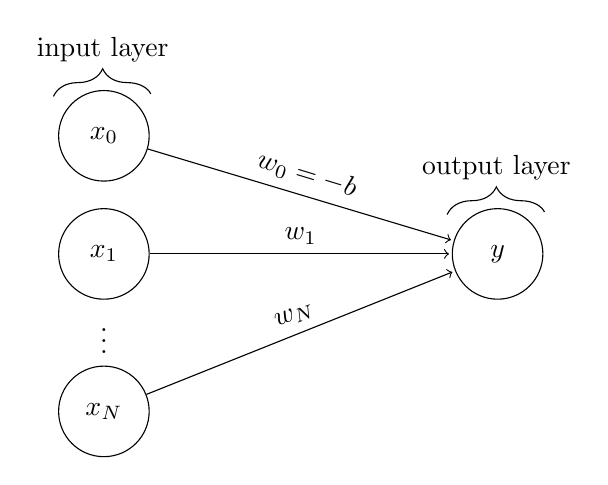
\begin{tikzpicture}[shorten >=1pt]
  	\tikzstyle{unit}=[draw,shape=circle,minimum size=1.15cm]
  	
  	\node[unit](x0) at (0,3.5){$x_0$};
  	\node[unit](x1) at (0,2){$x_1$};
  	\node(dots) at (0,1){\vdots};
  	\node[unit](xn) at (0,0){$x_N$};
  	
  	\node[unit](y1) at (5,2){$y$};
%  	\node(dots) at (4,1.5){\vdots};
%  	\node[unit](yk) at (4,0.5){$y_K$};
  	
  	\draw[->] (x0) -- node[above, rotate = -17]{\( w_0 = -b \)} (y1);
%  	\draw[->] (x0) -- (yk);
  	
  	\draw[->] (x1) -- node[above]{\( w_1 \)}(y1);
%  	\draw[->] (x1) -- (yk);
  	
  	\draw[->] (xn) -- node[above, rotate = 20]{\( w_N \)}(y1);
%  	\draw[->] (xn) -- (yk);
  	
  	\draw [decorate,decoration={brace,amplitude=10pt},xshift=-4pt,yshift=0pt] (-0.5,4) -- (0.75,4) node [black,midway,yshift=+0.6cm]{input layer};
  	\draw [decorate,decoration={brace,amplitude=10pt},xshift=-4pt,yshift=0pt] (4.5,2.5) -- (5.75,2.5) node [black,midway,yshift=+0.6cm]{output layer};
  	\end{tikzpicture}
  	\caption[Network graph of a perceptron with $N$ input units.]{The perceptron consists of $N$ input units and at least one output unit. All units are labeled according to their output: $y = H(z)$ in the case of the output unit; $x_n$ in the case of input units. The input values $x_n$ are propagated to the output unit using a weighted sum, in other words \( z = \bm w^{\intercal}\bm x \). An additional input value $x_0 := 1$ is used to include the biases as weights.}
  	\label{fig:perceptron}
\end{figure}

To describe this more precisely, let $\bm{X}=\{\bm x_n\}_{n=1}^{N}$ be the data, and \( \bm{T} =\{t_n\}_{n=1}^{N},\; t_n\in \{0,1\} \;\forall n \) be the labels. We will refer to the points \( \{(x^n,t^n)\}\subset\bm{X}\times \bm{T} \) as the training set. Then the perceptron algorithm seeks to determine the class of a new data point \( \bm x \) by using a function of the form
\begin{equation}\label{perceptron}
y = H(\bm w^{\intercal} \bm x).
\end{equation}
Here \( \bm w \) is a vector of real weights determined through training and  \( H(v) \) is the Heaviside step function
\[ H(v) =\begin{cases}
 			1 &\text{ if }v\geq 0\\
 			0 &\text{ if }v<0
		 \end{cases} 
\]

In practice, a bias term \( b \) is added to equation \ref{perceptron}, so that it becomes \( y = H(\bm w^{\intercal} \bm x +b) \). This is most usually done by adding an extra feature to all of our data points while training. This extra feature is always set to 1.  An additional weight is also appended to the weight vector \( \bm w \) so that the model still looks like \ref{perceptron}. The effect of bias is to change where the perceptron activates, and makes it harder to `fire' (\textit{i.e.} give a positive output for a given input). This also has the effect of allowing the model to center the data, as would happen with a bias in the regression setting.

%talk a bout finding weight vis gradient descent, this is easier w/ smooth activation lead into logit
The act of training for a perceptron is choosing weights \( \bm w \) so that \( H(\bm w^{\intercal} \bm x_n) = t_n\;\forall (x_n,t_n)\in \mathcal{X}\times \mathcal{T} \). The hope is that this will generalize well to data points not seen in the training set.  The point emphasized in the Minsky book \cite{Minsky90Perceptron} is that training will only work if the two classes in the training set are linearly separable.  This only applies to single layer perceptrons, as one can create a NAND gate from a single layer perceptron, so using multiple perceptrons one could conceivably approximate any function to arbitrary precision.

%single layr as logit regression
%\subsection{Single Layer Network as Logistic Regression}
The perceptron algorithm also includes methods for training, but these are not in common use today.  More modern architecture use the backpropagation algorithm, which requires gradient descent.  The problem with perceptrons in that context is that the derivative of the Heaviside step function is zero. 

The use of the Heaviside function in the perceptron is called an activation function.  In more modern neural networks, activation functions with non-zero derivative allow use of backpropagation and gradient descent.  The discussion in section \ref{logisticReg} mentions the sigmoidal activation function.  As discussed there, if we replace the Heaviside step function with the sigmoid function, then we are actually performing logistic regression.  We will refer to perceptrons using the sigmoidal activation function as sigmoidal neurons.

%multi-layer multiclass network
\subsection{Multilayer Perceptron as a Multi-Class Classifier}
The multilayer perceptron (MLP) is actually built out of several sigmoidal neurons.  The MLP we describe has a single hidden layer, which means that the output of one sigmoidal neuron becomes the input for the next neuron.  Figure \ref{fig:MLP} below gives an example of a single hidden layer MLP.

\begin{figure}[ht]
	\centering
	\begin{tikzpicture}[shorten >=1pt,->,draw=black!50, node distance=\layersep]
	\tikzstyle{every pin edge}=[<-,shorten <=1pt]
	\tikzstyle{neuron}=[circle,fill=black!25,minimum size=17pt,inner sep=0pt]
	\tikzstyle{input neuron}=[neuron, fill=green!20];
	\tikzstyle{output neuron}=[neuron, fill=red!20];
	\tikzstyle{hidden neuron}=[neuron, fill=blue!20];
	\tikzstyle{annot} = [text width=4em, text centered]
	
	% Draw the input layer nodes
	\foreach \name / \y in {1,...,5}
	% This is the same as writing \foreach \name / \y in {1/1,2/2,3/3,4/4}
	\node[input neuron] (I-\name) at (0,-\y) {\(x_\y\)};
	
	% Draw the hidden layer nodes
	\foreach \name / \y in {1,...,6}
	\path[yshift=0.5cm]
	node[hidden neuron] (H-\name) at (\layersep,-\y cm) {\(z_\y\)};
	
	% Draw the output layer nodes
	\foreach \name / \y in {1,...,3}
		\node[output neuron,pin={[pin edge={->}]right:\(\hat{y}_\y\)}] (O-\name) at (2*\layersep,-1 cm-\y cm) {\(y_\y\)};
	
	% Connect every node in the input layer with every node in the
	% hidden layer.
	\foreach \source in {1,...,5}
	\foreach \dest in {1,...,6}
	\path (I-\source) edge (H-\dest);
	
	% Connect every node in the hidden layer with the output layer
	\foreach \source in {1,...,6}
	\foreach \dest in {1,...,3}
	\path (H-\source) edge (O-\dest);
	
	% Annotate the layers
	\node[annot,above of=H-1, node distance=1cm] (hl) {Hidden layer};
	\node[annot,left of=hl] {Input layer};
	\node[annot,right of=hl] {Output layer};
		
	\end{tikzpicture}
		\caption[Network graph of a multilayer perceptron.]{A graph model of a single hidden layer MLP with 5 inputs, 3 output and 6 hidden layer nodes. The output of each layer is determined by composing a linear map with a nonlinear map. The general form of this nonlinear map is determined at the outset, though it may have trained parameters. The linear map is determined through a set of learned weights.}
	\label{fig:MLP}
\end{figure}

Neural networks such as the MLP are often called feedforward neural networks.  This is because at each stage of computation information is only passed forward toward the output nodes.  The general pattern of feedforward nets is that each node passes a weighted sum of previous nodes through an activation function.  We have already mentioned two activation functions, Heaviside and sigmoidal. Other common activation functions are hyperbolic tangent, rectified linear unit (RELU), and sigmoid linear unit \cite{elfwingSiLU}.

In the case of the MLP, each of the hidden layer nodes work as a sigmoidal neuron \textit{i.e.} \( z_l = \gs(\bm w_{1l}^{\intercal}\bm x) \). Likewise, each of the output layers can be expressed as a sigmoidal neuron, \( y_k = \gs(\bm w_{2k}^{\intercal}\bm z) \). This view is not consistent with a desire to express the output in terms of a probability. This is particularly important if we wish to use the MLP as a multi-class classifier, as we wish to interpret the outputs as \( P(k_n=k|\bm x_n) \).

While each individual output is a log odds in the sense of logistic regression, together we cannot interpret each individual \( y_k \)  as a probability.  In particular, we have no guarantee that \( \sum_k y_k=1 \).  To fix this, we may pass the outputs \( y_k \) through the softmax function \textit{i.e.} 
\begin{equation}\label{MLPsoftmax}
\hat{y}_k = \frac{e^{y_k}}{\sum_{j=1}^{K} e^{y_j}}
\end{equation}

Passing the output through a softmax function has the effect of guaranteeing that \( \sum_k y_k=1 \), but if we are to interpret \( \hat{y}_k \) as a probability, then it must be regarded as a Gibbs distribution.  From a mathematical standpoint this changes the interpretation of \( y_k \) to an approximation of an energy function.  To be consistent with this interpretation, we must be careful in our choice of cost function.  This becomes more apparent when we consider the role of backpropagation in training.

\subsection{Backpropagation}\label{subsect:backprop}
Backpropagation (BP) was modernly popularized as a method for training neural networks by Rumelhart et. al. \cite{rumelhart1986learning} in 1986. Similar training methods had been used earlier, \textit{e.g.} Linnainmaa \cite{Linnainmaa1976}, in the context of optimization. Backpropagation for use in neural network training was first used by Paul Werbos in his 1974 thesis \cite{werbos1994roots}. Brief histories of the development of BP can be found in Griewank \textit{et.al.} \cite{griewank2008deriv}, Schmidhuber \cite{Schmidhuber_2015}, and Goodfellow \textit{et.al.},\cite[see ch6.6]{Goodfellow-et-al-2016}. The practical development and popularization of BP led to a very active period of research in multilayer neural networks.

While BP is often described as `just gradient descent', it is the case that BP actually refers to a specific method for calculating the gradient of the loss function with respect to the weights.  Backpropagation relies heavily on the chain rule, and the architecture of perceptron inspired neural networks. We will use a simple neural network model to help describe BP.  We draw most of the inspiration for this example from the book by Goodfellow  et. al. \cite[ch6.5]{Goodfellow-et-al-2016}

The goal of BP is to adjust the weights by subtracting off the gradient of the cost function with respect to the weights.  The key realization of BP is that with the correct network setup, this may be done by passing information backwards through the graph.  

Recall that the typical role of a layer in a feedforward neural net is to pass forward predictions based on information from the previous layer.  The role of layer \( \ell \) during training with backpropagation is to pass forward the predictions as usual. Then during the backward pass layer \( \ell \) updates its own weights \( W_{\ell} \) using gradient descent and the chain rule. Finally the layer passes back the new gradient of the loss with respect to the output \( \bm z_{\ell-1} \)of the previous layer.  Figure \ref{fig:backprop} gives a high level model of this process.

\begin{figure}[ht]
	\centering

%\usetikzlibrary{arrows}
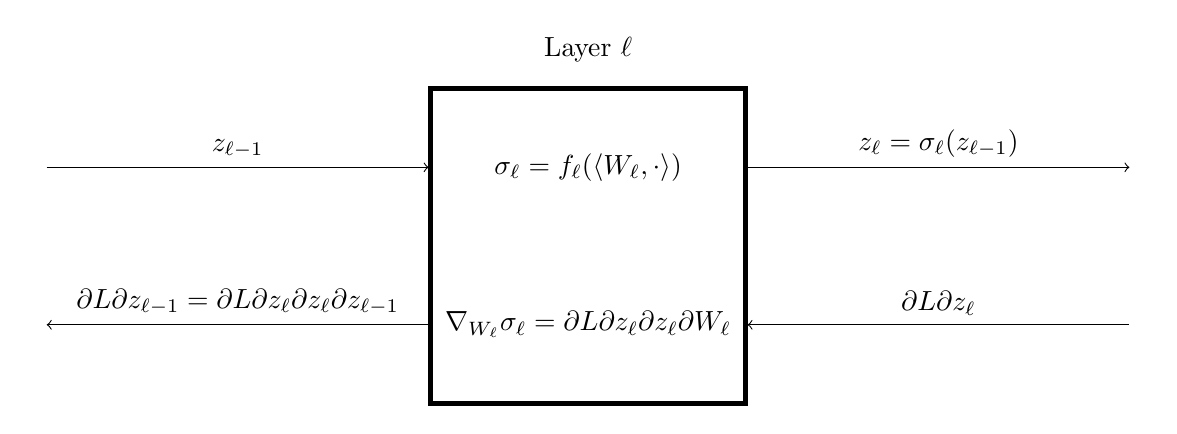
\begin{tikzpicture}

\draw [ultra thick] (-2.5,2.5) rectangle (1.5,-1.5);
\node (v1) at (-7.5,1.5) {};
\node (v2) at (-2.4,1.5) {};
\node (v4) at (-2.4,-0.5) {};
\node (v3) at (-7.5,-0.5) {};
\node (v5) at (1.4,1.5) {};
\node (v6) at (6.5,1.5) {};
\node (v8) at (6.5,-0.5) {};
\node (v7) at (1.4,-0.5) {};
\draw  [->](v1) edge node[above]{\(\bm z_{\ell-1}\)}(v2);
\draw  [<-](v3) edge node[above]{\(\dfrac{\partial L}{\partial \bm z_{\ell-1}}=\dfrac{\partial L}{\partial \bm z_{\ell}}\dfrac{\partial \bm z_{\ell}}{\partial \bm z_{\ell-1}}\)}(v4);
\draw  [->](v5) edge node[above]{\(\bm z_{\ell} = \bm \sigma_{\ell}(\bm z_{\ell-1})\)}(v6);
\draw  [<-](v7) edge node[above]{\(\dfrac{\partial L}{\partial \bm z_{\ell}}\)}(v8);
\node at (-0.5,1.5) {\(\sigma_{\ell} = \bm f_{\ell}(\langle \bm W_{\ell}, \cdot \rangle)\)};
\node at (-0.5,-0.5) {\(\nabla_{\bm W_{\ell}}\sigma_{\ell} = \dfrac{\partial L}{\partial \bm z_{\ell}}\dfrac{\partial \bm z_{\ell}}{\partial \bm W_{\ell}}\)};
\node at (-0.5,3) {Layer $\ell$};
\end{tikzpicture}
	\caption[Conceptualized model of a single network layer.]{A model of a single layer in a neural network. For the feedforward pass it calculates  \(\bm z_{\ell} = \bm \sigma_{\ell}(\bm z_{\ell-1}) = \bm f_{\ell}(\langle \bm W_{\ell},\bm z_{\ell-1}\rangle) \).  On the backward pass it calculates \( \dfrac{\partial L}{\partial \bm W_{\ell}} \) and \( \dfrac{\partial L}{\partial \bm z_{\ell-1}} \). The layer uses \( \dfrac{\partial L}{\partial \bm W_{\ell}} \) to update its own weights with gradient descent. The layer passes \( \dfrac{\partial L}{\partial \bm z_{\ell-1}} \) to the previous layer to use.}
	
\label{fig:backprop}
\end{figure}

While the diagram in figure \ref{fig:backprop} implies that the backpropagation algorithm only uses chain rule, in reality it may be a bit more complicated.  Since \( \gs_{\ell}:\R^{d_{\ell-1}}\rightarrow \R^{d_{\ell}}\) is a non linear multivariate function, taking derivatives can be complicated.  Further, the parameters \( \bm W_{\ell} \) might be part of a higher dimensional linear map (e.g matrix, tensor). For such situations we need to be more careful in calculating gradients.  While many references address this problem, \cite{matGradChain} offers a good treatment of the chain rule in such situations. Section \ref{subsect:derivNotation} covers this in more detail.

Finally it is worth noting that in many situations, backpropagation can be simply calculated in a coordinate manner.  This is because much of the structure of neural nets gives an implied coordinate system to each layer.  It is also a good reason that one must be careful in the choice of cost function. When an appropriate cost function is chosen, backpropagation becomes a quick operation. This helps explain why backpropagation is so popular in recent neural net training.
		\subsection{Derivative Notation}\label{subsect:derivNotation}

Before backpropagation resurfaces in chapter \ref{respLayer}, this section establishes important notation standards.  In the literature \cite{abraham1967transversal, manton2012differential, magnus1985matrix, matGradChain} there are several different notations used for differentiation of functions \( f:\R^n\rightarrow \R^m \). Each author seems to prefer their own notation, and while these notations often overlap, reading various papers quickly becomes confusing without precise communication. This section seeks to establish a reference for derivative notation to be used through the remainder of chapter \ref{respLayer}.

In \citep{patternnet}, care is taken to distinguish the Frech\'et (or contravariant) derivative of a function from the gradient (or covariant derivative) of the same function. Given a vector valued function \( f:\R^n\rightarrow\R^m \), the Frech\'et derivative of \( f \) at \(x\) is the linear map \( A_{ f(x)}:\R^n\rightarrow\R^m \) defined by
\begin{equation}\label{eqn:frechetDefn}
	\lim_{\norm{\bm h}\rightarrow 0} \frac{\norm{f(\bm x+\bm h)-f(\bm x)-A_{f(x)}(\bm h)}}{\norm{\bm h}}=0.
\end{equation}
Provided such a map exists, it is unique.  In particular if \( n,m<\oo \), and \( \pdv{f}{\bm x} = \left(\pdv{f_i}{x_j}\right)_i^j \) is the matrix of partial derivatives (or Jacobian matrix) of \( f \), then \( A_{f(x_0)}(h) = \eval{\pdv{f}{\bm x}}{x_0}\cdot h \).  It is worth noting that the existence of a continuous Jacobian matrix for \( f \) guarantees \( f \) has a Frech\'et derivative.  The reverse implication is not true, \( f \) can have a Frech\'et derivative but not have continuous partials everywhere.

The Frech\'et derivative of \( f \) at the point \( \bm x\in \R^n \) is often denoted by \( Df(\bm x) \), a convention which this dissertation will follow.  The notation \( Df(\bm x)[\bm h] \) works when necessary to discuss both the point \( \bm x \) at which the derivative is being taken, and the direction \( \bm h \) on which it is acting. In this sense it may be said that \( Df \) is a map \( Df:\R^n\rightarrow L(\R^n,\R^m)\). Here, \( L(V,W) \) is the collection of all linear maps from one real vector space \( V \) to another real vector space \( W \).  

Given this notation for the Frech\'et derivative, denote by \( \nabla f(\bm x) \) the gradient of \( f \). A function \( f:\R^n\rightarrow \R^m \) only has a gradient if \( m = 1 \). In this case the gradient is a map \( \nabla f:\R^n\rightarrow\R^n \)such that for all \( \bm x, \bm h \in \R^n \)
\begin{equation}\label{eqn:gradDef}
 Df(\bm x)[\bm h] = \<\bm h, \nabla f(\bm x)\>.
\end{equation} 
Here the angle brackets denote the standard euclidean inner product on \( \R^n \).  Because the gradient of a scalar valued function is a vector valued map, it is possible for \( \nabla f \) to be differentiable. In this case the resulting derivative is called the \textit{Hessian} of \( f \) and will be denoted by \( \nabla^2 f. \) 

An analog of the gradient for functions \( f:\R^n\rightarrow\R^m \) with \( m\geq 1 \) is the adjoint operator of \( Df \). The adjoint operator of any linear map \( A\in L(\R^n,\R^m) \) is the map \( A^{\ast}\in L(\R^m,\R^n) \) such that \( \forall\; x\in\R^n,\) \(y\in\R^m, \) 
\[ \<A(x),y\>_{\R^m} = \<x,A^{\ast}(y)\>_{\R^n}. \]
Since \( Df:\R^n\rightarrow L(\R^n,\R^m) \), the definition of an adjoint operator \( D^{\ast}f:\R^n\rightarrow L(\R^m,R^n)\) depends on the point \( x\in\R^n \) at which it is evaluated.  Thus \( D^{\ast}f \) is defined by 
\begin{equation*}
\<Df(x)[h],u\>_{\R^m} = \<h,D^{\ast}f(x)[u]\>_{\R^n}
\end{equation*}
holding \( \forall\; x,h\in\R^n,\) \(y\in\R^m.\) Aside from the reliance of the definition on the inner product, the adjoint derivative 

When dealing with linear maps between \( \R^n \) and \( \R^m \), all the maps can be recognized as matrix maps; in this case the adjoint is the transpose of the matrix, \textit{i.e.} \( A^\ast = A^{\intercal} \). This is not true for general vector spaces \( V,W \) over \( \R \) as there may be linear maps which cannot be recognized as matrices. An important example is when \( V,W \) are matrix algebras over \( \R \).

Thus it will not be assumed \textit{a priori} that the derivative maps \( Df,\;D^{\ast}f \) are matrix maps.  In fact, for some of the functions used in chapter \ref{respLayer}, \( Df,\;D^{\ast}f \) will not just be linear maps, but multilinear maps, or tensors.  In this case there are still analogs of adjoint operators but more care must be taken in describing them. Discussion of such details will come when necessary.

Since backpropagation does gradient descent, it must calculate the gradient of the loss $L$ with respect to weights $W$. In figure \ref{fig:backprop}, this is shown to be done via the chain rule, but in the general case more care must be applied. The following lemma makes this much easier.
\begin{lemm}\label{gradChain}
	Let $U,V$ be real Riemannian Manifolds and $f:V\rightarrow \R$ and $g:U\rightarrow V$ be smooth maps.  Then if $h=f\circ g$, we have that 
	\[\nabla h=D^{\ast}g[\nabla f\circ g]\]
	where $\nabla h,\nabla f$ are the gradients of $h$ and $f$ respectively, and $D^{\ast}g$ represents the adjoint linear operator of $Dg$ with respect to the metrics on $TV$ and $TU$.
\end{lemm}
\begin{proof}
	This is lemma 4.1 of Theis \citep{matGradChain}. This proof adapts it for use in this dissertation. 
	
	First, let $u \in U$ and $x\in T_uU$ be arbitrary. Because $f,g$ are smooth, they induce maps $Dg(u):T_uU\rightarrow T_{g(u)}V$ and $Df(g(u)):T_{g(u)}V\rightarrow \R$.
	It is given (by definition) that $Dh(u)[x]=\langle \nabla h(u),x\rangle_{T_uU}$. Further, it is clear that $Dh(u):T_uU\rightarrow\R$ is given by $Dh(u)[x]=D(f\circ g)(u)[x]=Df(g(u))[Dg(u)[x]]$. 
	
	Now $Df(g(u))[Dg(u)[x]]=\langle\nabla f(g(u)),Dg(u)[x]\rangle_{T_{g(u)}V}$.  Then for the linear operator $Dg(u):T_uU\rightarrow T_{g(u)}V$, the adjoint linear operator $D^{\ast}g$ is defined by the equation $\langle y,Dg(u)[x]\rangle_{T_{g(u)}V}=\langle D^{\ast}g(u)[y],x\rangle_{T_uU}$ for $x\in T_uU$ and $y\in T_{g(u)}U$.  This gives  
	\[Df(g(u))[Dg(u)[x]]=\langle\nabla f(g(u)),Dg(u)[x]\rangle_{T_{g(u)}V}=\langle D^{\ast}g(u)[\nabla f(g(u))],x\rangle_{T_uU}.\]
	So that $\langle \nabla h(u),x\rangle_{T_uU}=\langle D^{\ast}g(u)[\nabla f(g(u))],x\rangle_{T_uU}$, and as $u,x$ were arbitrary, the theorem is proved.
\end{proof}

A key aspect of the proof above is the use of the metric on $U$ and $V$. This allows identification of tangent spaces to their duals, $TU\cong TU^{*}$ and  $TV\cong TV^{*}$, to define $Dg^{*}$ appropriately. this is not surprising as the definition for the gradient of \( f \) in equation \ref{eqn:gradDef} is closely tied to the inner product on the domain of \( f \).  It follows that wherever derivatives will be used in this dissertation, the appropriate choice of metric (and thus inner product) on the tangent space will be essential. 

%  It may be worth mentioning information geometry and natural gradient descent here. \textcolor{red}{(Fix Later)}. NOPE! 5/11/2020 this is something for a future paper.
Because all the spaces involved can be embedded in \( \R^n \) for some \( n \), many calculations in chapters \ref{Algorithm} and \ref{respLayer} use the inner product on $\bm M=L(\R^N,\R^K)$, defined by the Frobenius inner product $\langle A,B\rangle=\op{tr}(A^{\intercal}\cdot B)$. The map $\op{vec}:\bm M\rightarrow \R^{KN}$ given by stacking the columns of $M$ is a diffeomorphism, and the Frobenius inner product on $\bm M$ is equivalent to the standard euclidean inner product on $\R^{KN}$.  In short, the following diagram commutes.

\begin{equation}\label{eqn:vecfrobcommute}
\begin{tikzcd}
\bm M\times \bm M \arrow[dr, "\op{Frob}" left] \arrow[r, "\op{vec}" above] & \R^{KN}\times \R^{KN} \arrow[d, "\op{euc}" right]\\
[1em] & \R
\end{tikzcd}
\end{equation}
Here $\op{Frob}$ and $\op{euc}$ represent the inner product (metric) on each of the spaces.  

Finally, it is worth mentioning that when necessary, such as in the proof of lemma \ref{gradChain}, discussions reference the tangent space \( TU \) of a Riemannian manifold \( U \).  Since all the spaces here are generally euclidean, such notational references help distinguish the space \( U \) from \( T_uU \), vectors tangent to some point \( u\in U \). The full strength of considering these spaces as manifolds will not be used.
%\Ryan{Talk about what each of these are and their relation to the set of partials.  Mention that for maps from Rm to Rn these are pretty straightforward for the first derivative.  For higher order derivatives it gets messy (tensors). This is also true for maps from matrix spaces to matrix space, but the vec map can turn it into the other situation.  Ultimate goal of chapter: find a vectorized algorithm for computing \( \pdv{L}{F} = \pdv{L}{Y}\pdv{Y}{F} \). If these are both tensors, order matters!}
	\section{Responsible Clustering Algorithms}
		%!TEX root = ../Dissertation_RC.tex

\subsection{$K$-means algorithm}\label{kmeans}
The $K$-means algorithm has been in use for several decades.  Though the first 
mention of the algorithm by name was given by MacQueen in 1967 \cite{
macqueen1967kmeans} the idea had been around for some time.  The standard  
algorithm was used at Bell Labs in 1957 \cite{Lloyd82} for pulse code 
modulation.  Pollard \cite{pollard1981,pollard1982} showed that the $K$-means 
algorithm is consistent in a very precise sense.  Today the algorithm is used 
in many applications \cite{AutoClass1,AutoClass2}, and can be found in many 
good books on machine learning.
\cite{Bishop1995,MacKay2002,BishopBook,hastie09esl,MML_2019}

The outline below is primarily compiled from chapters 20 and 22 of MacKay
\cite{MacKay2002}, though the Bishop and Deisenroth books 
\cite{BishopBook,MML_2019} played a big role.  

The \(K\)-means algorithm is used for vector quantization and for data 
clustering.  It is so named because it separates data points into $K$ distinct 
groups, each characterized by a `mean' \(\bm m_k,\, k= 1,\ldots,K\).  In the 
case that the \(K\)-means algorithm is being used for clustering, these means 
are the cluster centers and each data point is assigned to the closest mean.
In this situation it is the case that 
\[\bm m_k = \frac{\sum_{n=1}^{N} r_k^n \bm x^{(n)}}{N_k}\]
where 
\begin{equation*}
r^n_k = \begin{cases}
			1 & \text{if } \bm x^{(n)} \text{ is closest to } \bm m_k\\
			0 & \text{otherwise}
		\end{cases}
\end{equation*}
and \(N_k = \sum_{n=1}^{N} r^n_k\).  In other words, the means \(\bm m_k\) are 
literally the means of the assignment clusters.

Of course we cannot understand `closest' without first defining a distance 
function  on the underlying data space.  For the original \(K\)-means 
algorithm, the distance was the manhattan distance, though we will use a 
scaled square of the euclidean distance:
\[d(\bm x, \bm y) = \frac 12 \sum_i (x_i-y_i)^2.\]
It is worth noting that the choice of distance in this sense is somewhat 
arbitrary. In most descriptions of the algorithm, euclidean distance is used 
to aid visualization.

To implement the \(K\)-means algorithm, start with \(K\) distinct means.  
A common practice is to use randomly sampled data points 
\(\{\bm m_1 = \bm x^{(n_1)},\ldots,\bm m_K = \bm x^{(n_K)}\}\). Then iteratively 
do the following:
\begin{enumerate}
	\item For each data point, \(\bm x^{(n)}\), set 
	\(\hat{k}_n = \argmin_k d(\bm x^{(n)},\bm m_k)\).
	\item Set \(r_{\hat{k}_n}^{n} = 1\), for each \(n\). Set all other 
	\(r_k^n = 0\)
	\item Calculate \(N_k = \sum_{n=1}^{N} r^n_k\) and 
	\[\bm m_k^{new} = \frac{\sum_{n=1}^{N} r_k^n \bm x^{(n)}}{N_k}.\]
	If \(N_k = 0\), \(\bm m_k^{new} = \bm m_k\).
	\item If \(d(\bm m_k ,\bm m_k^{new})\) is within a predefined tolerance, 
	stop.  Otherwise set \(\bm m_k = \bm m_k^{new}\) and repeat at step 1.
\end{enumerate}
%algorithm? soft k means? generalized k means?
In the literature, it is common to see steps one and two listed as the 
assignment step, and steps three and four as the update step.  

The easiest way to see that this algorithm terminates is to recognize that the 
function \[L := \sum_{n=1}^{N} d(\bm x^{(n)},\bm m_{\hat{k}_n})\]
either stays the same or decreases at each update step.  In this sense, \(L\) 
acts as a Lyapunov function for the \(K\)-means algorithm.

One problem with k-means clustering that is particularly relevant to this 
paper comes when the clusters do not have equal representation in the data.
as an example:\textcolor{red}{(input example)}

In this case, the cluster means are often slightly off center and some data 
points are be inappropriately labeled. %voronoi diagrams? 
One way to fix this is with \textit{soft responsibility}. 
\[r_k^{(n)} = \frac{\exp(-\gb d(\bm x^{(n)},\bm m_k))}
{\sum_i \exp(-\gb d(\bm x^{(n)},\bm m_i))}\]

The idea behind soft responsibility is that each cluster center is partially 
responsible for each data point.  The amount of responsibility \(r_k^{(n)}\) 
of \(\bm m_k\) for the data point \(\bm x^{(n)}\) ought to be inversly 
proportional to \(d(\bm x^{(n)},\bm m_k)\). That is, cluster centers closer to 
data points have greater responsibility for those data points.  

The factor \(\gb\) included here is an inverse temperature, or stiffness 
algorithm, and it can be set at the beginning or iteratively.  In futher 
refinements of the soft $K$-means algorithm, each cluster center has its own
\(\gb_k\), and at each iteration \(\gb_k = \dfrac{1}{\gs_k^2}\) where 
\(\gs_k^{2}\) is the weighted sample variance of the data points assigned to 
cluster $k$.
\[\gs_k^{2} = \frac{\sum_n r_k^{(n)}d(\bm x^{(n)},\bm m_k)}{N_k}\]

Further refinements to this algorithm can be found in MacKay's book, and were 
also developed in the software AutoClass. \cite{MacKay2002,AutoClass1,AutoClass2}

		%!TEX root = ../Dissertation_RC.tex

\subsection{Expectation Maximization} \label{emAlg}
Upon close inspection, it can be seen that the soft \(K\) means algorithm is 
very similar to the Expectation Maximization (or EM) algorithm for Gaussian 
Mixture Models.  What follows is a brief overview of expectation maximization
and the relation of this algorithm to responsibility as discussed in section 
\ref{kmeans}. The discussion below roughly follows discussions available in 
Bishop and other sources \cite{MML_2019, BishopBook, hastie09esl}.

EM was first described in a paper by Dempster et. al. \cite{Dempster77EM}.
The basic idea behind EM is to add hidden or latent variables to a modeling
problem in such a way that maximum likelihood estimation is made easier.  The 
heuristic of this approach is that the latent variables are simply unobserved 
features of the data.  

To be more precise, suppose we are given data $ x $ and we want to fit a model 
with parameters $ \gt $ for the pdf \( p(x|\gt) \) using maximum likelihood 
estimation. In many cases this is an intractable problem that can be simplified
by considering the conditional pdf
\begin{equation}\label{emcond}	
p(x|\gt,z).
\end{equation}

Now as \( z \) are latent variables, we must place a prior \( p(z) \) on the 
distribution of \( z. \) Using \ref{emcond}, and the law of total probability 
we may write
\begin{equation}\label{emtotprob}
p(x|\gt)=\int_{\mathcal{Z}} p(x|\gt,z)p(z)\;dz.
\end{equation}
Where the integral is taken over the space of possible latent variables.

In practice, the integral in \ref{emtotprob} can easily diverge.  The trick is
to choose \( z \) and \( p(z) \) in a manner that avoids this difficulty. 
The EM algorithm is an iterative

%One simplification used for clustering is the assumption that \( z \) is discrete.
%Even if \( z \) is not discrete, we may use Bayes rule to update the prior 
%\(p(z)\).

	\section{Clustering with Mixture Models}
		\section{Mixtures in general}\label{sec1}
 While humans can quickly pick out patterns for data that can be easily visualized, the problems of evaluating high dimensional data, teaching computers to do what humans do easily (e.g.: character recognition), or even of finding new and unknown patterns are interesting from a mathematical perspective.  We will discuss some of the known clustering algorithms available and include some examples of interest.  Examples of interest may include data sets where a given algorithm does especially well, and will include ones where the algorithms work very poorly.
 
In some sense, Clustering may be considered an example of distribution inference given data.  If we have several samples, and a good idea that each sample comes form a different distribution, we can ask two different, but related questions.  First, what are the distributions that were sampled from?  Second, how can we infer which data points came from which distribution? In general, the first question may be called clustering, and the second question classification. For now we will focus mostly on clustering and return to classification later.

To make the question more precise, consider the problem of sampling from $K<\oo$ probability distributions with pdfs \(f_k(x,\gt),\; 1\leq k\leq K\). Each distribution $f_k(x,\gt)$ is chosen at random with proportion $\pi_k^\ast$, $\sum_k \pi_k^\ast=1$.  This is a situation that is mimicked easily enough in Monte Carlo simulations, and is common in applications.  As a two stage experiment, we work as follows to select a point in $x_n\in\R^I$:
\begin{enumerate}
\item Stage 1: From the $K$ possible distributions, select a label $k_n$ with probability $P(k_n=k)=\pi_{k}^\ast$.
\item Stage 2: Sample $x_n$ from $f_{k_n}(x)$
\end{enumerate}

Given $N$ such data points, $D=\{x_n\}_{n=1}^{N}$, clustering then is the problem of estimating the parameters $\gt=\{\bm\pi^\ast,\ldots\}$, where $\bm\pi^\ast\defined\{\pi_k^\ast\}_{k=1}^{K}$. This essentially assigns each of the data points $\bm x_n$ as a sample from a particular pdf in \(f_k(x,\gt),\; 1\leq k\leq K\).  We have in this case 
\[P(x_n|\gt)=\sum_k P(x_n|k_n=k,\gt) P(k_n=k, \gt)=\sum_k \pi_k^\ast f_k(x_n,\gt).\]

One reason that we choose to estimate the parameters $\{\pi_k^\ast\}$ first is that often our other estimates for the remaining parameters $\gt$ are not independent of our choices for the labels.  We proceed as inspired by \textit{Information Theory, Inference, and Learning Algorithms}\citep{MacKay2002}.

Using Bayes' rule, we may formulate a strategy for recovering the parameters $\{p_k\}_{k=1}^{K}$. Given the data $D$, we ask what is the likelihood that the labels chosen were $\{k_n\}_{n=1}^{N}$, given some prior distribution of the labels as $\{\pi_k\}_{k=1}^{K}$. That is to say that $P(k_n=k, \gt)=\pi_k$, for example the naive assumption would be $\pi_k=\frac 1K$.

Bayes rule gives:
\begin{align}\label{Bayes1}
P(k_n=k|\{x_n\},\{\pi_k\})&=\frac{P(x_n|k_n=k)P(k_n=k)}{\sum_{k'}P(x_n|k_n=k')P(k_n=k')} \nonumber \\
						  &=\frac{\pi_k f_k(x_n)}{\sum_{k'}\pi_{k'} f_{k'}(x_n)}
\end{align}

%For a more visual example, consider the ``stacked" functions $f_k$:
%\begin{center}
%%TODO fix the grapics here, probably through a relevant MATLAB example.
%%\includegraphics[scale=.2]{piecewise4.png} 
%	\begin{tikzpicture}[scale=1.75]
%		\draw[->] (-1,0) -- (5,0) node[right] {$x_n$};
%		\draw[->] (0,-.5) -- (0,2.5) node[right] {$P(x_n|\gt)$};
%		\draw[thick,red] plot[samples=100, smooth, domain=-1:5,id=exp1] (\x,{5*exp(-(\x-1)^2/1)/(2*1*sqrt(2*3.14159))});
%		\draw[thick,blue] plot[samples=100, smooth, domain=-1:5,id=exp2] (\x,{5*(exp(-(\x-1)^2/1)/(2*1*sqrt(2*3.14159))+exp(-(\x-2)^2/4)/(4*2*sqrt(2*3.14159)))});
%		\draw[thick,green] plot[samples=100, smooth, domain=-1:5,id=exp3] (\x,{5*(exp(-(\x-1)^2/1)/(2*1*sqrt(2*3.14159))+exp(-(\x-2)^2/4)/(4*2*sqrt(2*3.14159))+exp(-(\x-3)^2/9)/(3*sqrt(2*3.14159)))});
%		\draw[thick] plot[samples=100, smooth, domain=-1:5,id=exp4] (\x,{5*(exp(-(\x-1)^2/1)/(2*1*sqrt(2*3.14159))+exp(-(\x-2)^2/4)/(4*2*sqrt(2*3.14159))+exp(-(\x-3)^2/9)/(3*sqrt(2*3.14159))+exp(-4*(\x-2.5)^2)/(2*1*sqrt(2*3.14159)))});
%		\foreach \x in {-1}
%			\draw[xshift=\x cm] (0pt,2pt) -- (0pt,-2pt) node[below]{$\x$};
%		\foreach \x in {1,...,5}
%			\draw[xshift=\x cm] (0pt,2pt) -- (0pt,-2pt) node[below]{$\x$};
%			
%%		\node [below=1cm, align=flush center,text width=8cm] at (2,-.25)
%%        {
%%           % TODO create graphics here, probably through a relevant MATLAB example.
%%        };
%	\end{tikzpicture}
%\end{center}
%
%In this example, $K=4$, and priors are $\{\pi_k\}_{k=1}^{4}$.  This graphic visualizes the density 
%\[P(x_n|\gt)=\sum \pi_k f_k(x_n)\]
%where the vertical stripe is divided into regions of about $\pi_k f_k(x)$.
%Note here that we have joint distribution which is the mixed discrete-continuous distribution of $(x_n,k_n)$:
%\[P\left(x-\Delta x<x_n<x,k_n=k\right)=\pi_k\cdot\int_{x-\Delta x}^{x}f_k(x_n)\;dx.\]

We have a notion of conditional density
\begin{align*}
\frac{P\left(x-\Delta x<x_n<x,k_n=k\right)}{P\left(x-\Delta x < x_n <x+\Delta x\right)}&\approx\\ \frac{\pi_kf_k(x)\Delta x}{\sum_{k'} \pi_{k'}f_{k'}(x) \Delta x}&=P(x_n|k_n=k,\gt)
\end{align*}

The joint distribution of $\{x_n\}$ and $\{k_n\}$ is 
\[P(\{x_n\}, \{k_n\}|\{\pi_k\})=\prod_n \pi_{k_n}f_{k_n}(x_n).\]
Since we have no practical way of knowing the true labels of points $x_n$; we perform marginalization
\begin{align*}
P(\{x_n\}|\{\pi_k\})&=\sum_{(k_1,k_2,\ldots,k_N)}\prod_n \pi_{k}f_{k_n}(x_n)\\
&= \prod_n \left(\sum_{k}\pi_kf_k(x_n)\right)\\
&= \prod_n P(x_n|\{\pi_k\})
\end{align*}
where $\displaystyle{P(x_n|\{\pi_k\}) =\sum_{k}\pi_kf_k(x_n)}$

\begin{eg} Find the most likely values of $\{\pi_k\}$, given data $\{x_n\}$. We assume complete lack of knowledge, i.e. the prior distribution of $\{\pi_k\}$ is uniform on the standard probability simplex 
\begin{equation}\label{simplexDef}
	S_K:=\left\{\{\pi_k\}_{k=1}^{K}:0\leq \pi_k\leq 1; \sum_{k=1}^{K}\pi_k =1\right\}
\end{equation}

\end{eg}

\begin{soln}
Bayes says
 \[P(\{\pi_k\}|\{x_n\})=\frac{P(\{x_n\}|\{\pi_k\})P(\{\pi_k\})}{\int\int_{\ldots}\int P(\{x_n\}|\{\pi_k\})P(\{\pi_k\})\; d\pi}\]
 Remember that the prior $P(\{\pi_k\})$ is uniform.
\end{soln}
We note here that if we would perform a maximum \textit{a posteriori} estimate at this point, it would be equivalent to finding a maximum likelihood estimator for $\bm\pi^\ast$.

While the marginal probability is difficult to compute, we get a lot of mileage out of looking at the log likelihood.  We define
\begin{align*}
L&:= \ln P(\{x_n\}|\{\pi_k\}) = \sum_n \ln P(x_n|\{\pi_k\})
\end{align*}
and then maximize the likelihood on the simplex $S_K$.
We then define 
\[\{\hat{\pi}_k\}=\argmax_S L\]
The problem of finding the `correct' probability distribution $P(\{\pi_k\})$ then becomes the problem of finding the maximum likelihood estimator of $L$.  

To do this we may use the method of Lagrange multipliers. With our objective function as 
\[\mathcal{L}=L-\gl G\]
where $G(\{\pi_k\})=\sum_k \pi_k -1$, we get the system of equations:
\begin{align*}
&\pder1{\mathcal{L}}{\pi_k}=\pder1{L}{\pi_k}-\gl \pder1{G}{\pi_k}=0\qquad \; k=1,\ldots, K\\
&\pder1{\mathcal{L}}{\gl}=-G(\{\pi_k\})=0
\end{align*}
then we have 
\begin{align*}
\pder1{L}{\pi_k}&=\sum_n \pder1{}{\pi_k}\ln P(x_n|\{\pi_k\})\\
&=\sum_n \frac{f_k(x_n)}{P(x_n|\{\pi_k\})}
\end{align*}
so that the above equations becomes the system of algebraic equations
\begin{align}\label{lageq}
\sum_n\frac{f_k(x_n)}{\sum_{k'}\pi_{k'}f_{k'}(x_n)}&=\gl&k=1,2,\ldots, K\\
\sum_k\pi_k=1
\end{align}

This problem, namely of finding the posterior estimates $\{\hat{\pi}_k\}$ in this manner is well-posed.  We note that in the formation of this problem, we did not incorporate all the conditions of the simplex $S$.  Namely, some of the $\hat{\pi}_k$ could be negative. In practicality this means we need to check the boundary conditions.

%Below is a CAS generated exact solution for $N=2$ data points and $K=2$ clusters.

%TODO generate and insert an example.
	\section{A Brief Introduction to Discrete Dynamical Systems}
		%\Ryan{A \textit{short} section needs to be added here.  Mostly to cover definitions of: stable points, stable sets/manifolds, Lyapunov functions, bifurcations and any other terms unique to dynamical systems and not inference/ML. Marek suggest doing a literature `review', in the sense of citing important theorems.  Maybe a few definitions. }

This section presents some definitions from the field of dynamical systems that are relevant to the dissertation.  Many of these definitions can be found in an undergraduate text like \cite{devaney1989introduction}. The definitions in this section are mostly adapted from the review paper by Mei and Bullo \cite{mei2017lasalle}. Their paper in turn is a summarized version of the contents of a book by LaSalle \cite{lasalle1976dynsys}.

To begin, let \( \N \) represent the natural numbers, and \( \R \) the real numbers. Then \( \R^m \) is \( m \) dimensional euclidean space, and the vectors \( \mathbbm 1_m,\;\bm 0 \) denote the vectors composed entirely of 1's and 0's respectively. The notation \( \bm e_i\;1\leq i\leq m \) will denote the standard basis vectors for \( \R^m \).

For any sequence of points \( \{x_k\}_{k\in\N} \in\R^m\) use \( {x_k}\rightarrow y \) to mean that \( \norm{x_k-y}\rightarrow 0 \) as \( k\rightarrow\oo\). For a set \( S\subset\R^m \), let \( \op{Int}S \) denote the interior of \( S \). If \( S \) is a bounded set, let \( \partial S \) denote the boundary of \( S\), and \( \overbar S = \op{Int}S\cup \partial S\) be the closure of \( S \). The symbol \( \varnothing \) will denote the empty set.  

Given a map \( T:\R^m\rightarrow\R^m \), for \( n\in \N \), define \( T^n=T\circ T\circ\ldots\circ T \) to be the \( n \)-fold composition of \( T \) with itself. The study of \textit{discrete dynamical systems} is, broadly speaking, the study of such continuous maps and their compositions. 

\begin{defn}[Discrete Dynamical System]\label{defn:discDynSys}
	For \( M\subset\R^m \) the map \( \bm\tau:\ZZ\times M\rightarrow M \) describes a discrete dynamical system on \( M \) if for all \( n,k\in\ZZ \) and any \( x\in M \),
	\begin{enumerate}
		\item \(\bm\tau(0,x) = x;\)
		\item \(\bm\tau(n,\bm\tau(k,x)) = \bm\tau(n+k,x)\);\label{eqn:groupProperty}
		\item \( \bm\tau \) is continuous.
	\end{enumerate}
	If requirement \ref{eqn:groupProperty} holds for only \( n,k\geq 0 \), then \( \bm\tau \) describes a discrete \textit{semi-dynamical} system on \( M \). Thus this definition of a discrete dynamical system requires \( \bm\tau(1,x) \) to be a continuous bijection with continuous inverse (\textit{i.e.} a homeomorphism).
\end{defn}

Given a continuous map \( T:M\rightarrow M \) and some initial point \( x_0\in M \), one of the important goals of studying discrete dynamical systems is deciding whether sequences \( \{x_n\}\defined {T^n(x_0)} \) have any limit points.
\begin{defn}[Orbits]
	 Sequences of the form \( x_n = T^n(x_0) \) for some \( x_0 \in M \) are called \textit{orbits} of \(T\).(also motions or trajectories).%\Ryan{Note that motions, trajectories and orbits are actually slightly different things. A motion is a function. Trajectories and orbits are sets. it doesn't hurt to conflate the things for this paper.}
\end{defn} 
Property \ref{eqn:groupProperty} guarantees that for any \( x\in M \), there is exactly one orbit of \(T \) such that \( x_0=x \). By abuse of notation this will be called the orbit of \( x \).

\begin{defn}[Limit points]\label{defn:limitpoints}
	Given a specific point \( x\in M \) the set \( \Omega(x)\subset\R^m \) is the set of all limit points of \( x \). The point \( y\in \R^m \) is a limit point of \( x \) if there is a subsequence \( x_{n_k} \)  with \( |n_k|\rightarrow\oo \) of the orbit \( T^n(x) \) such that \( x_{n_k}\rightarrow y \).  This is the case for both dynamical and semi-dynamical systems. 
\end{defn} 
For some set \( H\subset M \), the set \( \Omega(H) \) is the set of all limit points of for \( x\in H \), \textit{i.e.} \( \Omega(H)=\bigcup_{x\in H}\Omega(x) \). 
\begin{defn}[Invariant Sets]
	The set \( H \) is called \textit{positively invariant} if \( T^n(H)\subset H\;\forall n\in\N \). A set \( H \) is called \textit{negatively invariant} if \( T^n(H)\supset H\;\forall n\in\N \). If \( T(H)=H \) then \( H \) is called \textit{invariant}.
\end{defn} 
A compact invariant set satisfies \( \Omega(H)\subset H \). For discrete semi-dynamical systems, the set \( H \) needs only to be positively invariant and compact.

Property \ref{eqn:groupProperty} is also required to guarantee uniqueness of \textit{periodic points}. \begin{defn}[Periodic points, Fixed points]
	Periodic points are those \( x\in M \) which satisfy \( T^n(x)= x \) for some \( n \).  For a periodic point \(x\), the smallest \( k\in\N \) such that \( T^k(x)=x \) is called the period of \( x \).  \textit{Fixed points} are periodic points of period 1, \textit{i.e.} \( x\in M \) such that \( T(x) = x \).
\end{defn} 
All periodic points of period \( k \) are fixed points of the map \( T^k \). If they exist, periodic points are limit points of a discrete dynamical system.

\begin{defn}[Stable set]
	For a given periodic point \( p\in M \) of period \( k \), the \textit{stable set} of \( p \) is the set of all points \( x\in M \) that eventually arrive at \( p \), \textit{i.e.} \( W^s(T,p)\defined \{x\in M| T^{k+n}(x)\rightarrow p \text{ as } n\rightarrow\oo\}. \)The stable set of a fixed periodic point is always non-empty as it contains \( p \).
\end{defn}  
\begin{defn}[Asymptotically Stable]
	A periodic point \( p \) is called \textit{asymptotically stable} if \( p\in\op{Int}W^s(T,p). \)  In other words, \( p \) is asymptotically stable if there is some \( \gd>0 \) such that \( \norm{x-p}<\gd \) implies that \( T^{k+n}(x)\rightarrow p \), where \( k \) is the period of \( p \).  
\end{defn}

\begin{defn}[Lyapunov stable]
	A point \( x\in M \) is \textit{Lyapunov stable} if points that start sufficiently near \( x \) have orbits close to \( x \). More precisely, \( x \) is Lyapunov stable if for any \( \ge>0\) there is some \(\gd>0\)  such that \( \norm{x-y}<\gd \) implies \( \norm{T^n(x)-T^n(y)}<\ge\) for all \(n\in\N \).
\end{defn}
%\Marek{I don't like the use of quantifiers as if they were verbs in sentences. This is undergraduate-like and quantifiers should be used properly, e.g. they define a variable and its range, and are before the statement that uses the variable. Alternatively, write out ``for all'' and ``there exists''. I find it easier to read, anyway.}\Ryan{agreed, thanks for the comment!}

The last definition of this section is briefly covered in the review paper \cite{mei2017lasalle}, but a more thorough treatment is given by LaSalle in chapter 1 section 6 of \cite{lasalle1976dynsys}. The definition that follows is adapted from LaSalle's work.

\begin{defn}[Lyapunov Function]
	Given a discrete (semi-)dynamical system described by iterating the continuous map \( T:M \rightarrow M\) Let \( G\subset\R^m\), \( G\cap M\neq \varnothing\) then a continuous map \( V:G\rightarrow\R \) is a \textit{Lyapunov function} for \( T \) on \( G \) if \( V(T(x))-V(x)\leq 0 \) for all \( x\in T(M)\cap G \).
\end{defn}

Generally speaking, the map \( V \) is difficult to find for a given discrete dynamical system.  However, as the following theorem shows, very powerful results come from finding a Lyapunov function.

\begin{thm}[Invariance Principle]\label{thm:invariance}\ \\%*[-.2\baselineskip]	
	If \( V \) is a Lyapunov function for \( T \)  on \( G \), define \( E\defined\{\left.x\in\overbar G\right|V(T(x))-V(x)=0\} \) and let \( H \) denote the largest invariant set in \( E \). Then if \( T^n(x)\subset G \) is a bounded orbit of \( x\in G \), there exists a number \( c\in\R \) such that \( T^n(x)\rightarrow H\cap V^{-1}(c) \).
\end{thm}

\begin{proof}
	This is theorem 6.3 of LaSalle chapter 1, section 6 \cite{lasalle1976dynsys}. The same idea is explored in a more general setting in chapter 4 of the same book, and is what allows passage to \( M\subset\R^m \). An accessible, self contained version of the proof can be found in the review paper by Mei and Bullo \cite{mei2017lasalle}.
\end{proof}
\Ryan{Write this as thm 3.1 of chapter 4 in \cite{lasalle1976dynsys}, then cite it in theorem \ref{thm:convergence}.  Maybe put this in an appendix!}
%\Ryan{Maybe a theorem about using lyapunov functions on manifolds with boundary? need lie derivative with the vector field to have constant sign. is there some small set of points where \( -\ell \) is not a lyapunov function? (nope!) Lasalle reference in lyapunov function wikipedia article may be a good book to cite. maybe also lasalle's invariance principle.}
%
%\Ryan{Kantorovich is a better argument, according to Marek. see comments in \ref{sect:expConvRate} for more.}
%		
% add a section about overfitting, generalization, and metrics for performance?
%	\biblio
%\end{document}
% \appendix
% \section{Dynamic Responsibility Code}
\begin{verbatim}
simplex_map.m
stablepoint.m
StablepointNewton.m
GMMData.m
error_samples.m
\end{verbatim}

\section{Responsible Softmax Code}
\begin{verbatim}
RespLoss.m 
FixedRespLoss.m
and dependencies
\end{verbatim}
\section{Code for Examples on GMM Data}
\begin{verbatim}
GMMoverlap.m 
Other data sets?
\end{verbatim}
\section{Code for Example on MNIST Data}
\begin{verbatim}
MNISTBenford.m
\end{verbatim}
%
% \begin{thebibliography}{99}
% And the bibliography goes here.  
% \end{thebibliography}
%
% \end{document}  
% \end{verbatim}
%
% \subsubsection{A Masters Thesis}
%
% This thesis is copyrighted, but does not have Acknowledgments or a
% Dedication.  It is written by a student in the Department of
% Mathematics. 
%
% \begin{verbatim}
% \documentclass[final]{ua-thesis}
%
% \hoffset -2.1mm
%
% \director{Advisor's Name}
% \directortitle{Professor of Mathematics}
% \degree{Master of Science}
% \degreeabbrev{M.S.}
% \department{Department of Mathematics}
% \date{1996}
%
% \title{This is a Masters Thesis}
% \author{Your Name}
% \copyrightholder{Your Name 1996}
%
% \begin{document}
%
% \maketitle
% \tableofcontents
% \listoffigures
% \listoftables
%
% \begin{abstract}
% This is the abstract. 
% \end{abstract}
%
% %!TEX root = ../Dissertation_RC.tex
%\makeatletter
%\providecommand*{\input@path}{}
%\g@addto@macro\input@path{{../}{../../}}% append
%\makeatother
%\documentclass[../Dissertation_RC.tex]{subfiles}
%
%\begin{document}
\chapter{Introduction}
	\section{Introduction}
		\label{intro}
%A good introduction answers some of these questions:
%\begin{enumerate}
%	\item What does this paper talk about?
%	\item What makes it interesting?
%	\item Why is it important?
%	\item What is the context for the problem?
%	\item How will will measure the progress (at least here?)
%	\item Where did the inspiration come from?
%	\item What is(are) original contribution(s)?
%\end{enumerate}
%
%
%The introduction describes the area in which you are working, gives the basic definition
%and terminology, and sets out the fundamental results. If your dissertation contains a proof
%of a result, which may be yours or someone else’s, then you should give the statement of the
%result in the introduction and explain its significance.
%
%As a good rule for structuring any argument, in particular the introduction, it is useful
%to answer the sequence of questions what – why – how. Always state what you are talking
%about first before justifying it or diving into details.
%
%The “what” part of the introduction summarises the contents of your dissertation. Ideally,
%you should be as informative as possible. Obviously you cannot say everything at once, so
%you may have to simplify. You may choose to tell a “white lie”, but you should try not to
%make statements that are wrong; for instance, you may by add a qualifier like “under certain
%reasonable assumptions”.
%
%The introduction should always cite and, if possible, summarise relevant work done by
%others. This puts the work of the dissertation in context and allows the reader to judge the
%dissertation’s contribution. If you can do so briefly, you may give a history of your subject
%first in order to explain what the current work is about. In that way, you simultaneously take
%care of the “what” and the “why” part.
%
%Usually, the “what” part comes first, the “why” at a suitable time later. The “how” part
%should summarise the methods used in the dissertation, and possibly give further details.
%If you present original research, it is good to explain the main ideas in the introduction,
%and make them sound as un-mysterious as possible. If this is done well in the introduction,
%the reader will be curious to read more about them. You should make it clear that you to
%are the first person to have found something (if that is correct), but be careful and modest
%about it.
%
%At any rate, make it clear in the introduction what your own contributions are, which may
%be original research or in terms of exposition. Do not be shy to state contributions that are
%small, for example “in Section 5 we illustrate Theorem X of [Y] with an example”.
%The final paragraph of the introduction is typically a brief list of the sections of the
%dissertation and their contents.
%
%The following is a list of common mistakes in an introduction and how to avoid them.
%\begin{enumerate}
%	\item Exaggerated claims, for example “differential games are one of the most important tools
%	of economics”. This may be your impression after studying differential games, but it
%	sounds naive. Adopt a neutral tone, and remain careful and factual. The subject of the
%	dissertation does not have to be declared as very important.
%	\item Assuming too much knowledge from your reader. You have immersed yourself in the
%	topic for several months, but your reader has not. Be aware of that, and explain and
%	introduce your topic in a comprehensible way.
%	\item An introduction that is an unclear medley of exposition, history of the subject, and a
%	repetition of what others have done. A good way out of this is to deal with these aspects
%	separately, in particular, to postpone the exposition to a main section. State early what
%	you do in the dissertation. Suppose that the dissertation is mostly on a topic covered in
%	paper X. You may choose similar opening sentences as paper X. However, when paper X
%	says “We solve this problem as follows”, do not say “we”, but say instead “This problem
%	is solved in [X] as follows . . . ” and then state how you will explain the results of paper X
%	in a later section of your dissertation.
%\end{enumerate}
%
%In the writing process, the introduction can normally be finished only when the main text
%is complete because only then do you know its contents and structure. For your dissertation,
%try nevertheless to produce a draft introduction early on. You will get practice in writing,
%and gain valuable feedback on your view of the topic from your supervisor

%%%%%%%%%%%%%%%%%%%%%%%% the above must not fully appear in final dissertation!!!! %%%%%%%%%%%%%%%%%

%\section{actual intro}

%% add information about mixture models (pearson etc.) to intro. maybe include a section in backgd.
This dissertation introduces a new type of neural network layer for classification problems which I call responsible softmax.   I will show that both in theory and practice, responsible softmax may be a useful tool for dealing with imbalanced data of many types, especially when the data can be modeled with a mixture model.

Working with imbalanced data is a common problem in machine learning. There are many reasons for this, though a common one is that some classes of data are difficult to obtain. It may also be that the underlying process creating the data is imbalanced. Regardless of the reason, imbalanced data tends to bias classifiers towards the majority classes.  For this reason and others, it is important to address imbalanced data when choosing an algorithm.
% use forward references from the narrative in the introduction. The introduction (including the 
% contributions) should survey the whole paper, and therefore forward reference every important part.

There have been several techniques developed over the years to handle the problem of data imbalance. Each of these algorithms has several pros and cons. Trade offs between accuracy, precision, computation time, and generalization are not easy to balance. For example, Batista et. al. \cite{DataBalancing} use data balancing to level the per class instances either by undersampling the majority classes, or oversampling the minority classes.  While this can fix the inherent bias against minority classes in typical classifiers, it also can hurt generalization by either severely reducing the data available for training or memorizing (overfitting) the minority class. 

Another example is prior re-weighting (or scaling).  This refers to the idea that the output of a neural network may be modified via Bayes' Rule to appropriately adjust the model of the class mixtures to match what is found empirically.  While I cover this idea in more detail in section \ref{sect:commonLayerConfig} there are many tricks and techniques that fall into this category. See Lawrence e.t. al. \citep{Lawrence2012} for a partial review.
% Mention Focal loss or label smoothing (label smoothing paper?) or place it later?

A final example I give for now is mixture of experts (MOE) \cite{MOEJacobs}. The idea here is to train several learners so that they can differentiate between only a few classes.  The idea here is that each learner could be an `expert' in identifying one or two classes.  Then each expert learner reports their confidence on classification to a gating network.  This gating network is trained to choose the correct expert for each data point. Nets that work as MOE are very adaptable, but they can be expensive to train.  Further, many of the training methods for MOE can get stuck in suboptimal local minima as per Makkuva et. al. \cite{MOEGridlock}.
% I probably need to put most of what i write in the intro later in the dissertation (usually ch 2, but maybe elsewhere?)

Responsible Softmax (RS) addresses some of the problems of imbalance. RS resembles both MOE and prior scaling.  It is similar to prior scaling in that it can be viewed as a re-weighting or regularization of standard softmax layer and cross-entropy loss. It resembles MOE in that it uses a type of gating function to establish weights for the loss. These weights can be trained separately or concurrently with the standard neural network weights.
%add more about neural nets?

Responsible Softmax derives inspiration from the notion of cluster responsibility from the soft \(K\)-means \citep[ch.20-22]{MacKay2002} and expectation maximization \cite{Dempster77EM,NealHintonEM1999} clustering algorithms.  Much of the work in this dissertation assumes an underlying generalized mixture model for the data. Cluster responsibility is closely related to the mixing coefficients of such models. 

In general, a mixture model combines \( K \) different probability distributions by a convex combination of those models.  In more specific terms, if \( f_k(\bm x,\bm\gt_k)\; k=1,\ldots,K \) are different distribution functions, and \( \{\pi_1,\ldots,\pi_K\} \) are positive reals such that \( \sum_k \pi_k =1 \), then the distribution function of the mixture model is 
\begin{equation}\label{eqn:mixtureDist}
\phi(\bm x|\bm\pi,\bm\gt_1,\ldots,\bm\gt_K) = \sum_{k=1}^{K} \pi_kf_k(\bm x,\bm\gt_k).
\end{equation}
The parameters \( \{\pi_1,\ldots,\pi_K\} \) are interchangeably called mixing coefficients and class probabilities.  Responsible softmax directly estimates these class probabilities.

This dissertation defines and explores Responsible Softmax (RS) and dynamic responsibility (DR), including a proof of convergence for \DR in theorem \ref{thm:convergence} and comparison of \RS to some standard algorithms.  I first show that \DR requires simple hypotheses for convergence to a MLE for mixing coefficients of a mixture model. This applies also to \RS which uses \DR to weight a softmx layer of a neural network.  Then the paper examines the performance of \RS when compared to the standard softmax and a softmax weighted with an empirical prior derived from the data labels.  I use data sets that highlight the advantages of each algorithm.
%\Ryan{Add information about how \ref{respMLE} shows that \DR gives a MLE for mixture proportions.}

Chapter 2 covers some basic background required for the dissertation.  Chapter 3 covers mathematical analysis of dynamic responsibility. I show that fixed points of \DR act as maximum likelihood estimators for per class probabilities. Chapter 4 covers the basics needed for using responsible weighting in back propagation and gives a basic outline of RS. Chapter 5 will cover empirical analysis of networks using RS on imbalanced data sets and compare RS to the performance of other methods, including standard softmax.
%	\section{Unsupervised and Supervised Machine Learning}
%		%!TEX root = ../Dissertation_RC.tex

Within the realm of machine learning there are two broad collections of 
algorithms known as supervised and unsupervised learning. While each set of 
algorithms has their own uses and drawbacks, they are often compared as if 
they were the two extremes of a spectrum. The practice of employing algorithms 
in these two categories is often more nuanced.

\label{supLearning}
Supervised machine learning requires large amounts of labeled data 
$\mathcal{D}=\{\mathcal{X},\mathcal{T}\}$.  Here the data has an extra feature 
$\mathcal{T}$, that we think of as labels for individual data points.  The 
labels may be categorical, as when we are trying to classify data points.  
$\mathcal{T}$ may also be output of some unknown function on which we wish to 
perform regression. For the remainder of this paper, we will consider the 
classification problem but the regression problem will be a good source of 
inspiration.

In either case, the goal of supervised learning is to develop a program that
will correctly output a new label $t'$ when given a new data point $x'$. 
In the case of classification problems, the algorithm gives a set of 
probabilities $P(t'=\ell|x')$ as $\ell$ ranges over the finite set of 
classification categories which we will call $\mathcal{C}$. A reasonable 
constraint in this situation is to require that 
\[\sum_{\ell\in\mathcal{C}}P(t'=\ell|x') = 1.\]

In light of the above discussion it is effective when considering supervised 
learning to view the problem as an estimation of the conditional probability 
$P(\mathcal{X}|\mathcal{T})$. We may then use Bayes' Rule to find 
\[P(T|X)\propto P(X|T)\cdot P(X).\]

As part of this process, it is typical to choose a loss (or cost) function 
$L:\mathcal{X}\times\mathcal{T}\rightarrow \R$.  The probability 
$P(\mathcal{X}|\mathcal{T})$ is then determined by the minimization of the 
cost function. Common supervised learning algorithms are support vector 
machines, neural networks such as the multilayer perceptron, naive Bayes and 
logistic regression.

The basic ideas behind supervised learning can be more fully explored through 
the example of the multilayer perceptron.  We follow the explanation given in 
Bishop \cite{BishopBook}. This model is discussed in chapter 5 of Bishop, 
and there is is also called the feed-forward neural network. It is closely 
related to, and simpler than, the `deep' learning in commmon use today.

For a more specific example, let us suppose that 
\(\mathcal{X}=\{\bm x^{(n)}\}\), with \(\bm x^{(n)}\in \R^d\) for 
\(n=1\ldots N\). Recall that the goal of supervised classification is to make 
an appropriate approximation of the distribution 
\(P(\mathcal{T}|\mathcal{X})\). 

The way a multilayer perceptron does this is through composing two or more
layers to perform inference.  Each layer can be viewed as the composition of a 
linear function with a non-linear function to pass appropriate information on 
to the next layer.  Thus \[F_l(Y^{(n)}_{l-1}) = Y^{(n)}_{l}\] represents the 
\(l\)-th layer and its output, where by default \(F_1(x^{(n)}=Y_1\).
The final layer is called the loss layer, and it passes the otput of the 
neural network into the given loss function.

\label{unsupLearning}
Unsupervised learning, on the other hand, seeks to find patterns in the data
without the requirement of labels.  One set of unsupervised learning 
algorithms are clustering algorithms.  These algorithms seek to find patterns 
among the data and group the data points according to these patterns. 

Among clustering algorithms, we wish to pay most attention to mixture modeling.
While mixture modeling is useful for more than just clustering, it is 
worthwhile to think of them as a clustering algorithms to begin with.  Two 
mixture models on which we will focus are the $K$-means algorithm and the 
Expectation Maximization (EM) algorithm.  While we will focus on each of these 
algorithms in detail in sections \ref{kmeans} and \ref{emAlg}, at this point 
we will discuss some of the common details.

First, all mixture models suppose that the data is sampled from $K<\oo$ 
different distributions modeled by the distributions 
$f_k(\bm x,\bm \theta_k)$, $k=1\ldots K$. Here the $\bm\theta_k$ are 
distribution specific parameters. We then form a model $p(\bm x)$ by taking a 
convex combination of the given distributions,
\[p(\bm x;\bm\pi,\bm\Theta)=\sum_{k=1}^{K}\pi_kf_k(\bm x,\bm\theta_k).\]
Where we require that $\sum_k \pi_k =1$ and 
$\bm\Theta = \{\bm\gt_1\ldots\bm\gt_K\}$. The goal then of mixture models is 
to determine $\{\bm\pi,\bm\Theta\}$ from the given data.

We note at this point that clustering and classification are two closely 
related but different problems. Clustering seeks to infer a distribution for 
the various clusters in the data. Classification looks to label the data 
points according to membership in various clusters. Both the $K$-means and EM 
algorithms have a semi-classification step which we will refer to as 
responsibility assignment. \cite{BishopBook,MML_2019,MacKay2002}

In the EM algorithm, these responsibility assignments are often referred to as 
latent variables. The mixing constants $\bm\pi$, may also be considered latent 
variables, but as will be seen, responsibility is closely related to the 
mixing constants.

%how is responsibility used? $N=|D|$, $N_k=\#\{x\in D|\text{ class of } x=k\} 
%= \sum_n r_k^{(n)}$, $\lim_{N\rightarrow\oo}\frac{N_k}{N} = \pi_k$
We first give a definition of responsibility.  In its simplest form, 
responsibility is the cluster assignment for a point in one iteration of the 
$K$-means or EM algorithm. If $N = |\mathcal{D}|$ is the number of data 
points, and  $K$ is the number of clusters,then 
$r^{(n)}_k,\ 1\leq n\leq N,\ 1\leq k\leq K$ is the responsibility of the 
$K$-th cluster for the data point $\bm x^{(n)}$.  

In the most basic implementation, $r^{(n)}_k \in \{0,1\}$. Explicitly, we have 
$r^{(n)}_k=1$ if $x^{(n)}$ is assigned to cluster $k$ and $r^{(n)}_k = 0$ 
otherwise. We will call this \textit{hard responsibility}. As a slight 
modification, we may also consider the case where $r^{(n)}_k \in [0,1]$. In 
this case we require that $\sum_k r^{(n)}_k = 1$. We will call this 
\textit{soft responsibility}.
 
The total responsibility for the cluster $k$ is the value 
$N_k = \sum_n r^{(n)}_k$.
Whether we are working with hard or soft responsibility, the relative 
responsibility of cluster $k$ is $\frac{N_k}{N}$.  The mixing probability is 
approximated by the relative responsibility as will be discussed further in 
subsections \ref{kmeans} and \ref{emAlg}.

%Input monte carlo discussion here? If I can generate samples, then 
As a brief discussion of the connection between responsibility and mixing 
constants, consider the following informal two stage experiment.  We select a 
point in $\bm x^{(n)}\in\R^d$ via the following process:
\begin{enumerate}
\item Stage 1: From the $K$ possible distributions, select a label $k_n$ with 
probability $P(k_n=k)=\pi_{k}$.
\item Stage 2: Sample $x_n$ from $f_{k_n}(x)$
\end{enumerate}
Then we would expect that as the number of samples grows, the following would
hold. \[\lim_{N\rightarrow\oo}\frac{R_k}{N} = \pi_k.\] 
In the Monte Carlo simulation we have set up above, this is the case.

In brief summary, machine learning can broadly be groups into supervised and 
unsupervised learning algorithms.  Supervised algorithms require a target to 
model, and unsupervised algorithms look for patterns in the data without 
targets.  One common method of supervised learning is neural networks, where 
we may seek to do regression, classification, or many other tasks.  One common 
form of unsupervised learning is clustering, of which the \(K\)-means and 
expectation maximization algorithms are important examples.

%	\section{Softmax and Logistic Regression}
%		%!TEX root = chapter1.tex
\label{logisticReg}
Logistic regression is a method of modeling a binary dependent variable.  For 
example, we may wish to classify data into one of two categories, and then 
logistic regression may be a good tool for this.

Let us suppose we are in the case where we are trying to classify our data into either class \(0\) or \(1\).  We wish to model  \[p(c=1|X) = 1-p(c=0|X).\] This can be achieved by performing linear regression on the log odds of the probabilities we wish to model.

If we let \(\pi=p(c=1|X)\) then the log odds of \(\pi\) is the value
\[\ell(\pi) = \log\left(\frac{\pi}{1-\pi}\right).\]
Logistic regression supposes a linear relationship between the log odds and 
The data.  That is
\[\ell(\pi) = \beta_0+\sum_{i=1}^{d} \beta_ix_i.\]
If we then sove for \(\pi\), we get 
\[\pi = \frac{1}{1+\exp(\beta_0+\sum_{i=1}^{d} \beta_ix_i)}.\]
This is particularly significant because the function on the right is known in 
machine learning as the \textit{sigmoid activation function}, 
\[\gs(x) =\frac{1}{1+e^{-x}}.\]

Thus we do logistic regression by performing linear regression on the log odds 
of a binary dependent variable.  The end result is a map of \(\pi = p(c=1|x)\) 
as \(\pi = \gs\circ a(x)\) for some linear function \(a(x)\). In this sense, we
may say that a perceptron which uses a sigmoidal activation is performing 
logistic regression.
%		%!TEX root = chapter1.tex

The softmax function is a map \(\gs:\R^D \rightarrow S_D\). As a reminder,
 \(S_D = \{x\in\R^D|\sum_i x_i = 1, \; x_i\geq 0 \; \forall i\}\). The softmax function is given by
 \[\gs_i(\bm x) = \frac{e^{x_i}}{\sum_j e^{x_j}}.\]
 In the case that \(D=2\), the softmax function is simply the sigmoidal 
 activation function. In this sense, the softmax function may be considered as
 a multivariate extension of the logistic regression model.

 The softmax is so named because it approximates a smooth version of the 
 \(\argmax\) function.   Given a vector \(\bm x\in \R^{D}\), we may 
 represent the \(\argmax\) function in the following manner.
 \begin{equation*}
	 \argmax_i(\bm x) = 
	 \begin{cases}
	 	1 & \text{if } x_i = \max_i(\bm x)\\
	 	0 & \text{otherwise}
	 \end{cases}
 \end{equation*}
 In this form, it is clear that \(\argmax:\R^D\rightarrow \{0,1\}^{D}\) is 
 a locally constant function.  In this form, we may also see that softmax 
 smoothly approximates argmax, in the following sense.  If for a given 
 \(\bm x\) some coordinate \(x_i\) satisfies \(x_i\gg x_j\;\forall j\neq i\), 
 then \(\gs(\bm x) \approx \argmax(\bm x)\).

 However, if for some \(i,j\), \(x_i=x_j\gg x_k\;\forall\, k\neq i,j\), then 
 \(\gs(\bm x) \approx \frac 12 \argmax(\bm x)\).  In a similar way, 
 \(\gs(\bm x)\) varies continuously over all of \(\R^D\). When argmax 
 indicates more than one index for the maximum, then softmax will distribute 
 the max assignment equally to each of the indices.

 The advantage of this comparison is that some of the properties of the 
 softmax function become immediately apparent.  First, softmax is projective, 
 so for any \(\gl \in\R\), \(\gs(\gl\bm x) = \gs(x)\). Second, if we define 
 \(\bm c = c\cdot \mathbb{1}_d = (c,c,\ldots,c)^{\intercal}\) then 
 \(\gs(\bm x+\bm c)=\gs(\bm x)\), which is a type of translation invariance.

 In regard to both of these properties, we mention the log-sum-exp trick used 
 frequently in computation of the softmax function. The point is that often in 
 machine learning applications one may be required to use data types, that 
 will easily cause underflow and overflow errors.  For example, if \(x\) 
 represents a single precision floating point number and \(x<-103\), then 
 \(\op{fl}(\log(\op{fl}(e^x))) = \op{fl}(\log 0) = -\infty\), even though it 
 should be the case that \(\log(e^x) = x\). Such a situation might be 
 encountered often in neural network applications.

 The log-sum-exp function \(\op{lse}:\R^D\rightarrow\R\) is defined by 
 \[\op{lse}(\bm x) = \log\left(\sum_i e^{x_i}\right).\]
 It is worth noting that \(\nabla\op(\bm x) = \gs(\bm x)\), so that softmax 
 represents the gradient of the log-sum-exp function.  It is a property of the 
 lse function that 
 \[y = \log\left(\sum_{i=1}^{D} e^{x_i}\right) = \log\left(\sum_{i=1}^{D} e^a
 e^{x_i-a}\right) = \log\left(e^a\sum_{i=1}^{D} e^{x_i-a}\right).\]
 If \(a\in\R\)
 \[y = a + \log\left(\sum_{i=1}^{D} e^{x_i-a}\right).\]
 For the softmax function, this amount to translation invariance as mentioned 
 above.  In other words,
\[\gs_i(\bm x) = \frac{e^{x_i-a}}{\sum_{j} e^{x_j-a}}.\]
A common value to use to avoid overflow is \(a =\max_i x_i\). This also tends 
to avoid loss of precision due to underrflow.

Finally, in connection to the lse trick, it is noted that 
\[\log(\gs_i(\bm x)) = x_i - \log\left(\sum_j e^{x_j}\right).\]
So that one may implement the shift via the translation property of the lse 
function.  However, this tends to exxagerat numerical accuracies we ar looking 
to avoid. For further details one may refer to \cite{AccurateSoftmax}.
%	\section{Responsible Clustering Algorithms}
%		%!TEX root = ../Dissertation_RC.tex

\subsection{$K$-means algorithm}\label{kmeans}
The $K$-means algorithm has been in use for several decades.  Though the first 
mention of the algorithm by name was given by MacQueen in 1967 \cite{
macqueen1967kmeans} the idea had been around for some time.  The standard  
algorithm was used at Bell Labs in 1957 \cite{Lloyd82} for pulse code 
modulation.  Pollard \cite{pollard1981,pollard1982} showed that the $K$-means 
algorithm is consistent in a very precise sense.  Today the algorithm is used 
in many applications \cite{AutoClass1,AutoClass2}, and can be found in many 
good books on machine learning.
\cite{Bishop1995,MacKay2002,BishopBook,hastie09esl,MML_2019}

The outline below is primarily compiled from chapters 20 and 22 of MacKay
\cite{MacKay2002}, though the Bishop and Deisenroth books 
\cite{BishopBook,MML_2019} played a big role.  

The \(K\)-means algorithm is used for vector quantization and for data 
clustering.  It is so named because it separates data points into $K$ distinct 
groups, each characterized by a `mean' \(\bm m_k,\, k= 1,\ldots,K\).  In the 
case that the \(K\)-means algorithm is being used for clustering, these means 
are the cluster centers and each data point is assigned to the closest mean.
In this situation it is the case that 
\[\bm m_k = \frac{\sum_{n=1}^{N} r_k^n \bm x^{(n)}}{N_k}\]
where 
\begin{equation*}
r^n_k = \begin{cases}
			1 & \text{if } \bm x^{(n)} \text{ is closest to } \bm m_k\\
			0 & \text{otherwise}
		\end{cases}
\end{equation*}
and \(N_k = \sum_{n=1}^{N} r^n_k\).  In other words, the means \(\bm m_k\) are 
literally the means of the assignment clusters.

Of course we cannot understand `closest' without first defining a distance 
function  on the underlying data space.  For the original \(K\)-means 
algorithm, the distance was the manhattan distance, though we will use a 
scaled square of the euclidean distance:
\[d(\bm x, \bm y) = \frac 12 \sum_i (x_i-y_i)^2.\]
It is worth noting that the choice of distance in this sense is somewhat 
arbitrary. In most descriptions of the algorithm, euclidean distance is used 
to aid visualization.

To implement the \(K\)-means algorithm, start with \(K\) distinct means.  
A common practice is to use randomly sampled data points 
\(\{\bm m_1 = \bm x^{(n_1)},\ldots,\bm m_K = \bm x^{(n_K)}\}\). Then iteratively 
do the following:
\begin{enumerate}
	\item For each data point, \(\bm x^{(n)}\), set 
	\(\hat{k}_n = \argmin_k d(\bm x^{(n)},\bm m_k)\).
	\item Set \(r_{\hat{k}_n}^{n} = 1\), for each \(n\). Set all other 
	\(r_k^n = 0\)
	\item Calculate \(N_k = \sum_{n=1}^{N} r^n_k\) and 
	\[\bm m_k^{new} = \frac{\sum_{n=1}^{N} r_k^n \bm x^{(n)}}{N_k}.\]
	If \(N_k = 0\), \(\bm m_k^{new} = \bm m_k\).
	\item If \(d(\bm m_k ,\bm m_k^{new})\) is within a predefined tolerance, 
	stop.  Otherwise set \(\bm m_k = \bm m_k^{new}\) and repeat at step 1.
\end{enumerate}
%algorithm? soft k means? generalized k means?
In the literature, it is common to see steps one and two listed as the 
assignment step, and steps three and four as the update step.  

The easiest way to see that this algorithm terminates is to recognize that the 
function \[L := \sum_{n=1}^{N} d(\bm x^{(n)},\bm m_{\hat{k}_n})\]
either stays the same or decreases at each update step.  In this sense, \(L\) 
acts as a Lyapunov function for the \(K\)-means algorithm.

One problem with k-means clustering that is particularly relevant to this 
paper comes when the clusters do not have equal representation in the data.
as an example:\textcolor{red}{(input example)}

In this case, the cluster means are often slightly off center and some data 
points are be inappropriately labeled. %voronoi diagrams? 
One way to fix this is with \textit{soft responsibility}. 
\[r_k^{(n)} = \frac{\exp(-\gb d(\bm x^{(n)},\bm m_k))}
{\sum_i \exp(-\gb d(\bm x^{(n)},\bm m_i))}\]

The idea behind soft responsibility is that each cluster center is partially 
responsible for each data point.  The amount of responsibility \(r_k^{(n)}\) 
of \(\bm m_k\) for the data point \(\bm x^{(n)}\) ought to be inversly 
proportional to \(d(\bm x^{(n)},\bm m_k)\). That is, cluster centers closer to 
data points have greater responsibility for those data points.  

The factor \(\gb\) included here is an inverse temperature, or stiffness 
algorithm, and it can be set at the beginning or iteratively.  In futher 
refinements of the soft $K$-means algorithm, each cluster center has its own
\(\gb_k\), and at each iteration \(\gb_k = \dfrac{1}{\gs_k^2}\) where 
\(\gs_k^{2}\) is the weighted sample variance of the data points assigned to 
cluster $k$.
\[\gs_k^{2} = \frac{\sum_n r_k^{(n)}d(\bm x^{(n)},\bm m_k)}{N_k}\]

Further refinements to this algorithm can be found in MacKay's book, and were 
also developed in the software AutoClass. \cite{MacKay2002,AutoClass1,AutoClass2}

%		%!TEX root = ../Dissertation_RC.tex

\subsection{Expectation Maximization} \label{emAlg}
Upon close inspection, it can be seen that the soft \(K\) means algorithm is 
very similar to the Expectation Maximization (or EM) algorithm for Gaussian 
Mixture Models.  What follows is a brief overview of expectation maximization
and the relation of this algorithm to responsibility as discussed in section 
\ref{kmeans}. The discussion below roughly follows discussions available in 
Bishop and other sources \cite{MML_2019, BishopBook, hastie09esl}.

EM was first described in a paper by Dempster et. al. \cite{Dempster77EM}.
The basic idea behind EM is to add hidden or latent variables to a modeling
problem in such a way that maximum likelihood estimation is made easier.  The 
heuristic of this approach is that the latent variables are simply unobserved 
features of the data.  

To be more precise, suppose we are given data $ x $ and we want to fit a model 
with parameters $ \gt $ for the pdf \( p(x|\gt) \) using maximum likelihood 
estimation. In many cases this is an intractable problem that can be simplified
by considering the conditional pdf
\begin{equation}\label{emcond}	
p(x|\gt,z).
\end{equation}

Now as \( z \) are latent variables, we must place a prior \( p(z) \) on the 
distribution of \( z. \) Using \ref{emcond}, and the law of total probability 
we may write
\begin{equation}\label{emtotprob}
p(x|\gt)=\int_{\mathcal{Z}} p(x|\gt,z)p(z)\;dz.
\end{equation}
Where the integral is taken over the space of possible latent variables.

In practice, the integral in \ref{emtotprob} can easily diverge.  The trick is
to choose \( z \) and \( p(z) \) in a manner that avoids this difficulty. 
The EM algorithm is an iterative

%One simplification used for clustering is the assumption that \( z \) is discrete.
%Even if \( z \) is not discrete, we may use Bayes rule to update the prior 
%\(p(z)\).


%	\biblio
%\end{document}
% %%!TEX root = ../Dissertation_RC.tex
%\makeatletter
%\providecommand*{\input@path}{}
%\g@addto@macro\input@path{{../}{../../}}% append
%\makeatother
%\documentclass[../Dissertation_RC.tex]{subfiles}
%
%\begin{document}
\chapter{Background}\label{ch:background}
	\section{Clustering and Classification}
		\label{classvCluster}
Classification and clustering are two closely related statistical tasks.  Clustering is more exploratory in nature, while classification is predictive.  Clustering looks to find ways of associating data points with each other to maximize some objective.  Classification seeks to put new data into predefined groups.

In some sense, Clustering may be considered an example of distribution inference given data.  If we have several samples, and a good idea that each sample comes form a different distribution, we can ask separate, but related questions.  First, what are the distributions that were sampled from?  Second, how can we infer which data points came from which distribution? In general, the first question may be called clustering, and the second question classification. For now we will focus mostly on clustering and return to classification later.
%\textcolor{red}{ (more from dismixture intro)}
\subsection{Clustering}
To make the question of clustering more precise, consider the problem of sampling from $K<\oo$ probability distributions given by distribution functions \(f_k(\bm x,\bm\gt_k),\; 1\leq k\leq K\). Each distribution $f_k(\bm x,\bm\gt_k)$ is chosen at random with proportion $\pi_k^\ast$, $\sum_k \pi_k^\ast=1$.  This is a situation that is mimicked easily enough in Monte Carlo simulations, and is common in applications.  

\begin{experiment}\label{exper:MCMixSample}
	As a two stage experiment, we work as follows to select a point in $\bm x_n\in\R^I$:
	\begin{enumerate}
		\item Stage 1: From the $K$ possible distributions, select a label $k_n$ with probability $P(k_n=k)=\pi_{k}^\ast$.
		\item Stage 2: Sample $\bm x_n$ from $f_{k_n}(\bm x,\bm\gt_k)$
	\end{enumerate}
	
\end{experiment}

Given $N$ such data points, $\bm D=\{\bm x_n\}_{n=1}^{N}$, clustering then is the problem of estimating the parameters $\bm\Theta=\{\bm\pi^\ast,\bm\gt_1,\bm\gt_2,\ldots,\bm\gt_K\}$, where $\bm\pi^\ast\defined\{\pi_k^\ast\}_{k=1}^{K}$. This essentially assigns each of the data points $\bm x_n$ as a sample from a particular distribution in \(X_k \sim f_k(\bm x,\bm \gt_k),\; 1\leq k\leq K\).  We have in this case 

\begin{equation}\label{mixPdf}
P(\bm x_n|\bm\Theta)=\sum_k P(\bm x_n|k_n=k,\bm\gt_k) P(k_n=k, \bm\gt_k)=\sum_k \pi_k^\ast f_k(\bm x_n,\bm \gt_k).\
\end{equation}
Here we make the implication that \( P(\bm x_n|k_n=k,\bm\gt_k) = f_k(\bm x_n,\bm \gt_k) \) and \( P(k_n=k, \bm\gt_k) = \pi_k^\ast \).

We often choose to estimate the parameters $\{\pi_k^\ast\}$ first as often our other estimates for the remaining parameters $\bm\Theta$ are not independent of our choices for the labels.  In example of this, consider some situation where an algorithm has found a local maximum likelihood estimate for the parameters \(\hat{\bm \Theta} = \{\hat{\bm \pi}, \hat{\bm\gt}_1, \ldots, \hat{\bm\gt}_K \} \).   Supposing further that all of the pdfs \( f_k(x,\gt_k) \) are similar (\textit{e.g.} gaussian) then we know that the given local estimate is not unique.  

To be precise, if \( \gs \) is any permutation of \( 1,\ldots, K \), then the estimate given by 
\[ \gs(\hat{\bm \Theta}) := \{\hat{\pi}_{\gs(1)}, \hat{\pi}_{\gs(2)}, \ldots, \hat{\pi}_{\gs(K)}, \hat{\bm \gt}_{\gs(1)}, \hat{\bm \gt}_{\gs(2)}, \ldots, \hat{\bm \gt}_{\gs(K)}\}\]
 gives the exact same likelihood as \( \hat{\bm\Theta} \).  This means that our likelihood function is not convex, and that we have no guarantees that any algorithm will give us a 'correct' estimate.  Because of this it is a common practice to use several different initializations for any clustering algorithm used, and compare the results.

\subsection{Classification}
Classification does not generally share the non-convexity problem associated with clustering.  Instead of trying to estimate parameters for the distribution of the data, clustering attempts to find the best label for a data point from a given set of prescribed labels.  This is often presented as a maximum likelihood problem, in the sense that we are trying to maximize the probability of class labels given the data, \textit{e.g.} find \( k \) such that \( P(\bm x_n|k_n=k,\bm\Theta) \) is maximized.

Classification is often given as a type of supervised learning as discussed in section \ref{supVunsup}.   Often one is interested in the class \( k' \) of a new data point \( \bm x' \) which an algorithm may infer from calculating \( P(\bm x'|k'=k,\bm D) \; \forall k\leq K\).  A maximum likelihood estimate could then compare these probabilities and make a decision on the label. Such a process is also called maximum likelihood classification. Another option would be to use Bayes' rule and calculate \( P(k'=k|\bm x',\bm D) \; \forall k\leq K\), and then choose the class with the greatest probability.  This is called a maximum \textit{a posteriori} (MAP) classifier. 

A connection between clustering and classification appears through some analysis via Bayes' rule,
\begin{equation}\label{Bayes}
 P(k_n=k|\bm x_n, \bm\Theta) =\dfrac{ P(\bm x_n|k_n=k,\bm\Theta)P(k_n=k, \bm\gt_k) }{P(\bm x_n|\bm\Theta)}
\end{equation}
in that the goal of clustering is proportional to the goal of classification.  Indeed, it is possible to use clustering and establish a model for use in classification, as done with the software package \textit{AutoClass} \cite{AutoClass1,AutoClass2}.  It is also possible to use labeled data sets and classification to perform nearest neighbors clustering as discussed in \textit{The Elements of Statistical Learning} chapter 13 \cite{hastie09esl}. 

%\Ryan{(is there more to say here??)} not for now
	\section{Unsupervised and Supervised Machine Learning}
		%!TEX root = ../Dissertation_RC.tex

Within the realm of machine learning there are two broad collections of 
algorithms known as supervised and unsupervised learning. While each set of 
algorithms has their own uses and drawbacks, they are often compared as if 
they were the two extremes of a spectrum. The practice of employing algorithms 
in these two categories is often more nuanced.

\label{supLearning}
Supervised machine learning requires large amounts of labeled data 
$\mathcal{D}=\{\mathcal{X},\mathcal{T}\}$.  Here the data has an extra feature 
$\mathcal{T}$, that we think of as labels for individual data points.  The 
labels may be categorical, as when we are trying to classify data points.  
$\mathcal{T}$ may also be output of some unknown function on which we wish to 
perform regression. For the remainder of this paper, we will consider the 
classification problem but the regression problem will be a good source of 
inspiration.

In either case, the goal of supervised learning is to develop a program that
will correctly output a new label $t'$ when given a new data point $x'$. 
In the case of classification problems, the algorithm gives a set of 
probabilities $P(t'=\ell|x')$ as $\ell$ ranges over the finite set of 
classification categories which we will call $\mathcal{C}$. A reasonable 
constraint in this situation is to require that 
\[\sum_{\ell\in\mathcal{C}}P(t'=\ell|x') = 1.\]

In light of the above discussion it is effective when considering supervised 
learning to view the problem as an estimation of the conditional probability 
$P(\mathcal{X}|\mathcal{T})$. We may then use Bayes' Rule to find 
\[P(T|X)\propto P(X|T)\cdot P(X).\]

As part of this process, it is typical to choose a loss (or cost) function 
$L:\mathcal{X}\times\mathcal{T}\rightarrow \R$.  The probability 
$P(\mathcal{X}|\mathcal{T})$ is then determined by the minimization of the 
cost function. Common supervised learning algorithms are support vector 
machines, neural networks such as the multilayer perceptron, naive Bayes and 
logistic regression.

The basic ideas behind supervised learning can be more fully explored through 
the example of the multilayer perceptron.  We follow the explanation given in 
Bishop \cite{BishopBook}. This model is discussed in chapter 5 of Bishop, 
and there is is also called the feed-forward neural network. It is closely 
related to, and simpler than, the `deep' learning in commmon use today.

For a more specific example, let us suppose that 
\(\mathcal{X}=\{\bm x^{(n)}\}\), with \(\bm x^{(n)}\in \R^d\) for 
\(n=1\ldots N\). Recall that the goal of supervised classification is to make 
an appropriate approximation of the distribution 
\(P(\mathcal{T}|\mathcal{X})\). 

The way a multilayer perceptron does this is through composing two or more
layers to perform inference.  Each layer can be viewed as the composition of a 
linear function with a non-linear function to pass appropriate information on 
to the next layer.  Thus \[F_l(Y^{(n)}_{l-1}) = Y^{(n)}_{l}\] represents the 
\(l\)-th layer and its output, where by default \(F_1(x^{(n)}=Y_1\).
The final layer is called the loss layer, and it passes the otput of the 
neural network into the given loss function.

\label{unsupLearning}
Unsupervised learning, on the other hand, seeks to find patterns in the data
without the requirement of labels.  One set of unsupervised learning 
algorithms are clustering algorithms.  These algorithms seek to find patterns 
among the data and group the data points according to these patterns. 

Among clustering algorithms, we wish to pay most attention to mixture modeling.
While mixture modeling is useful for more than just clustering, it is 
worthwhile to think of them as a clustering algorithms to begin with.  Two 
mixture models on which we will focus are the $K$-means algorithm and the 
Expectation Maximization (EM) algorithm.  While we will focus on each of these 
algorithms in detail in sections \ref{kmeans} and \ref{emAlg}, at this point 
we will discuss some of the common details.

First, all mixture models suppose that the data is sampled from $K<\oo$ 
different distributions modeled by the distributions 
$f_k(\bm x,\bm \theta_k)$, $k=1\ldots K$. Here the $\bm\theta_k$ are 
distribution specific parameters. We then form a model $p(\bm x)$ by taking a 
convex combination of the given distributions,
\[p(\bm x;\bm\pi,\bm\Theta)=\sum_{k=1}^{K}\pi_kf_k(\bm x,\bm\theta_k).\]
Where we require that $\sum_k \pi_k =1$ and 
$\bm\Theta = \{\bm\gt_1\ldots\bm\gt_K\}$. The goal then of mixture models is 
to determine $\{\bm\pi,\bm\Theta\}$ from the given data.

We note at this point that clustering and classification are two closely 
related but different problems. Clustering seeks to infer a distribution for 
the various clusters in the data. Classification looks to label the data 
points according to membership in various clusters. Both the $K$-means and EM 
algorithms have a semi-classification step which we will refer to as 
responsibility assignment. \cite{BishopBook,MML_2019,MacKay2002}

In the EM algorithm, these responsibility assignments are often referred to as 
latent variables. The mixing constants $\bm\pi$, may also be considered latent 
variables, but as will be seen, responsibility is closely related to the 
mixing constants.

%how is responsibility used? $N=|D|$, $N_k=\#\{x\in D|\text{ class of } x=k\} 
%= \sum_n r_k^{(n)}$, $\lim_{N\rightarrow\oo}\frac{N_k}{N} = \pi_k$
We first give a definition of responsibility.  In its simplest form, 
responsibility is the cluster assignment for a point in one iteration of the 
$K$-means or EM algorithm. If $N = |\mathcal{D}|$ is the number of data 
points, and  $K$ is the number of clusters,then 
$r^{(n)}_k,\ 1\leq n\leq N,\ 1\leq k\leq K$ is the responsibility of the 
$K$-th cluster for the data point $\bm x^{(n)}$.  

In the most basic implementation, $r^{(n)}_k \in \{0,1\}$. Explicitly, we have 
$r^{(n)}_k=1$ if $x^{(n)}$ is assigned to cluster $k$ and $r^{(n)}_k = 0$ 
otherwise. We will call this \textit{hard responsibility}. As a slight 
modification, we may also consider the case where $r^{(n)}_k \in [0,1]$. In 
this case we require that $\sum_k r^{(n)}_k = 1$. We will call this 
\textit{soft responsibility}.
 
The total responsibility for the cluster $k$ is the value 
$N_k = \sum_n r^{(n)}_k$.
Whether we are working with hard or soft responsibility, the relative 
responsibility of cluster $k$ is $\frac{N_k}{N}$.  The mixing probability is 
approximated by the relative responsibility as will be discussed further in 
subsections \ref{kmeans} and \ref{emAlg}.

%Input monte carlo discussion here? If I can generate samples, then 
As a brief discussion of the connection between responsibility and mixing 
constants, consider the following informal two stage experiment.  We select a 
point in $\bm x^{(n)}\in\R^d$ via the following process:
\begin{enumerate}
\item Stage 1: From the $K$ possible distributions, select a label $k_n$ with 
probability $P(k_n=k)=\pi_{k}$.
\item Stage 2: Sample $x_n$ from $f_{k_n}(x)$
\end{enumerate}
Then we would expect that as the number of samples grows, the following would
hold. \[\lim_{N\rightarrow\oo}\frac{R_k}{N} = \pi_k.\] 
In the Monte Carlo simulation we have set up above, this is the case.

In brief summary, machine learning can broadly be groups into supervised and 
unsupervised learning algorithms.  Supervised algorithms require a target to 
model, and unsupervised algorithms look for patterns in the data without 
targets.  One common method of supervised learning is neural networks, where 
we may seek to do regression, classification, or many other tasks.  One common 
form of unsupervised learning is clustering, of which the \(K\)-means and 
expectation maximization algorithms are important examples.

	%talk about mixture models and perceptrons
	\section{Softmax and Logistic Regression}
		%!TEX root = chapter1.tex
\label{logisticReg}
Logistic regression is a method of modeling a binary dependent variable.  For 
example, we may wish to classify data into one of two categories, and then 
logistic regression may be a good tool for this.

Let us suppose we are in the case where we are trying to classify our data into either class \(0\) or \(1\).  We wish to model  \[p(c=1|X) = 1-p(c=0|X).\] This can be achieved by performing linear regression on the log odds of the probabilities we wish to model.

If we let \(\pi=p(c=1|X)\) then the log odds of \(\pi\) is the value
\[\ell(\pi) = \log\left(\frac{\pi}{1-\pi}\right).\]
Logistic regression supposes a linear relationship between the log odds and 
The data.  That is
\[\ell(\pi) = \beta_0+\sum_{i=1}^{d} \beta_ix_i.\]
If we then sove for \(\pi\), we get 
\[\pi = \frac{1}{1+\exp(\beta_0+\sum_{i=1}^{d} \beta_ix_i)}.\]
This is particularly significant because the function on the right is known in 
machine learning as the \textit{sigmoid activation function}, 
\[\gs(x) =\frac{1}{1+e^{-x}}.\]

Thus we do logistic regression by performing linear regression on the log odds 
of a binary dependent variable.  The end result is a map of \(\pi = p(c=1|x)\) 
as \(\pi = \gs\circ a(x)\) for some linear function \(a(x)\). In this sense, we
may say that a perceptron which uses a sigmoidal activation is performing 
logistic regression.
		%!TEX root = chapter1.tex

The softmax function is a map \(\gs:\R^D \rightarrow S_D\). As a reminder,
 \(S_D = \{x\in\R^D|\sum_i x_i = 1, \; x_i\geq 0 \; \forall i\}\). The softmax function is given by
 \[\gs_i(\bm x) = \frac{e^{x_i}}{\sum_j e^{x_j}}.\]
 In the case that \(D=2\), the softmax function is simply the sigmoidal 
 activation function. In this sense, the softmax function may be considered as
 a multivariate extension of the logistic regression model.

 The softmax is so named because it approximates a smooth version of the 
 \(\argmax\) function.   Given a vector \(\bm x\in \R^{D}\), we may 
 represent the \(\argmax\) function in the following manner.
 \begin{equation*}
	 \argmax_i(\bm x) = 
	 \begin{cases}
	 	1 & \text{if } x_i = \max_i(\bm x)\\
	 	0 & \text{otherwise}
	 \end{cases}
 \end{equation*}
 In this form, it is clear that \(\argmax:\R^D\rightarrow \{0,1\}^{D}\) is 
 a locally constant function.  In this form, we may also see that softmax 
 smoothly approximates argmax, in the following sense.  If for a given 
 \(\bm x\) some coordinate \(x_i\) satisfies \(x_i\gg x_j\;\forall j\neq i\), 
 then \(\gs(\bm x) \approx \argmax(\bm x)\).

 However, if for some \(i,j\), \(x_i=x_j\gg x_k\;\forall\, k\neq i,j\), then 
 \(\gs(\bm x) \approx \frac 12 \argmax(\bm x)\).  In a similar way, 
 \(\gs(\bm x)\) varies continuously over all of \(\R^D\). When argmax 
 indicates more than one index for the maximum, then softmax will distribute 
 the max assignment equally to each of the indices.

 The advantage of this comparison is that some of the properties of the 
 softmax function become immediately apparent.  First, softmax is projective, 
 so for any \(\gl \in\R\), \(\gs(\gl\bm x) = \gs(x)\). Second, if we define 
 \(\bm c = c\cdot \mathbb{1}_d = (c,c,\ldots,c)^{\intercal}\) then 
 \(\gs(\bm x+\bm c)=\gs(\bm x)\), which is a type of translation invariance.

 In regard to both of these properties, we mention the log-sum-exp trick used 
 frequently in computation of the softmax function. The point is that often in 
 machine learning applications one may be required to use data types, that 
 will easily cause underflow and overflow errors.  For example, if \(x\) 
 represents a single precision floating point number and \(x<-103\), then 
 \(\op{fl}(\log(\op{fl}(e^x))) = \op{fl}(\log 0) = -\infty\), even though it 
 should be the case that \(\log(e^x) = x\). Such a situation might be 
 encountered often in neural network applications.

 The log-sum-exp function \(\op{lse}:\R^D\rightarrow\R\) is defined by 
 \[\op{lse}(\bm x) = \log\left(\sum_i e^{x_i}\right).\]
 It is worth noting that \(\nabla\op(\bm x) = \gs(\bm x)\), so that softmax 
 represents the gradient of the log-sum-exp function.  It is a property of the 
 lse function that 
 \[y = \log\left(\sum_{i=1}^{D} e^{x_i}\right) = \log\left(\sum_{i=1}^{D} e^a
 e^{x_i-a}\right) = \log\left(e^a\sum_{i=1}^{D} e^{x_i-a}\right).\]
 If \(a\in\R\)
 \[y = a + \log\left(\sum_{i=1}^{D} e^{x_i-a}\right).\]
 For the softmax function, this amount to translation invariance as mentioned 
 above.  In other words,
\[\gs_i(\bm x) = \frac{e^{x_i-a}}{\sum_{j} e^{x_j-a}}.\]
A common value to use to avoid overflow is \(a =\max_i x_i\). This also tends 
to avoid loss of precision due to underrflow.

Finally, in connection to the lse trick, it is noted that 
\[\log(\gs_i(\bm x)) = x_i - \log\left(\sum_j e^{x_j}\right).\]
So that one may implement the shift via the translation property of the lse 
function.  However, this tends to exxagerat numerical accuracies we ar looking 
to avoid. For further details one may refer to \cite{AccurateSoftmax}.
	\section{Basic Neural Nets}
		Neural networks are a class of supervised machine learning algorithms used for various learning and inferential tasks.  The first practical neural net was the perceptron proposed by Rosenblatt in 1958 \cite{Rosenblatt58theperceptron} who was inspired by earlier work of McCulloch and Pitts \cite{McCulloch-Pitts}.  More recently we have seen many exciting advances in the use of neural networks, including deep learning, reinforcement learning, and the use of Neural nets for transfer learning.
Here we will briefly discuss a basic neural network architecture, the multilayer perceptron, and the typical method for training neural nets, back propagation.  Because of the techniques use to make inference, neural networks that use the processes described here are called \textit{feedforward} neural networks.
%basic neural nets
\subsection{Single Layer Perceptron}
As first conceived by Rosenblatt, the perceptron was intended to be a machine, rather than a program. To this end, the inputs are intended to be binary vectors, and the output is also binary.  Shortly after Rosenblatt described the algorithm for the perceptron, Minsky and Papert \cite{Minsky90Perceptron} showed that a single perceptron is unable to calculate the XOR function.  While this proved that a single perceptron is not good for general computation, it turns out that a more general form, the multi layer perceptron, is a provably universal function approximator, as shown by Hornik \cite{HORNIK1991251} and expanded on by Lesho \textit{et. al.} \cite{LESHNO1993861}.  We start with the regular perceptron as a simplified example.

The perceptron is a type of linear discriminant.  Inspired by one model of human neurons, it is `on' if the output is large enough, and `off' otherwise.  The output is determined as a linear combination of data features.  A figure of a simple perceptron is seen in figure \ref{fig:perceptron}

\begin{figure}[ht]
  	\centering
  	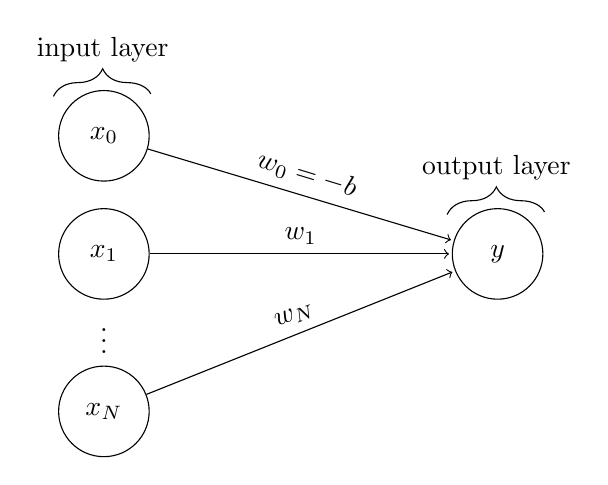
\begin{tikzpicture}[shorten >=1pt]
  	\tikzstyle{unit}=[draw,shape=circle,minimum size=1.15cm]
  	
  	\node[unit](x0) at (0,3.5){$x_0$};
  	\node[unit](x1) at (0,2){$x_1$};
  	\node(dots) at (0,1){\vdots};
  	\node[unit](xn) at (0,0){$x_N$};
  	
  	\node[unit](y1) at (5,2){$y$};
%  	\node(dots) at (4,1.5){\vdots};
%  	\node[unit](yk) at (4,0.5){$y_K$};
  	
  	\draw[->] (x0) -- node[above, rotate = -17]{\( w_0 = -b \)} (y1);
%  	\draw[->] (x0) -- (yk);
  	
  	\draw[->] (x1) -- node[above]{\( w_1 \)}(y1);
%  	\draw[->] (x1) -- (yk);
  	
  	\draw[->] (xn) -- node[above, rotate = 20]{\( w_N \)}(y1);
%  	\draw[->] (xn) -- (yk);
  	
  	\draw [decorate,decoration={brace,amplitude=10pt},xshift=-4pt,yshift=0pt] (-0.5,4) -- (0.75,4) node [black,midway,yshift=+0.6cm]{input layer};
  	\draw [decorate,decoration={brace,amplitude=10pt},xshift=-4pt,yshift=0pt] (4.5,2.5) -- (5.75,2.5) node [black,midway,yshift=+0.6cm]{output layer};
  	\end{tikzpicture}
  	\caption[Network graph of a perceptron with $N$ input units.]{The perceptron consists of $N$ input units and at least one output unit. All units are labeled according to their output: $y = H(z)$ in the case of the output unit; $x_n$ in the case of input units. The input values $x_n$ are propagated to the output unit using a weighted sum, in other words \( z = \bm w^{\intercal}\bm x \). An additional input value $x_0 := 1$ is used to include the biases as weights.}
  	\label{fig:perceptron}
\end{figure}

To describe this more precisely, let $\bm{X}=\{\bm x_n\}_{n=1}^{N}$ be the data, and \( \bm{T} =\{t_n\}_{n=1}^{N},\; t_n\in \{0,1\} \;\forall n \) be the labels. We will refer to the points \( \{(x^n,t^n)\}\subset\bm{X}\times \bm{T} \) as the training set. Then the perceptron algorithm seeks to determine the class of a new data point \( \bm x \) by using a function of the form
\begin{equation}\label{perceptron}
y = H(\bm w^{\intercal} \bm x).
\end{equation}
Here \( \bm w \) is a vector of real weights determined through training and  \( H(v) \) is the Heaviside step function
\[ H(v) =\begin{cases}
 			1 &\text{ if }v\geq 0\\
 			0 &\text{ if }v<0
		 \end{cases} 
\]

In practice, a bias term \( b \) is added to equation \ref{perceptron}, so that it becomes \( y = H(\bm w^{\intercal} \bm x +b) \). This is most usually done by adding an extra feature to all of our data points while training. This extra feature is always set to 1.  An additional weight is also appended to the weight vector \( \bm w \) so that the model still looks like \ref{perceptron}. The effect of bias is to change where the perceptron activates, and makes it harder to `fire' (\textit{i.e.} give a positive output for a given input). This also has the effect of allowing the model to center the data, as would happen with a bias in the regression setting.

%talk a bout finding weight vis gradient descent, this is easier w/ smooth activation lead into logit
The act of training for a perceptron is choosing weights \( \bm w \) so that \( H(\bm w^{\intercal} \bm x_n) = t_n\;\forall (x_n,t_n)\in \mathcal{X}\times \mathcal{T} \). The hope is that this will generalize well to data points not seen in the training set.  The point emphasized in the Minsky book \cite{Minsky90Perceptron} is that training will only work if the two classes in the training set are linearly separable.  This only applies to single layer perceptrons, as one can create a NAND gate from a single layer perceptron, so using multiple perceptrons one could conceivably approximate any function to arbitrary precision.

%single layr as logit regression
%\subsection{Single Layer Network as Logistic Regression}
The perceptron algorithm also includes methods for training, but these are not in common use today.  More modern architecture use the backpropagation algorithm, which requires gradient descent.  The problem with perceptrons in that context is that the derivative of the Heaviside step function is zero. 

The use of the Heaviside function in the perceptron is called an activation function.  In more modern neural networks, activation functions with non-zero derivative allow use of backpropagation and gradient descent.  The discussion in section \ref{logisticReg} mentions the sigmoidal activation function.  As discussed there, if we replace the Heaviside step function with the sigmoid function, then we are actually performing logistic regression.  We will refer to perceptrons using the sigmoidal activation function as sigmoidal neurons.

%multi-layer multiclass network
\subsection{Multilayer Perceptron as a Multi-Class Classifier}
The multilayer perceptron (MLP) is actually built out of several sigmoidal neurons.  The MLP we describe has a single hidden layer, which means that the output of one sigmoidal neuron becomes the input for the next neuron.  Figure \ref{fig:MLP} below gives an example of a single hidden layer MLP.

\begin{figure}[ht]
	\centering
	\begin{tikzpicture}[shorten >=1pt,->,draw=black!50, node distance=\layersep]
	\tikzstyle{every pin edge}=[<-,shorten <=1pt]
	\tikzstyle{neuron}=[circle,fill=black!25,minimum size=17pt,inner sep=0pt]
	\tikzstyle{input neuron}=[neuron, fill=green!20];
	\tikzstyle{output neuron}=[neuron, fill=red!20];
	\tikzstyle{hidden neuron}=[neuron, fill=blue!20];
	\tikzstyle{annot} = [text width=4em, text centered]
	
	% Draw the input layer nodes
	\foreach \name / \y in {1,...,5}
	% This is the same as writing \foreach \name / \y in {1/1,2/2,3/3,4/4}
	\node[input neuron] (I-\name) at (0,-\y) {\(x_\y\)};
	
	% Draw the hidden layer nodes
	\foreach \name / \y in {1,...,6}
	\path[yshift=0.5cm]
	node[hidden neuron] (H-\name) at (\layersep,-\y cm) {\(z_\y\)};
	
	% Draw the output layer nodes
	\foreach \name / \y in {1,...,3}
		\node[output neuron,pin={[pin edge={->}]right:\(\hat{y}_\y\)}] (O-\name) at (2*\layersep,-1 cm-\y cm) {\(y_\y\)};
	
	% Connect every node in the input layer with every node in the
	% hidden layer.
	\foreach \source in {1,...,5}
	\foreach \dest in {1,...,6}
	\path (I-\source) edge (H-\dest);
	
	% Connect every node in the hidden layer with the output layer
	\foreach \source in {1,...,6}
	\foreach \dest in {1,...,3}
	\path (H-\source) edge (O-\dest);
	
	% Annotate the layers
	\node[annot,above of=H-1, node distance=1cm] (hl) {Hidden layer};
	\node[annot,left of=hl] {Input layer};
	\node[annot,right of=hl] {Output layer};
		
	\end{tikzpicture}
		\caption[Network graph of a multilayer perceptron.]{A graph model of a single hidden layer MLP with 5 inputs, 3 output and 6 hidden layer nodes. The output of each layer is determined by composing a linear map with a nonlinear map. The general form of this nonlinear map is determined at the outset, though it may have trained parameters. The linear map is determined through a set of learned weights.}
	\label{fig:MLP}
\end{figure}

Neural networks such as the MLP are often called feedforward neural networks.  This is because at each stage of computation information is only passed forward toward the output nodes.  The general pattern of feedforward nets is that each node passes a weighted sum of previous nodes through an activation function.  We have already mentioned two activation functions, Heaviside and sigmoidal. Other common activation functions are hyperbolic tangent, rectified linear unit (RELU), and sigmoid linear unit \cite{elfwingSiLU}.

In the case of the MLP, each of the hidden layer nodes work as a sigmoidal neuron \textit{i.e.} \( z_l = \gs(\bm w_{1l}^{\intercal}\bm x) \). Likewise, each of the output layers can be expressed as a sigmoidal neuron, \( y_k = \gs(\bm w_{2k}^{\intercal}\bm z) \). This view is not consistent with a desire to express the output in terms of a probability. This is particularly important if we wish to use the MLP as a multi-class classifier, as we wish to interpret the outputs as \( P(k_n=k|\bm x_n) \).

While each individual output is a log odds in the sense of logistic regression, together we cannot interpret each individual \( y_k \)  as a probability.  In particular, we have no guarantee that \( \sum_k y_k=1 \).  To fix this, we may pass the outputs \( y_k \) through the softmax function \textit{i.e.} 
\begin{equation}\label{MLPsoftmax}
\hat{y}_k = \frac{e^{y_k}}{\sum_{j=1}^{K} e^{y_j}}
\end{equation}

Passing the output through a softmax function has the effect of guaranteeing that \( \sum_k y_k=1 \), but if we are to interpret \( \hat{y}_k \) as a probability, then it must be regarded as a Gibbs distribution.  From a mathematical standpoint this changes the interpretation of \( y_k \) to an approximation of an energy function.  To be consistent with this interpretation, we must be careful in our choice of cost function.  This becomes more apparent when we consider the role of backpropagation in training.

\subsection{Backpropagation}\label{subsect:backprop}
Backpropagation (BP) was modernly popularized as a method for training neural networks by Rumelhart et. al. \cite{rumelhart1986learning} in 1986. Similar training methods had been used earlier, \textit{e.g.} Linnainmaa \cite{Linnainmaa1976}, in the context of optimization. Backpropagation for use in neural network training was first used by Paul Werbos in his 1974 thesis \cite{werbos1994roots}. Brief histories of the development of BP can be found in Griewank \textit{et.al.} \cite{griewank2008deriv}, Schmidhuber \cite{Schmidhuber_2015}, and Goodfellow \textit{et.al.},\cite[see ch6.6]{Goodfellow-et-al-2016}. The practical development and popularization of BP led to a very active period of research in multilayer neural networks.

While BP is often described as `just gradient descent', it is the case that BP actually refers to a specific method for calculating the gradient of the loss function with respect to the weights.  Backpropagation relies heavily on the chain rule, and the architecture of perceptron inspired neural networks. We will use a simple neural network model to help describe BP.  We draw most of the inspiration for this example from the book by Goodfellow  et. al. \cite[ch6.5]{Goodfellow-et-al-2016}

The goal of BP is to adjust the weights by subtracting off the gradient of the cost function with respect to the weights.  The key realization of BP is that with the correct network setup, this may be done by passing information backwards through the graph.  

Recall that the typical role of a layer in a feedforward neural net is to pass forward predictions based on information from the previous layer.  The role of layer \( \ell \) during training with backpropagation is to pass forward the predictions as usual. Then during the backward pass layer \( \ell \) updates its own weights \( W_{\ell} \) using gradient descent and the chain rule. Finally the layer passes back the new gradient of the loss with respect to the output \( \bm z_{\ell-1} \)of the previous layer.  Figure \ref{fig:backprop} gives a high level model of this process.

\begin{figure}[ht]
	\centering

%\usetikzlibrary{arrows}
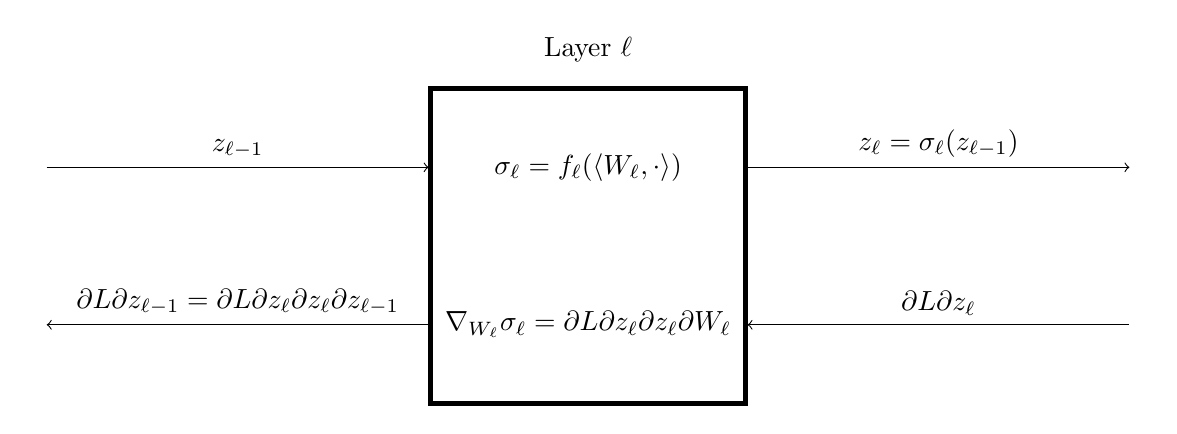
\begin{tikzpicture}

\draw [ultra thick] (-2.5,2.5) rectangle (1.5,-1.5);
\node (v1) at (-7.5,1.5) {};
\node (v2) at (-2.4,1.5) {};
\node (v4) at (-2.4,-0.5) {};
\node (v3) at (-7.5,-0.5) {};
\node (v5) at (1.4,1.5) {};
\node (v6) at (6.5,1.5) {};
\node (v8) at (6.5,-0.5) {};
\node (v7) at (1.4,-0.5) {};
\draw  [->](v1) edge node[above]{\(\bm z_{\ell-1}\)}(v2);
\draw  [<-](v3) edge node[above]{\(\dfrac{\partial L}{\partial \bm z_{\ell-1}}=\dfrac{\partial L}{\partial \bm z_{\ell}}\dfrac{\partial \bm z_{\ell}}{\partial \bm z_{\ell-1}}\)}(v4);
\draw  [->](v5) edge node[above]{\(\bm z_{\ell} = \bm \sigma_{\ell}(\bm z_{\ell-1})\)}(v6);
\draw  [<-](v7) edge node[above]{\(\dfrac{\partial L}{\partial \bm z_{\ell}}\)}(v8);
\node at (-0.5,1.5) {\(\sigma_{\ell} = \bm f_{\ell}(\langle \bm W_{\ell}, \cdot \rangle)\)};
\node at (-0.5,-0.5) {\(\nabla_{\bm W_{\ell}}\sigma_{\ell} = \dfrac{\partial L}{\partial \bm z_{\ell}}\dfrac{\partial \bm z_{\ell}}{\partial \bm W_{\ell}}\)};
\node at (-0.5,3) {Layer $\ell$};
\end{tikzpicture}
	\caption[Conceptualized model of a single network layer.]{A model of a single layer in a neural network. For the feedforward pass it calculates  \(\bm z_{\ell} = \bm \sigma_{\ell}(\bm z_{\ell-1}) = \bm f_{\ell}(\langle \bm W_{\ell},\bm z_{\ell-1}\rangle) \).  On the backward pass it calculates \( \dfrac{\partial L}{\partial \bm W_{\ell}} \) and \( \dfrac{\partial L}{\partial \bm z_{\ell-1}} \). The layer uses \( \dfrac{\partial L}{\partial \bm W_{\ell}} \) to update its own weights with gradient descent. The layer passes \( \dfrac{\partial L}{\partial \bm z_{\ell-1}} \) to the previous layer to use.}
	
\label{fig:backprop}
\end{figure}

While the diagram in figure \ref{fig:backprop} implies that the backpropagation algorithm only uses chain rule, in reality it may be a bit more complicated.  Since \( \gs_{\ell}:\R^{d_{\ell-1}}\rightarrow \R^{d_{\ell}}\) is a non linear multivariate function, taking derivatives can be complicated.  Further, the parameters \( \bm W_{\ell} \) might be part of a higher dimensional linear map (e.g matrix, tensor). For such situations we need to be more careful in calculating gradients.  While many references address this problem, \cite{matGradChain} offers a good treatment of the chain rule in such situations. Section \ref{subsect:derivNotation} covers this in more detail.

Finally it is worth noting that in many situations, backpropagation can be simply calculated in a coordinate manner.  This is because much of the structure of neural nets gives an implied coordinate system to each layer.  It is also a good reason that one must be careful in the choice of cost function. When an appropriate cost function is chosen, backpropagation becomes a quick operation. This helps explain why backpropagation is so popular in recent neural net training.
		\subsection{Derivative Notation}\label{subsect:derivNotation}

Before backpropagation resurfaces in chapter \ref{respLayer}, this section establishes important notation standards.  In the literature \cite{abraham1967transversal, manton2012differential, magnus1985matrix, matGradChain} there are several different notations used for differentiation of functions \( f:\R^n\rightarrow \R^m \). Each author seems to prefer their own notation, and while these notations often overlap, reading various papers quickly becomes confusing without precise communication. This section seeks to establish a reference for derivative notation to be used through the remainder of chapter \ref{respLayer}.

In \citep{patternnet}, care is taken to distinguish the Frech\'et (or contravariant) derivative of a function from the gradient (or covariant derivative) of the same function. Given a vector valued function \( f:\R^n\rightarrow\R^m \), the Frech\'et derivative of \( f \) at \(x\) is the linear map \( A_{ f(x)}:\R^n\rightarrow\R^m \) defined by
\begin{equation}\label{eqn:frechetDefn}
	\lim_{\norm{\bm h}\rightarrow 0} \frac{\norm{f(\bm x+\bm h)-f(\bm x)-A_{f(x)}(\bm h)}}{\norm{\bm h}}=0.
\end{equation}
Provided such a map exists, it is unique.  In particular if \( n,m<\oo \), and \( \pdv{f}{\bm x} = \left(\pdv{f_i}{x_j}\right)_i^j \) is the matrix of partial derivatives (or Jacobian matrix) of \( f \), then \( A_{f(x_0)}(h) = \eval{\pdv{f}{\bm x}}{x_0}\cdot h \).  It is worth noting that the existence of a continuous Jacobian matrix for \( f \) guarantees \( f \) has a Frech\'et derivative.  The reverse implication is not true, \( f \) can have a Frech\'et derivative but not have continuous partials everywhere.

The Frech\'et derivative of \( f \) at the point \( \bm x\in \R^n \) is often denoted by \( Df(\bm x) \), a convention which this dissertation will follow.  The notation \( Df(\bm x)[\bm h] \) works when necessary to discuss both the point \( \bm x \) at which the derivative is being taken, and the direction \( \bm h \) on which it is acting. In this sense it may be said that \( Df \) is a map \( Df:\R^n\rightarrow L(\R^n,\R^m)\). Here, \( L(V,W) \) is the collection of all linear maps from one real vector space \( V \) to another real vector space \( W \).  

Given this notation for the Frech\'et derivative, denote by \( \nabla f(\bm x) \) the gradient of \( f \). A function \( f:\R^n\rightarrow \R^m \) only has a gradient if \( m = 1 \). In this case the gradient is a map \( \nabla f:\R^n\rightarrow\R^n \)such that for all \( \bm x, \bm h \in \R^n \)
\begin{equation}\label{eqn:gradDef}
 Df(\bm x)[\bm h] = \<\bm h, \nabla f(\bm x)\>.
\end{equation} 
Here the angle brackets denote the standard euclidean inner product on \( \R^n \).  Because the gradient of a scalar valued function is a vector valued map, it is possible for \( \nabla f \) to be differentiable. In this case the resulting derivative is called the \textit{Hessian} of \( f \) and will be denoted by \( \nabla^2 f. \) 

An analog of the gradient for functions \( f:\R^n\rightarrow\R^m \) with \( m\geq 1 \) is the adjoint operator of \( Df \). The adjoint operator of any linear map \( A\in L(\R^n,\R^m) \) is the map \( A^{\ast}\in L(\R^m,\R^n) \) such that \( \forall\; x\in\R^n,\) \(y\in\R^m, \) 
\[ \<A(x),y\>_{\R^m} = \<x,A^{\ast}(y)\>_{\R^n}. \]
Since \( Df:\R^n\rightarrow L(\R^n,\R^m) \), the definition of an adjoint operator \( D^{\ast}f:\R^n\rightarrow L(\R^m,R^n)\) depends on the point \( x\in\R^n \) at which it is evaluated.  Thus \( D^{\ast}f \) is defined by 
\begin{equation*}
\<Df(x)[h],u\>_{\R^m} = \<h,D^{\ast}f(x)[u]\>_{\R^n}
\end{equation*}
holding \( \forall\; x,h\in\R^n,\) \(y\in\R^m.\) Aside from the reliance of the definition on the inner product, the adjoint derivative 

When dealing with linear maps between \( \R^n \) and \( \R^m \), all the maps can be recognized as matrix maps; in this case the adjoint is the transpose of the matrix, \textit{i.e.} \( A^\ast = A^{\intercal} \). This is not true for general vector spaces \( V,W \) over \( \R \) as there may be linear maps which cannot be recognized as matrices. An important example is when \( V,W \) are matrix algebras over \( \R \).

Thus it will not be assumed \textit{a priori} that the derivative maps \( Df,\;D^{\ast}f \) are matrix maps.  In fact, for some of the functions used in chapter \ref{respLayer}, \( Df,\;D^{\ast}f \) will not just be linear maps, but multilinear maps, or tensors.  In this case there are still analogs of adjoint operators but more care must be taken in describing them. Discussion of such details will come when necessary.

Since backpropagation does gradient descent, it must calculate the gradient of the loss $L$ with respect to weights $W$. In figure \ref{fig:backprop}, this is shown to be done via the chain rule, but in the general case more care must be applied. The following lemma makes this much easier.
\begin{lemm}\label{gradChain}
	Let $U,V$ be real Riemannian Manifolds and $f:V\rightarrow \R$ and $g:U\rightarrow V$ be smooth maps.  Then if $h=f\circ g$, we have that 
	\[\nabla h=D^{\ast}g[\nabla f\circ g]\]
	where $\nabla h,\nabla f$ are the gradients of $h$ and $f$ respectively, and $D^{\ast}g$ represents the adjoint linear operator of $Dg$ with respect to the metrics on $TV$ and $TU$.
\end{lemm}
\begin{proof}
	This is lemma 4.1 of Theis \citep{matGradChain}. This proof adapts it for use in this dissertation. 
	
	First, let $u \in U$ and $x\in T_uU$ be arbitrary. Because $f,g$ are smooth, they induce maps $Dg(u):T_uU\rightarrow T_{g(u)}V$ and $Df(g(u)):T_{g(u)}V\rightarrow \R$.
	It is given (by definition) that $Dh(u)[x]=\langle \nabla h(u),x\rangle_{T_uU}$. Further, it is clear that $Dh(u):T_uU\rightarrow\R$ is given by $Dh(u)[x]=D(f\circ g)(u)[x]=Df(g(u))[Dg(u)[x]]$. 
	
	Now $Df(g(u))[Dg(u)[x]]=\langle\nabla f(g(u)),Dg(u)[x]\rangle_{T_{g(u)}V}$.  Then for the linear operator $Dg(u):T_uU\rightarrow T_{g(u)}V$, the adjoint linear operator $D^{\ast}g$ is defined by the equation $\langle y,Dg(u)[x]\rangle_{T_{g(u)}V}=\langle D^{\ast}g(u)[y],x\rangle_{T_uU}$ for $x\in T_uU$ and $y\in T_{g(u)}U$.  This gives  
	\[Df(g(u))[Dg(u)[x]]=\langle\nabla f(g(u)),Dg(u)[x]\rangle_{T_{g(u)}V}=\langle D^{\ast}g(u)[\nabla f(g(u))],x\rangle_{T_uU}.\]
	So that $\langle \nabla h(u),x\rangle_{T_uU}=\langle D^{\ast}g(u)[\nabla f(g(u))],x\rangle_{T_uU}$, and as $u,x$ were arbitrary, the theorem is proved.
\end{proof}

A key aspect of the proof above is the use of the metric on $U$ and $V$. This allows identification of tangent spaces to their duals, $TU\cong TU^{*}$ and  $TV\cong TV^{*}$, to define $Dg^{*}$ appropriately. this is not surprising as the definition for the gradient of \( f \) in equation \ref{eqn:gradDef} is closely tied to the inner product on the domain of \( f \).  It follows that wherever derivatives will be used in this dissertation, the appropriate choice of metric (and thus inner product) on the tangent space will be essential. 

%  It may be worth mentioning information geometry and natural gradient descent here. \textcolor{red}{(Fix Later)}. NOPE! 5/11/2020 this is something for a future paper.
Because all the spaces involved can be embedded in \( \R^n \) for some \( n \), many calculations in chapters \ref{Algorithm} and \ref{respLayer} use the inner product on $\bm M=L(\R^N,\R^K)$, defined by the Frobenius inner product $\langle A,B\rangle=\op{tr}(A^{\intercal}\cdot B)$. The map $\op{vec}:\bm M\rightarrow \R^{KN}$ given by stacking the columns of $M$ is a diffeomorphism, and the Frobenius inner product on $\bm M$ is equivalent to the standard euclidean inner product on $\R^{KN}$.  In short, the following diagram commutes.

\begin{equation}\label{eqn:vecfrobcommute}
\begin{tikzcd}
\bm M\times \bm M \arrow[dr, "\op{Frob}" left] \arrow[r, "\op{vec}" above] & \R^{KN}\times \R^{KN} \arrow[d, "\op{euc}" right]\\
[1em] & \R
\end{tikzcd}
\end{equation}
Here $\op{Frob}$ and $\op{euc}$ represent the inner product (metric) on each of the spaces.  

Finally, it is worth mentioning that when necessary, such as in the proof of lemma \ref{gradChain}, discussions reference the tangent space \( TU \) of a Riemannian manifold \( U \).  Since all the spaces here are generally euclidean, such notational references help distinguish the space \( U \) from \( T_uU \), vectors tangent to some point \( u\in U \). The full strength of considering these spaces as manifolds will not be used.
%\Ryan{Talk about what each of these are and their relation to the set of partials.  Mention that for maps from Rm to Rn these are pretty straightforward for the first derivative.  For higher order derivatives it gets messy (tensors). This is also true for maps from matrix spaces to matrix space, but the vec map can turn it into the other situation.  Ultimate goal of chapter: find a vectorized algorithm for computing \( \pdv{L}{F} = \pdv{L}{Y}\pdv{Y}{F} \). If these are both tensors, order matters!}
	\section{Responsible Clustering Algorithms}
		%!TEX root = ../Dissertation_RC.tex

\subsection{$K$-means algorithm}\label{kmeans}
The $K$-means algorithm has been in use for several decades.  Though the first 
mention of the algorithm by name was given by MacQueen in 1967 \cite{
macqueen1967kmeans} the idea had been around for some time.  The standard  
algorithm was used at Bell Labs in 1957 \cite{Lloyd82} for pulse code 
modulation.  Pollard \cite{pollard1981,pollard1982} showed that the $K$-means 
algorithm is consistent in a very precise sense.  Today the algorithm is used 
in many applications \cite{AutoClass1,AutoClass2}, and can be found in many 
good books on machine learning.
\cite{Bishop1995,MacKay2002,BishopBook,hastie09esl,MML_2019}

The outline below is primarily compiled from chapters 20 and 22 of MacKay
\cite{MacKay2002}, though the Bishop and Deisenroth books 
\cite{BishopBook,MML_2019} played a big role.  

The \(K\)-means algorithm is used for vector quantization and for data 
clustering.  It is so named because it separates data points into $K$ distinct 
groups, each characterized by a `mean' \(\bm m_k,\, k= 1,\ldots,K\).  In the 
case that the \(K\)-means algorithm is being used for clustering, these means 
are the cluster centers and each data point is assigned to the closest mean.
In this situation it is the case that 
\[\bm m_k = \frac{\sum_{n=1}^{N} r_k^n \bm x^{(n)}}{N_k}\]
where 
\begin{equation*}
r^n_k = \begin{cases}
			1 & \text{if } \bm x^{(n)} \text{ is closest to } \bm m_k\\
			0 & \text{otherwise}
		\end{cases}
\end{equation*}
and \(N_k = \sum_{n=1}^{N} r^n_k\).  In other words, the means \(\bm m_k\) are 
literally the means of the assignment clusters.

Of course we cannot understand `closest' without first defining a distance 
function  on the underlying data space.  For the original \(K\)-means 
algorithm, the distance was the manhattan distance, though we will use a 
scaled square of the euclidean distance:
\[d(\bm x, \bm y) = \frac 12 \sum_i (x_i-y_i)^2.\]
It is worth noting that the choice of distance in this sense is somewhat 
arbitrary. In most descriptions of the algorithm, euclidean distance is used 
to aid visualization.

To implement the \(K\)-means algorithm, start with \(K\) distinct means.  
A common practice is to use randomly sampled data points 
\(\{\bm m_1 = \bm x^{(n_1)},\ldots,\bm m_K = \bm x^{(n_K)}\}\). Then iteratively 
do the following:
\begin{enumerate}
	\item For each data point, \(\bm x^{(n)}\), set 
	\(\hat{k}_n = \argmin_k d(\bm x^{(n)},\bm m_k)\).
	\item Set \(r_{\hat{k}_n}^{n} = 1\), for each \(n\). Set all other 
	\(r_k^n = 0\)
	\item Calculate \(N_k = \sum_{n=1}^{N} r^n_k\) and 
	\[\bm m_k^{new} = \frac{\sum_{n=1}^{N} r_k^n \bm x^{(n)}}{N_k}.\]
	If \(N_k = 0\), \(\bm m_k^{new} = \bm m_k\).
	\item If \(d(\bm m_k ,\bm m_k^{new})\) is within a predefined tolerance, 
	stop.  Otherwise set \(\bm m_k = \bm m_k^{new}\) and repeat at step 1.
\end{enumerate}
%algorithm? soft k means? generalized k means?
In the literature, it is common to see steps one and two listed as the 
assignment step, and steps three and four as the update step.  

The easiest way to see that this algorithm terminates is to recognize that the 
function \[L := \sum_{n=1}^{N} d(\bm x^{(n)},\bm m_{\hat{k}_n})\]
either stays the same or decreases at each update step.  In this sense, \(L\) 
acts as a Lyapunov function for the \(K\)-means algorithm.

One problem with k-means clustering that is particularly relevant to this 
paper comes when the clusters do not have equal representation in the data.
as an example:\textcolor{red}{(input example)}

In this case, the cluster means are often slightly off center and some data 
points are be inappropriately labeled. %voronoi diagrams? 
One way to fix this is with \textit{soft responsibility}. 
\[r_k^{(n)} = \frac{\exp(-\gb d(\bm x^{(n)},\bm m_k))}
{\sum_i \exp(-\gb d(\bm x^{(n)},\bm m_i))}\]

The idea behind soft responsibility is that each cluster center is partially 
responsible for each data point.  The amount of responsibility \(r_k^{(n)}\) 
of \(\bm m_k\) for the data point \(\bm x^{(n)}\) ought to be inversly 
proportional to \(d(\bm x^{(n)},\bm m_k)\). That is, cluster centers closer to 
data points have greater responsibility for those data points.  

The factor \(\gb\) included here is an inverse temperature, or stiffness 
algorithm, and it can be set at the beginning or iteratively.  In futher 
refinements of the soft $K$-means algorithm, each cluster center has its own
\(\gb_k\), and at each iteration \(\gb_k = \dfrac{1}{\gs_k^2}\) where 
\(\gs_k^{2}\) is the weighted sample variance of the data points assigned to 
cluster $k$.
\[\gs_k^{2} = \frac{\sum_n r_k^{(n)}d(\bm x^{(n)},\bm m_k)}{N_k}\]

Further refinements to this algorithm can be found in MacKay's book, and were 
also developed in the software AutoClass. \cite{MacKay2002,AutoClass1,AutoClass2}

		%!TEX root = ../Dissertation_RC.tex

\subsection{Expectation Maximization} \label{emAlg}
Upon close inspection, it can be seen that the soft \(K\) means algorithm is 
very similar to the Expectation Maximization (or EM) algorithm for Gaussian 
Mixture Models.  What follows is a brief overview of expectation maximization
and the relation of this algorithm to responsibility as discussed in section 
\ref{kmeans}. The discussion below roughly follows discussions available in 
Bishop and other sources \cite{MML_2019, BishopBook, hastie09esl}.

EM was first described in a paper by Dempster et. al. \cite{Dempster77EM}.
The basic idea behind EM is to add hidden or latent variables to a modeling
problem in such a way that maximum likelihood estimation is made easier.  The 
heuristic of this approach is that the latent variables are simply unobserved 
features of the data.  

To be more precise, suppose we are given data $ x $ and we want to fit a model 
with parameters $ \gt $ for the pdf \( p(x|\gt) \) using maximum likelihood 
estimation. In many cases this is an intractable problem that can be simplified
by considering the conditional pdf
\begin{equation}\label{emcond}	
p(x|\gt,z).
\end{equation}

Now as \( z \) are latent variables, we must place a prior \( p(z) \) on the 
distribution of \( z. \) Using \ref{emcond}, and the law of total probability 
we may write
\begin{equation}\label{emtotprob}
p(x|\gt)=\int_{\mathcal{Z}} p(x|\gt,z)p(z)\;dz.
\end{equation}
Where the integral is taken over the space of possible latent variables.

In practice, the integral in \ref{emtotprob} can easily diverge.  The trick is
to choose \( z \) and \( p(z) \) in a manner that avoids this difficulty. 
The EM algorithm is an iterative

%One simplification used for clustering is the assumption that \( z \) is discrete.
%Even if \( z \) is not discrete, we may use Bayes rule to update the prior 
%\(p(z)\).

	\section{Clustering with Mixture Models}
		\section{Mixtures in general}\label{sec1}
 While humans can quickly pick out patterns for data that can be easily visualized, the problems of evaluating high dimensional data, teaching computers to do what humans do easily (e.g.: character recognition), or even of finding new and unknown patterns are interesting from a mathematical perspective.  We will discuss some of the known clustering algorithms available and include some examples of interest.  Examples of interest may include data sets where a given algorithm does especially well, and will include ones where the algorithms work very poorly.
 
In some sense, Clustering may be considered an example of distribution inference given data.  If we have several samples, and a good idea that each sample comes form a different distribution, we can ask two different, but related questions.  First, what are the distributions that were sampled from?  Second, how can we infer which data points came from which distribution? In general, the first question may be called clustering, and the second question classification. For now we will focus mostly on clustering and return to classification later.

To make the question more precise, consider the problem of sampling from $K<\oo$ probability distributions with pdfs \(f_k(x,\gt),\; 1\leq k\leq K\). Each distribution $f_k(x,\gt)$ is chosen at random with proportion $\pi_k^\ast$, $\sum_k \pi_k^\ast=1$.  This is a situation that is mimicked easily enough in Monte Carlo simulations, and is common in applications.  As a two stage experiment, we work as follows to select a point in $x_n\in\R^I$:
\begin{enumerate}
\item Stage 1: From the $K$ possible distributions, select a label $k_n$ with probability $P(k_n=k)=\pi_{k}^\ast$.
\item Stage 2: Sample $x_n$ from $f_{k_n}(x)$
\end{enumerate}

Given $N$ such data points, $D=\{x_n\}_{n=1}^{N}$, clustering then is the problem of estimating the parameters $\gt=\{\bm\pi^\ast,\ldots\}$, where $\bm\pi^\ast\defined\{\pi_k^\ast\}_{k=1}^{K}$. This essentially assigns each of the data points $\bm x_n$ as a sample from a particular pdf in \(f_k(x,\gt),\; 1\leq k\leq K\).  We have in this case 
\[P(x_n|\gt)=\sum_k P(x_n|k_n=k,\gt) P(k_n=k, \gt)=\sum_k \pi_k^\ast f_k(x_n,\gt).\]

One reason that we choose to estimate the parameters $\{\pi_k^\ast\}$ first is that often our other estimates for the remaining parameters $\gt$ are not independent of our choices for the labels.  We proceed as inspired by \textit{Information Theory, Inference, and Learning Algorithms}\citep{MacKay2002}.

Using Bayes' rule, we may formulate a strategy for recovering the parameters $\{p_k\}_{k=1}^{K}$. Given the data $D$, we ask what is the likelihood that the labels chosen were $\{k_n\}_{n=1}^{N}$, given some prior distribution of the labels as $\{\pi_k\}_{k=1}^{K}$. That is to say that $P(k_n=k, \gt)=\pi_k$, for example the naive assumption would be $\pi_k=\frac 1K$.

Bayes rule gives:
\begin{align}\label{Bayes1}
P(k_n=k|\{x_n\},\{\pi_k\})&=\frac{P(x_n|k_n=k)P(k_n=k)}{\sum_{k'}P(x_n|k_n=k')P(k_n=k')} \nonumber \\
						  &=\frac{\pi_k f_k(x_n)}{\sum_{k'}\pi_{k'} f_{k'}(x_n)}
\end{align}

%For a more visual example, consider the ``stacked" functions $f_k$:
%\begin{center}
%%TODO fix the grapics here, probably through a relevant MATLAB example.
%%\includegraphics[scale=.2]{piecewise4.png} 
%	\begin{tikzpicture}[scale=1.75]
%		\draw[->] (-1,0) -- (5,0) node[right] {$x_n$};
%		\draw[->] (0,-.5) -- (0,2.5) node[right] {$P(x_n|\gt)$};
%		\draw[thick,red] plot[samples=100, smooth, domain=-1:5,id=exp1] (\x,{5*exp(-(\x-1)^2/1)/(2*1*sqrt(2*3.14159))});
%		\draw[thick,blue] plot[samples=100, smooth, domain=-1:5,id=exp2] (\x,{5*(exp(-(\x-1)^2/1)/(2*1*sqrt(2*3.14159))+exp(-(\x-2)^2/4)/(4*2*sqrt(2*3.14159)))});
%		\draw[thick,green] plot[samples=100, smooth, domain=-1:5,id=exp3] (\x,{5*(exp(-(\x-1)^2/1)/(2*1*sqrt(2*3.14159))+exp(-(\x-2)^2/4)/(4*2*sqrt(2*3.14159))+exp(-(\x-3)^2/9)/(3*sqrt(2*3.14159)))});
%		\draw[thick] plot[samples=100, smooth, domain=-1:5,id=exp4] (\x,{5*(exp(-(\x-1)^2/1)/(2*1*sqrt(2*3.14159))+exp(-(\x-2)^2/4)/(4*2*sqrt(2*3.14159))+exp(-(\x-3)^2/9)/(3*sqrt(2*3.14159))+exp(-4*(\x-2.5)^2)/(2*1*sqrt(2*3.14159)))});
%		\foreach \x in {-1}
%			\draw[xshift=\x cm] (0pt,2pt) -- (0pt,-2pt) node[below]{$\x$};
%		\foreach \x in {1,...,5}
%			\draw[xshift=\x cm] (0pt,2pt) -- (0pt,-2pt) node[below]{$\x$};
%			
%%		\node [below=1cm, align=flush center,text width=8cm] at (2,-.25)
%%        {
%%           % TODO create graphics here, probably through a relevant MATLAB example.
%%        };
%	\end{tikzpicture}
%\end{center}
%
%In this example, $K=4$, and priors are $\{\pi_k\}_{k=1}^{4}$.  This graphic visualizes the density 
%\[P(x_n|\gt)=\sum \pi_k f_k(x_n)\]
%where the vertical stripe is divided into regions of about $\pi_k f_k(x)$.
%Note here that we have joint distribution which is the mixed discrete-continuous distribution of $(x_n,k_n)$:
%\[P\left(x-\Delta x<x_n<x,k_n=k\right)=\pi_k\cdot\int_{x-\Delta x}^{x}f_k(x_n)\;dx.\]

We have a notion of conditional density
\begin{align*}
\frac{P\left(x-\Delta x<x_n<x,k_n=k\right)}{P\left(x-\Delta x < x_n <x+\Delta x\right)}&\approx\\ \frac{\pi_kf_k(x)\Delta x}{\sum_{k'} \pi_{k'}f_{k'}(x) \Delta x}&=P(x_n|k_n=k,\gt)
\end{align*}

The joint distribution of $\{x_n\}$ and $\{k_n\}$ is 
\[P(\{x_n\}, \{k_n\}|\{\pi_k\})=\prod_n \pi_{k_n}f_{k_n}(x_n).\]
Since we have no practical way of knowing the true labels of points $x_n$; we perform marginalization
\begin{align*}
P(\{x_n\}|\{\pi_k\})&=\sum_{(k_1,k_2,\ldots,k_N)}\prod_n \pi_{k}f_{k_n}(x_n)\\
&= \prod_n \left(\sum_{k}\pi_kf_k(x_n)\right)\\
&= \prod_n P(x_n|\{\pi_k\})
\end{align*}
where $\displaystyle{P(x_n|\{\pi_k\}) =\sum_{k}\pi_kf_k(x_n)}$

\begin{eg} Find the most likely values of $\{\pi_k\}$, given data $\{x_n\}$. We assume complete lack of knowledge, i.e. the prior distribution of $\{\pi_k\}$ is uniform on the standard probability simplex 
\begin{equation}\label{simplexDef}
	S_K:=\left\{\{\pi_k\}_{k=1}^{K}:0\leq \pi_k\leq 1; \sum_{k=1}^{K}\pi_k =1\right\}
\end{equation}

\end{eg}

\begin{soln}
Bayes says
 \[P(\{\pi_k\}|\{x_n\})=\frac{P(\{x_n\}|\{\pi_k\})P(\{\pi_k\})}{\int\int_{\ldots}\int P(\{x_n\}|\{\pi_k\})P(\{\pi_k\})\; d\pi}\]
 Remember that the prior $P(\{\pi_k\})$ is uniform.
\end{soln}
We note here that if we would perform a maximum \textit{a posteriori} estimate at this point, it would be equivalent to finding a maximum likelihood estimator for $\bm\pi^\ast$.

While the marginal probability is difficult to compute, we get a lot of mileage out of looking at the log likelihood.  We define
\begin{align*}
L&:= \ln P(\{x_n\}|\{\pi_k\}) = \sum_n \ln P(x_n|\{\pi_k\})
\end{align*}
and then maximize the likelihood on the simplex $S_K$.
We then define 
\[\{\hat{\pi}_k\}=\argmax_S L\]
The problem of finding the `correct' probability distribution $P(\{\pi_k\})$ then becomes the problem of finding the maximum likelihood estimator of $L$.  

To do this we may use the method of Lagrange multipliers. With our objective function as 
\[\mathcal{L}=L-\gl G\]
where $G(\{\pi_k\})=\sum_k \pi_k -1$, we get the system of equations:
\begin{align*}
&\pder1{\mathcal{L}}{\pi_k}=\pder1{L}{\pi_k}-\gl \pder1{G}{\pi_k}=0\qquad \; k=1,\ldots, K\\
&\pder1{\mathcal{L}}{\gl}=-G(\{\pi_k\})=0
\end{align*}
then we have 
\begin{align*}
\pder1{L}{\pi_k}&=\sum_n \pder1{}{\pi_k}\ln P(x_n|\{\pi_k\})\\
&=\sum_n \frac{f_k(x_n)}{P(x_n|\{\pi_k\})}
\end{align*}
so that the above equations becomes the system of algebraic equations
\begin{align}\label{lageq}
\sum_n\frac{f_k(x_n)}{\sum_{k'}\pi_{k'}f_{k'}(x_n)}&=\gl&k=1,2,\ldots, K\\
\sum_k\pi_k=1
\end{align}

This problem, namely of finding the posterior estimates $\{\hat{\pi}_k\}$ in this manner is well-posed.  We note that in the formation of this problem, we did not incorporate all the conditions of the simplex $S$.  Namely, some of the $\hat{\pi}_k$ could be negative. In practicality this means we need to check the boundary conditions.

%Below is a CAS generated exact solution for $N=2$ data points and $K=2$ clusters.

%TODO generate and insert an example.
	\section{A Brief Introduction to Discrete Dynamical Systems}
		%\Ryan{A \textit{short} section needs to be added here.  Mostly to cover definitions of: stable points, stable sets/manifolds, Lyapunov functions, bifurcations and any other terms unique to dynamical systems and not inference/ML. Marek suggest doing a literature `review', in the sense of citing important theorems.  Maybe a few definitions. }

This section presents some definitions from the field of dynamical systems that are relevant to the dissertation.  Many of these definitions can be found in an undergraduate text like \cite{devaney1989introduction}. The definitions in this section are mostly adapted from the review paper by Mei and Bullo \cite{mei2017lasalle}. Their paper in turn is a summarized version of the contents of a book by LaSalle \cite{lasalle1976dynsys}.

To begin, let \( \N \) represent the natural numbers, and \( \R \) the real numbers. Then \( \R^m \) is \( m \) dimensional euclidean space, and the vectors \( \mathbbm 1_m,\;\bm 0 \) denote the vectors composed entirely of 1's and 0's respectively. The notation \( \bm e_i\;1\leq i\leq m \) will denote the standard basis vectors for \( \R^m \).

For any sequence of points \( \{x_k\}_{k\in\N} \in\R^m\) use \( {x_k}\rightarrow y \) to mean that \( \norm{x_k-y}\rightarrow 0 \) as \( k\rightarrow\oo\). For a set \( S\subset\R^m \), let \( \op{Int}S \) denote the interior of \( S \). If \( S \) is a bounded set, let \( \partial S \) denote the boundary of \( S\), and \( \overbar S = \op{Int}S\cup \partial S\) be the closure of \( S \). The symbol \( \varnothing \) will denote the empty set.  

Given a map \( T:\R^m\rightarrow\R^m \), for \( n\in \N \), define \( T^n=T\circ T\circ\ldots\circ T \) to be the \( n \)-fold composition of \( T \) with itself. The study of \textit{discrete dynamical systems} is, broadly speaking, the study of such continuous maps and their compositions. 

\begin{defn}[Discrete Dynamical System]\label{defn:discDynSys}
	For \( M\subset\R^m \) the map \( \bm\tau:\ZZ\times M\rightarrow M \) describes a discrete dynamical system on \( M \) if for all \( n,k\in\ZZ \) and any \( x\in M \),
	\begin{enumerate}
		\item \(\bm\tau(0,x) = x;\)
		\item \(\bm\tau(n,\bm\tau(k,x)) = \bm\tau(n+k,x)\);\label{eqn:groupProperty}
		\item \( \bm\tau \) is continuous.
	\end{enumerate}
	If requirement \ref{eqn:groupProperty} holds for only \( n,k\geq 0 \), then \( \bm\tau \) describes a discrete \textit{semi-dynamical} system on \( M \). Thus this definition of a discrete dynamical system requires \( \bm\tau(1,x) \) to be a continuous bijection with continuous inverse (\textit{i.e.} a homeomorphism).
\end{defn}

Given a continuous map \( T:M\rightarrow M \) and some initial point \( x_0\in M \), one of the important goals of studying discrete dynamical systems is deciding whether sequences \( \{x_n\}\defined {T^n(x_0)} \) have any limit points.
\begin{defn}[Orbits]
	 Sequences of the form \( x_n = T^n(x_0) \) for some \( x_0 \in M \) are called \textit{orbits} of \(T\).(also motions or trajectories).%\Ryan{Note that motions, trajectories and orbits are actually slightly different things. A motion is a function. Trajectories and orbits are sets. it doesn't hurt to conflate the things for this paper.}
\end{defn} 
Property \ref{eqn:groupProperty} guarantees that for any \( x\in M \), there is exactly one orbit of \(T \) such that \( x_0=x \). By abuse of notation this will be called the orbit of \( x \).

\begin{defn}[Limit points]\label{defn:limitpoints}
	Given a specific point \( x\in M \) the set \( \Omega(x)\subset\R^m \) is the set of all limit points of \( x \). The point \( y\in \R^m \) is a limit point of \( x \) if there is a subsequence \( x_{n_k} \)  with \( |n_k|\rightarrow\oo \) of the orbit \( T^n(x) \) such that \( x_{n_k}\rightarrow y \).  This is the case for both dynamical and semi-dynamical systems. 
\end{defn} 
For some set \( H\subset M \), the set \( \Omega(H) \) is the set of all limit points of for \( x\in H \), \textit{i.e.} \( \Omega(H)=\bigcup_{x\in H}\Omega(x) \). 
\begin{defn}[Invariant Sets]
	The set \( H \) is called \textit{positively invariant} if \( T^n(H)\subset H\;\forall n\in\N \). A set \( H \) is called \textit{negatively invariant} if \( T^n(H)\supset H\;\forall n\in\N \). If \( T(H)=H \) then \( H \) is called \textit{invariant}.
\end{defn} 
A compact invariant set satisfies \( \Omega(H)\subset H \). For discrete semi-dynamical systems, the set \( H \) needs only to be positively invariant and compact.

Property \ref{eqn:groupProperty} is also required to guarantee uniqueness of \textit{periodic points}. \begin{defn}[Periodic points, Fixed points]
	Periodic points are those \( x\in M \) which satisfy \( T^n(x)= x \) for some \( n \).  For a periodic point \(x\), the smallest \( k\in\N \) such that \( T^k(x)=x \) is called the period of \( x \).  \textit{Fixed points} are periodic points of period 1, \textit{i.e.} \( x\in M \) such that \( T(x) = x \).
\end{defn} 
All periodic points of period \( k \) are fixed points of the map \( T^k \). If they exist, periodic points are limit points of a discrete dynamical system.

\begin{defn}[Stable set]
	For a given periodic point \( p\in M \) of period \( k \), the \textit{stable set} of \( p \) is the set of all points \( x\in M \) that eventually arrive at \( p \), \textit{i.e.} \( W^s(T,p)\defined \{x\in M| T^{k+n}(x)\rightarrow p \text{ as } n\rightarrow\oo\}. \)The stable set of a fixed periodic point is always non-empty as it contains \( p \).
\end{defn}  
\begin{defn}[Asymptotically Stable]
	A periodic point \( p \) is called \textit{asymptotically stable} if \( p\in\op{Int}W^s(T,p). \)  In other words, \( p \) is asymptotically stable if there is some \( \gd>0 \) such that \( \norm{x-p}<\gd \) implies that \( T^{k+n}(x)\rightarrow p \), where \( k \) is the period of \( p \).  
\end{defn}

\begin{defn}[Lyapunov stable]
	A point \( x\in M \) is \textit{Lyapunov stable} if points that start sufficiently near \( x \) have orbits close to \( x \). More precisely, \( x \) is Lyapunov stable if for any \( \ge>0\) there is some \(\gd>0\)  such that \( \norm{x-y}<\gd \) implies \( \norm{T^n(x)-T^n(y)}<\ge\) for all \(n\in\N \).
\end{defn}
%\Marek{I don't like the use of quantifiers as if they were verbs in sentences. This is undergraduate-like and quantifiers should be used properly, e.g. they define a variable and its range, and are before the statement that uses the variable. Alternatively, write out ``for all'' and ``there exists''. I find it easier to read, anyway.}\Ryan{agreed, thanks for the comment!}

The last definition of this section is briefly covered in the review paper \cite{mei2017lasalle}, but a more thorough treatment is given by LaSalle in chapter 1 section 6 of \cite{lasalle1976dynsys}. The definition that follows is adapted from LaSalle's work.

\begin{defn}[Lyapunov Function]
	Given a discrete (semi-)dynamical system described by iterating the continuous map \( T:M \rightarrow M\) Let \( G\subset\R^m\), \( G\cap M\neq \varnothing\) then a continuous map \( V:G\rightarrow\R \) is a \textit{Lyapunov function} for \( T \) on \( G \) if \( V(T(x))-V(x)\leq 0 \) for all \( x\in T(M)\cap G \).
\end{defn}

Generally speaking, the map \( V \) is difficult to find for a given discrete dynamical system.  However, as the following theorem shows, very powerful results come from finding a Lyapunov function.

\begin{thm}[Invariance Principle]\label{thm:invariance}\ \\%*[-.2\baselineskip]	
	If \( V \) is a Lyapunov function for \( T \)  on \( G \), define \( E\defined\{\left.x\in\overbar G\right|V(T(x))-V(x)=0\} \) and let \( H \) denote the largest invariant set in \( E \). Then if \( T^n(x)\subset G \) is a bounded orbit of \( x\in G \), there exists a number \( c\in\R \) such that \( T^n(x)\rightarrow H\cap V^{-1}(c) \).
\end{thm}

\begin{proof}
	This is theorem 6.3 of LaSalle chapter 1, section 6 \cite{lasalle1976dynsys}. The same idea is explored in a more general setting in chapter 4 of the same book, and is what allows passage to \( M\subset\R^m \). An accessible, self contained version of the proof can be found in the review paper by Mei and Bullo \cite{mei2017lasalle}.
\end{proof}
\Ryan{Write this as thm 3.1 of chapter 4 in \cite{lasalle1976dynsys}, then cite it in theorem \ref{thm:convergence}.  Maybe put this in an appendix!}
%\Ryan{Maybe a theorem about using lyapunov functions on manifolds with boundary? need lie derivative with the vector field to have constant sign. is there some small set of points where \( -\ell \) is not a lyapunov function? (nope!) Lasalle reference in lyapunov function wikipedia article may be a good book to cite. maybe also lasalle's invariance principle.}
%
%\Ryan{Kantorovich is a better argument, according to Marek. see comments in \ref{sect:expConvRate} for more.}
%		
% add a section about overfitting, generalization, and metrics for performance?
%	\biblio
%\end{document}
% \appendix
% \section{Dynamic Responsibility Code}
\begin{verbatim}
simplex_map.m
stablepoint.m
StablepointNewton.m
GMMData.m
error_samples.m
\end{verbatim}

\section{Responsible Softmax Code}
\begin{verbatim}
RespLoss.m 
FixedRespLoss.m
and dependencies
\end{verbatim}
\section{Code for Examples on GMM Data}
\begin{verbatim}
GMMoverlap.m 
Other data sets?
\end{verbatim}
\section{Code for Example on MNIST Data}
\begin{verbatim}
MNISTBenford.m
\end{verbatim}
%
% \begin{thebibliography}{99}
% And the bibliography goes here.  
% \end{thebibliography}
%
% \end{document}  
% \end{verbatim}
%
% \subsection{The Files and Further Documentation}
%
% Currently, the sources and all documentation are contained in the
% following three files.
% \begin{description}
%
% \item[\texttt{ua-classes.dtx}]
% User guide and documented source code.  The document you are reading has
% been obtained by running |latex ua-classes.dtx|. 
%
% \item[\texttt{ua-classes.ins}]
% The installation file. Running |latex ua-classes.ins| will 
% generate the class  files |ua-thesis.cls| and  |my-thesis.cls| as well
% as the title page packages
% |ua-title.sty| and |my-title.sty| from the universal source file
% |ua-classes.dtx|.
%
% \item[\texttt{ua-example.tex}]
% An example dissertation generated from the official Manual for Theses and
% Dissertations by the Graduate College.  The file has been obtained via
% the web and manually converted into \LaTeX.  It both serves as an example
% and contains the official formating instructions as of May 1996.  Be sure
% to check for changes before you submit your dissertation. 
%
% \end{description}
%
%
% \subsection{Bugs and Changes}
%
% All changes and bug fixes must be done in the file |ua-classes.dtx|,
% and \emph{not} in the files generated by the docstrip utility.  Moreover,
% they must be clearly annotated with a date, name and comments explaining
% each change.
%
%
% \section{The Code}
%
% This section contains a commented listing of the source code.
% It is intended for \TeX perts to facilitate alterations and
% debugging (hopefully the latter will not become necessary).
% 
% \subsection{The Identification Part}
%
%    \begin{macrocode}
\NeedsTeXFormat{LaTeX2e}
%<*ua-thesis>
\ProvidesClass{ua-thesis}
              [1997/03/08 UA Thesis Class]
%</ua-thesis>
%<*my-thesis>              
\ProvidesClass{my-thesis}
              [1997/03/08 My Private Thesis Class]
%</my-thesis>
%<*ua-title>
\ProvidesPackage{ua-title}[1997/03/08]
%</ua-title>
%<*my-title>
\ProvidesPackage{my-title}[1997/03/08]
%</my-title>
%    \end{macrocode}
%
% \subsection{Package Options}
%
% We pass the global package options through to the underlying
% document class.  In the |ua-thesis| class we also keep track of
% whether the |draft| or |final| option is switched on because
% we will link certain document features (see Section 1) to
% this option.
%    \begin{macrocode}
%<*ua-thesis>
\newif\iffinal@
\DeclareOption{final}{%
  \final@true
  \PassOptionsToClass{final}{report}}
\DeclareOption{draft}{%
  \final@false
  \PassOptionsToClass{draft}{report}}
\ExecuteOptions{draft}  
\DeclareOption*{\PassOptionsToClass{\CurrentOption}{report}}
\ProcessOptions
%</ua-thesis>
%    \end{macrocode}
% In the |my-thesis| class, nothing particular happens.
%    \begin{macrocode}
%<*my-thesis>
\DeclareOption*{\PassOptionsToClass{\CurrentOption}{amsbook}}
\ProcessOptions
%</my-thesis>
%    \end{macrocode}
%
% \subsection{The Underlying Document Classes}
%
% The official |ua-thesis| class is based on the standard |report|
% document class.  We load it with the |12pt| option as default,
% which is smallest size allowed.  We have to load the 
% packages of the AMS math bundle explicitly.
% Added 1997/3/8: In fact, even |ua-thesis| breaks with old versions
% of the AMS macros, so we add a release date to |\RequirePackage|.
%    \begin{macrocode}
%<*ua-thesis>
\LoadClass[12pt]{report}
\RequirePackage[reqno]{amsmath}[1996/10/24]
\RequirePackage{amsfonts}[1996/10/24]
\RequirePackage{amsthm}[1996/10/24]
\RequirePackage{ua-title}
%</ua-thesis>
%    \end{macrocode}
% We want the equation numbers on the right, thus the |reqno| option.
%
% The |my-thesis| class is based on the |amsbook| class
% with modifications adopted from the |pcms-l| package, also by the
% AMS.  The packages of the AMS math bundle are loaded by default from
% within |amsbook|.  Added 1996/12/05: The updated version works only
% with the new release of the AMS macros, dated 1996/10/24.
%    \begin{macrocode}
%<*my-thesis>
\LoadClass[reqno]{amsbook}[1996/10/24]
\RequirePackage{my-title}
%</my-thesis>
%    \end{macrocode}
%
% \subsection{General Style Settings for \texttt{ua-thesis}}
%
% Redefine the name of the Table of Contents and the References
% according to the Graduate College regulations.
% We also have to redefine |\listfigurename| and |\listtablename| with
% |\def| (although the names are not changed),
% otherwise they have the wrong status with respect to the \TeX
% internals |\outer| and |\long|, and the |\ifx| statements in the
% |\@chapterstar| macro won't work.
%    \begin{macrocode}
%<*ua-thesis>
\def\contentsname{Table of Contents}
\def\bibname{References}
\def\dedicationname{Dedication}
\def\listfigurename{List of Figures}
\def\listtablename{List of Tables}
%    \end{macrocode}
% Set the page margins as required by the Graduate College: Top margin is
% $1.5$in, bottom margin is $1$in, left margin is $1.5$in and the right
% margin is $1$in.  We grant an extra $0.2$in to the bottom margin to allow
% for printer tolerances and to account for characters that extend below
% the base line (e.g.\ the character ``y'').
%    \begin{macrocode}
\topmargin      0in
\headheight     \baselineskip
\headsep        0.6in
\addtolength{\headsep}{-\headheight}
\footskip       0in
\textheight     \paperheight
\addtolength{\textheight}{-2.7in}
\oddsidemargin  0.5in
\evensidemargin 0.5in
\marginparwidth 0in
\marginparsep   0in
\textwidth      \paperwidth
\addtolength{\textwidth}{-2.5in}
%    \end{macrocode}
% Macros to switch from single-spaced to double-spaced printing.
% The command |\doublespaced| takes only effect when it is used
% with the |final| option.
%    \begin{macrocode}
\def\singlespaced{\baselineskip=\normalbaselineskip}
\def\doublespaced{\iffinal@ \baselineskip=1.5\normalbaselineskip \fi}
%    \end{macrocode}
% Finally, we define the page styles as required.  As we are modifying the
% |\topskip| when typesetting chapter headings and when selecting
% page style |continued|, we save the default value and restore
% it on ``normal'' pages.
%    \begin{macrocode}
\newlength{\@topskipsave}
\@topskipsave\topskip
%    \end{macrocode}
% The page style |topright| is used on normal pages.  It puts
% the page number into the top
% header at the right margin of each page.
%    \begin{macrocode}
\def\ps@topright{%
    \let\@mkboth\@gobbletwo
    \topskip\@topskipsave
    \def\@oddhead{\normalfont\hfil\thepage}
    \let\@evenhead\@oddhead
    \def\@evenfoot{}
    \def\@oddfoot{}}
%    \end{macrocode}
% Page style |continued| is for the second and following pages of
% the Table of Contents, the List of Figures and the List of Tables.
% The macro |\@continued| contains the required heading for those
% pages, e.g.\ ``Table of Contents---Continued''.
%    \begin{macrocode}
\def\ps@continued{%
    \let\@mkboth\@gobbletwo
    \topskip 0.5in
    \def\@oddhead{\raisebox{-0.5in}{\@continued}%
                  \hfil\normalfont\thepage}
    \let\@evenhead\@oddhead
    \def\@evenfoot{}
    \def\@oddfoot{}}
%    \end{macrocode}
% The \TeX\ mechanism for starting pages is rather mysterious.  There is
% some extra space associated with the variable |\topskip|. However, it
% is not sufficient to just set |\topskip| to zero.  One moreover has to
% place a box of zero height onto the page, otherwise \TeX\ inserts extra
% vertical space, and we lose precise control over the placements
% of the layout elements.  The following macro is called whenever a
% title page (main title, chapter title, etc.) is started.
%    \begin{macrocode}
\def\@notopskip{\topskip\z@ \hrule height\z@}
%</ua-thesis>
%    \end{macrocode}
%
% \subsection{Some Style Defaults of the \texttt{my-thesis} Class}
%
% We mostly follow the defaults given by the |amsbook| class, but there
% are few things worth changing.  First we add some space between the items
% of a list---we don't have to be too stingy with vertical space.
% The next four lines are copied from |amsbook.cls| with changed definition
% for |\itemsep|.
%    \begin{macrocode}
%<*my-thesis>
\def\@listI{\leftmargin\leftmargini \parsep\z@skip
  \topsep\listisep \itemsep\topsep
  \listparindent\normalparindent}
\let\@listi\@listI
%    \end{macrocode}
% Moreover, sections are to be numbered within chapters, and we give the
% Abstract the appearance of an unnumbered chapter.
%    \begin{macrocode}
\numberwithin{section}{chapter}
\renewenvironment{abstract}%
  {\chapter*{Abstract}}{}
%    \end{macrocode}
% We must define a bibliography style to avoid an error message.
%    \begin{macrocode}  
\bibliographystyle{amsplain}
%</my-thesis>
%    \end{macrocode}
%
% \subsection{The Title Page Packages}
%
% The title page macros are put into separate files, so that they can
% be used in conjunction with other document classes, if this is
% desirable.
%
% First some common code that defines the macros for
% various layout elements in the title page(s).  The |my-thesis| class
% will not use all of them, but their definition is required anyway to
% assure compatibility with |ua-thesis|. The defaults are set as follows:
%    \begin{macrocode}
%<*ua-title|my-title>
\let\@title\@empty
\let\@author\@empty
\let\@copyright\@empty
\def\@thesis{Dissertation}
\def\@department{Graduate Interdisciplinary Program \\
                 in Applied Mathematics}
\def\@degree{Doctor of Philosophy}
\def\@degreeabbrev{Ph.D.}
\let\@major\@empty
\let\@director\@empty
\let\@directortitle\@empty
%    \end{macrocode}
% In the following, changed |\newcommand| to |\renewcommand|
% because the new release
% of the AMS classes seems to define |\copyrightholder| while the
% old release doesn't (1996/12/05).
%    \begin{macrocode}
\def\copyrightholder#1{\gdef\@copyright{#1}}
\newcommand{\thesis}         [1]{\gdef\@thesis{#1}}
\newcommand{\department}     [1]{\gdef\@department{#1}}
\newcommand{\degree}         [1]{\gdef\@degree{#1}}
\newcommand{\degreeabbrev}   [1]{\gdef\@degreeabbrev{#1}}
\newcommand{\major}          [1]{\gdef\@major{#1}}
\newcommand{\director}       [1]{\gdef\@director{#1}}
\newcommand{\directortitle}  [1]{\gdef\@directortitle{#1}}
%    \end{macrocode}
% We redefine the |\title| and |\author| commands to follow the
% AMS syntax.  The optional
% argument allowed in the AMS classes is simply ignored without
% an error message.
%    \begin{macrocode}
\renewcommand{\title} [2][]{\gdef\@title{#2}}
\renewcommand{\author}[2][]{\gdef\@author{#2}}
%</ua-title|my-title>
%    \end{macrocode}
% 
%
% \subsubsection{The Official Title Page}
% 
% This macro is largely self-explanatory \ldots
%
%    \begin{macrocode}
%<*ua-title>
\def\@SetTitlePage{%
  \thispagestyle{empty}
  \begingroup
    \centering
    \@notopskip
    \vspace*{1in}
    \begingroup
      \Large\scshape
      \addtolength{\baselineskip}{8pt}
      \@title \\
    \endgroup
    \vspace*{\stretch{1}}
    by \\[5pt]
    \@author \\
    \hrule height\z@
    \vspace*{\stretch{2}}
    \begingroup
      \rule{2in}{0.7pt} \\
      \ifx\@empty\@copyright
        \else Copyright \copyright\ \@copyright \\
        \fi
    \endgroup
    \vspace*{\stretch{2}}
    \begingroup
%    \end{macrocode}
% The following line sets the inter-word space to twice its original value.
%    \begin{macrocode}
      \spaceskip1.3\fontdimen2\font plus1.3\fontdimen3\font
      A \@thesis\ Submitted to the Faculty of the \\[8pt]
      \textsc{\large\@department} \\[8pt]
      In Partial Fulfillment of the Requirements \\
      For the Degree of \\[8pt]
      \textsc{\large\@degree}
      \ifx\@empty\@major
         \else \\
               \textsc{\large With a Major in \@major}
         \fi \\[8pt]
      In the Graduate College \\[8pt]
      \textsc{\large The University of Arizona} \\
    \endgroup
    \vspace*{\stretch{1}}
    \spaced{\@date}
    \vspace*{0.5in}
    \newpage
  \endgroup}
%    \end{macrocode}
% To make |\@SetTitlePage| work with standard document classes, we redefine
% |\maketitle| to be |\@SetTitlePage|.  This choice will later be
% overridden by the |ua-thesis| class.
%    \begin{macrocode}
\let\maketitle\@SetTitlePage
%</ua-title>
%    \end{macrocode}
%
%
% \subsubsection{My Title Page}
%
% Here we can simply redefine |\maketitle| directly without the help of
% an auxiliary macro.
%    \begin{macrocode}
%<*my-title>
\def\maketitle{%
  \cleardoublepage
  \thispagestyle{empty}
  \begingroup
    \centering
    \vspace*{\stretch{1}}
    \hrule height 1pt
    \begingroup
      \Huge\bfseries
      \addtolength{\baselineskip}{2pt}
      \medskip
      \@title \\
      \medskip
    \endgroup
    \hrule height 1pt
    \vspace*{\stretch{1}}
    \begingroup
      \huge \@author \\
    \endgroup
    \vspace*{\stretch{1.7}}
    \begingroup
      \Large
      \spaceskip1.3\fontdimen2\font plus1.3\fontdimen3\font
      A \@thesis\ Submitted to the Faculty of the \\[8pt]
      \textsc{\LARGE\@department} \\[8pt]
      In Partial Fulfillment of the Requirements \\
      For the Degree of \\[8pt]
      \textsc{\LARGE\@degree}
      \ifx\@empty\@major
         \else \\
               \textsc{\LARGE With a Major in \@major}
         \fi \\[8pt]
      In the Graduate College \\[8pt]
      \textsc{\LARGE The University of Arizona} \\
    \endgroup
    \vspace*{0.8cm}
    {\Large\spaced{\@date}}
    \newpage
  \endgroup}
%</my-title>
%    \end{macrocode}
%
%
% \subsubsection{Setting the Date with Spaces Between Digits}
% 
% In order to increase the inter-letter space in the date, we resort to
% a technique which is a simplified version of the 
% |letterspace| package (by Philip Taylor, described in The
% \LaTeX\ Companion).  The macro |\spaced| puts spaces between all the
% characters of its argument.  
%    \begin{macrocode}
%<*ua-title|my-title>
\def \spaced #1%
    {\edef \3{#1}%
     {\expandafter \insertsp@ces \3\@nd}%
    }
\def \insertsp@ces #1#2\@nd
    {\def \1{#1}%
     \def \2{#2}%
     \1%
     \ifx \1\empty \else \ifx \2\empty \else \space \fi \fi
     \ifx \2\empty
          \let \n@xt = \relax
     \else
          \futurelet \2\m@kespaceexplicit #2\@nd
          \def \n@xt {\expandafter \insertsp@ces \2\@nd}%
     \fi
     \n@xt
    }
\def \m@kespaceexplicit #1#2\@nd %
    {\if \2 \def \2{{ }#1#2}\else \def \2{#1#2}\fi}
%</ua-title|my-title>
%    \end{macrocode}
%
%
% \subsubsection{Official Approval and Copyright Pages}
%
% This code is specific to the |ua-thesis| class.  Here |\maketitle|
% has to invoke the automatic generation of the Approval and the Copyright
% Page, provided that the |final| option is set. 
%    \begin{macrocode}
%<*ua-thesis>
\def\maketitle{%
  \cleardoublepage
  \begingroup
    \@SetTitlePage
    \iffinal@
      \@SetApprovalForm
      \@SetAuthorStatement
    \fi
  \endgroup
  \let\maketitle\relax}
%    \end{macrocode}
% Make an empty approval page which is eventually to be substituted by
% the official approval page from the Graduate College.  This macro is
% only called if the |final| option is set.
%    \begin{macrocode}
\def\@SetApprovalForm{%
  \pagestyle{topright}
  \@notopskip
  \vspace*{\fill}
  \begin{center}
    \Large
    Get the official approval page \\
    from the Graduate College \\
    \textsl{before} your final defense.
  \end{center}
  \vspace*{\fill}
  \vspace*{0.5in}
  \newpage}
%    \end{macrocode}
% Now the Copyright page.  The copyright page is also printed only
% with the |final| option in place.
%    \begin{macrocode}
\def\@SetAuthorStatement{%
   \begingroup
     \pagestyle{topright}
     \@notopskip
     \vspace*{1in}
     \begingroup
       \centering\large\scshape
       Statement by Author \\
     \endgroup
     \bigskip\bigskip
     \par
     This \MakeLowercase{\@thesis} has been submitted in partial
     fulfillment of requirements for an advanced degree at The
     University of Arizona and is deposited in the University
     Library to be made available to borrowers under rules
     of the Library.
     \bigskip
     \par
     Brief quotations from this \MakeLowercase{\@thesis} are
     allowable without special permission, provided that accurate
     acknowledgment of source is made. Requests for permission for
     extended quotation from or reproduction of this manuscript in
     whole or in part may be granted by the
     \ifx\@empty\@copyright
       head of the major department or the Dean of the Graduate
       College when in his or her judgment the proposed use of
       the material is in the interests of scholarship.
       In all other instances, however,
       permission must be obtained from the author.
     \else
       copyright holder.
     \fi
     \par
     \vspace*{3\baselineskip}
     \begin{flushright}
       \scshape
       Signed: \underline{\makebox[2.5in][r]{}}
     \end{flushright}
     \vspace*{\fill}
     \ifx\@empty\@directortitle
     \else
       \begingroup
          \centering
          \large\scshape
          Approval by \@thesis\ Director
       \endgroup
       \bigskip\bigskip\par
       This \MakeLowercase{\@thesis} has been approved
       on the date shown below:
       \vspace*{3\baselineskip}\par\noindent
       \begin{minipage}[t]{0.45\textwidth}
         \begin{center}
           \underline{\makebox[\textwidth][r]{}} \\
           \@director \\
           \@directortitle
         \end{center}
       \end{minipage}%
       \hfill%
       \begin{minipage}[t]{0.45\textwidth}
         \begin{center}
           \underline{\makebox[\textwidth][r]{}} \\
           Date
         \end{center}
       \end{minipage}
     \fi
     \vspace*{0.5in}
     \newpage
   \endgroup}
%    \end{macrocode}
%
% \subsubsection{Abstract and Special Abstract}
%
% Setting the abstract in the official thesis class
% is tricky.  Since we have to typeset it twice, for
% the regular and the special abstract, and we want to keep the regular
% \LaTeX\ syntax of having an |abstract| environment, we somehow have to 
% save the body of the abstract environment for further processing.
% This is quite difficult to do in \TeX, but fortunately the |amsmath|
% package has solved this problem for us.  It defines the internal macro
% |\collect@body| which takes a single argument, namely the name of
% a macro which does the processing.  This macro is then called by
% |\collect@body|, and given the contents of the environment body as
% its argument.  We redefine these macros here, mainly for the reason that
% we want the auxiliary macros |\collect@@body|
% and |\Addto@envbody| to be defined with
% |\long\def|, so that the abstract can have more than one paragraph.
% We capitalize all macros not to interfere with the |amsmath| package
% (actually, our change would only change |amsmath|s response to
% errors, not its behavior with correct code).
%    \begin{macrocode}
\long\def\Addto@envbody#1{\@envbody\@xp{\the\@envbody#1}}
\def\Collect@body#1{%
    \@envbody{}%
    \def\process@envbody{%
        \@xp#1\@xp{\the\@envbody}%
    }%
    \@xp\let\csname\@currenvir\endcsname\Collect@@body
    \csname\@currenvir\endcsname
}
\long\def\Collect@@body#1\end#2{%
    \def\@tempa{#2}%
    \ifx\@tempa\@currenvir
        \Addto@envbody{#1}%
        \@xp\edef\csname\@currenvir\endcsname{%
            \@nx\process@envbody\@nx\end{\@tempa}%
            }%
    \else
        \Addto@envbody{#1\end{#2}}%
    \fi
    \csname\@currenvir\endcsname
}
%    \end{macrocode}
% The details of the above are explained in |amsmath.dtx|. For us it
% is mainly a convenience, and the remainder of the abstract
% macro can be coded in a very elegant way.
%    \begin{macrocode}
\renewenvironment{abstract}{%
  \Collect@body\@SetAbstract}{}
%    \end{macrocode}
% Now the macro |\@SetAbstract|, which actually does the work. First
% we typeset the regular abstract.
%    \begin{macrocode}
\long\def\@SetAbstract#1{%
  \chapter*{Abstract} 
  #1
  \clearpage
%    \end{macrocode}
% Then the special abstract. We typeset it only in the final version. Note
% that we have to save the page counter at the beginning of the special
% abstract, so that it doesn't interfere with the page numbering of the
% main document.
%    \begin{macrocode}
  \iffinal@
  \begingroup
    \clearpage
    \newcounter{s@avepageno}
    \setcounter{s@avepageno}{\value{page}}
    \setcounter{page}{1}
    \thispagestyle{empty}  
    \@notopskip
    \begingroup
      \centering
      \large\textsc
      \@title \\
      \bigskip
      \normalfont\normalsize
      \@author, \@degreeabbrev \\
      The University of Arizona, \@date \\
    \endgroup
    \bigskip
    \noindent Director: \@director \par
    \bigskip\bigskip
    #1
  \endgroup
  \clearpage
  \setcounter{page}{\value{s@avepageno}}
  \fi}  
%    \end{macrocode}
% 
%
% \subsection{The Sectioning Commands}
%
% \subsubsection{Chapter Headings in the Official Format}
%
% The |\chapter| macro is standard code.  It calls |\@chapter| for
% numbered chapters, and |\@chapterstar| for unnumbered ones.
%    \begin{macrocode}
\def\chapter{%
  \clearpage
  \global\@topnum\z@
  \@afterindentfalse
  \secdef\@chapter\@chapterstar}
%    \end{macrocode}
% For numbered chapters we do all the usual things:  Set the page style in
% case it has been modified previously, increment the chapter counter, 
% create the Table of Contents entry and add extra space into the
% List of Figures and List of Tables.
%    \begin{macrocode}
\def\@chapter[#1]#2{%
  \pagestyle{topright}
  \refstepcounter{chapter}%
  \typeout{\@chapapp \space \thechapter}
  \addcontentsline{toc}{chapter}%
    {\protect\chapterline{\@chapapp\ \thechapter}#1}
  \addtocontents{lof}{\protect\addvspace{\medskipamount}}
  \addtocontents{lot}{\protect\addvspace{\medskipamount}}
%    \end{macrocode}
% Then we typeset the chapter heading.
%    \begin{macrocode}  
  \begingroup
    \@notopskip
    \centering
    \vspace*{0.25in}
    \textbf{\@chapapp\ \thechapter} \\
    \medskip
    \Large\textsc{#2} \par
  \endgroup
  \vspace*{2\normalbaselineskip}
  \@afterheading
  \doublespaced}
%    \end{macrocode}
% Unnumbered chapters are more tricky.  Several explicitly format decisions
% have to be made to typeset all the special ``chapters'' in the
% front matter of the dissertation according to the official requirements.
%
% The following rules are implemented: The Dedication is typeset
% double-spaced.  The Table of Contents, List of Figures and List of Tables
% must be get pagestyle |continued| and be single-spaced.  In all other
% cases pagestyle |topright| is selected.
% Only those unnumbered chapters that
% come after the Table of Contents will get an entry in the Table of
% Contents.  An arbitrary unnumbered chapter that comes after the
% Table of Contents will be double-spaced, the exception is the References,
% which are single-spaced.   If an unnumbered chapter comes before the
% Table of Contents, no explicit decision between single and double-spaced
% is made.  The effect is that the Acknowledgments will be single-spaced,
% provided they are placed in the officially required order.
%    \begin{macrocode}
\def\@chapterstar#1{%
  \typeout{#1}
  \edef\1{#1}
  \ifx \dedicationname\1
       \doublespaced
  \else     
  \ifx \contentsname\1 
       \@specialhead\1
       \singlespaced
       \let\tableofcontents\relax
  \else
  \ifx \listfigurename\1
       \@specialhead\1
       \@tocentry\1
       \singlespaced
  \else
  \ifx \listtablename\1
       \@specialhead\1
       \@tocentry\1
       \singlespaced
  \else
  \pagestyle{topright}
  \ifx \tableofcontents\relax
       \@tocentry\1
       \ifx \bibname\1 \singlespaced \else \doublespaced \fi
  \fi\fi\fi\fi\fi
%    \end{macrocode}
% And this is the code to typeset the heading.
%    \begin{macrocode}  
  \begingroup
    \@notopskip
    \centering
    \Large\textsc{#1} \par
  \endgroup
  \vspace*{2\normalbaselineskip}
  \@afterheading}
%    \end{macrocode}
% The following macro creates the Table of Contents entry for unnumbered
% chapters.
%    \begin{macrocode}
\def\@tocentry#1{%
  \addcontentsline{toc}{chapter}{#1}
  \addtocontents{lof}{\protect\addvspace{\medskipamount}}
  \addtocontents{lof}{\protect\addvspace{\medskipamount}}}
%    \end{macrocode}
% And this one switches to pagestyle |continued| and defines the
% extra part of the page heading.
%    \begin{macrocode}
\def\@specialhead#1{%
  \gdef\@continued{\normalsize\scshape#1---\slshape Continued}
  \pagestyle{continued}
  \thispagestyle{topright}}
%</ua-thesis>
%    \end{macrocode}
%
% \subsubsection{Chapter Headings in the Un-Official Format}
%
% The following code for chapter headings is taken from the
% |pcms-l| class by the AMS.  It is slightly simplified
% because we don't have to deal with different ``lectures'' and
% multiple authors.
%    \begin{macrocode}
%<*my-thesis>
\def\chapter{\cleardoublepage \pagestyle{headings}%
  \setcounter{section}0\relax
  \thispagestyle{plain}%
  \global\@topnum\z@
  \@afterindentfalse \secdef\@chapter\@schapter}
%
\def\@chapter[#1]#2{\refstepcounter{chapter}%
  \ifnum \c@secnumdepth <\z@ \let\thechapter\@empty\fi
  \let\@secnumber\thechapter
  \typeout{\chaptername\space\thechapter}%
  \addcontentsline{toc}{chapter}{%
    \protect\numberline{%
      \ifx\thechapter\@empty\else\chaptername\ \thechapter.\fi}#1}%
  \chaptermark{#1}%
  \addtocontents{lof}{\protect\addvspace{10\p@}}%
  \addtocontents{lot}{\protect\addvspace{10\p@}}%
  \@makechapterhead{#2}\@afterheading}
%
\def\@schapter#1{\typeout{#1}%
  \@ifnotempty{#1}{\addcontentsline{toc}{chapter}{#1}}%
  \let\@secnumber\empty
  \chaptermark{#1}%
  \addtocontents{lof}{\protect\addvspace{10\p@}}%
  \addtocontents{lot}{\protect\addvspace{10\p@}}%
  \@makeschapterhead{#1}\@afterheading}
%    \end{macrocode}
% For typesetting the chapter head we fixed one problem with
% |pcms-l|:  The first |\vspace| was originally achieved
% through modifying |\topskip|.  However, for mysterious reasons,
% the modification is reset to the default whenever floats are defined
% on the first page of a chapter.
%    \begin{macrocode}
\def\@makechapterhead#1{\begingroup 
  \vspace*{37pt}
   \ifodd\c@page\raggedleft\else\raggedright\fi
    \ifnum\c@secnumdepth>\m@ne
      \leavevmode
     {\Large\bfseries
              \uppercase\@xp{\chaptername}\enspace
        {\LARGE\bfseries\thechapter\par}}\skip@34\p@ 
                \advance\skip@-\normalbaselineskip
        \vskip\skip@ {\huge\bfseries #1\par}\fi
 \endgroup
  \skip@34\p@ \advance\skip@-\normalbaselineskip
  \vskip\skip@ }
%    \end{macrocode}
% And the chapter head for unnumbered chapters:
%    \begin{macrocode}
%
\def\@makeschapterhead#1{%
        \vtop to 8pc{\vfill
  \ifodd\c@page\raggedleft\else\raggedright\fi
  {\huge\bfseries #1\par}%
}%\endgroup
\skip@34\p@\advance\skip@-\normalbaselineskip
  \vskip\skip@ }
%</my-thesis>  
%    \end{macrocode}
%
% \subsubsection{Section, Subsections etc.}
%
% Here we follow literally the |pcms-l| settings, both for |ua-thesis| and
% |my-thesis|.  The appearance is similar to the |report| class, but the
% type sizes are scaled down one step, which looks less excessive.
%    \begin{macrocode}
%<*ua-thesis|my-thesis>
\def\section{\@startsection{section}{1}%
  \z@{-1\baselineskip\@plus-.75\baselineskip}{.5\baselineskip}%
  {\large\bfseries}}
%
\def\subsection{\@startsection{subsection}{2}%
  \z@{-.75\baselineskip\@plus-.5\baselineskip}{.5\baselineskip}%
  {\normalfont\bfseries}}
%
\def\subsubsection{\@startsection{subsubsection}{3}%
   \z@{.5\baselineskip\@plus.5\baselineskip}{-5\p@}%
   {\normalfont\itshape}}
%    \end{macrocode}
% The same for the appearance of theorems, remarks, definitions and
% proofs. Directly from |pcms-l|.
%
% Changed on 1996/12/05:
% The following four macros are all
% taken from the October 1996 release from |pcms-l|, because the
% new release of |amsthm| breaks these macros.  No attempt is
% made to be compatible with the old version.
%    \begin{macrocode}
\def\th@plain{%
  \let\thm@indent\noindent
  \thm@headfont{\bfseries}% heading font bold
  \thm@notefont{\mdseries\upshape}
  \thm@preskip.5\baselineskip\@plus.2\baselineskip
                                    \@minus.2\baselineskip
  \thm@postskip\thm@preskip
  \itshape
}
\def\th@remark{%
  \let\thm@indent\noindent
  \thm@headfont{\bfseries}% heading font bold
  \thm@notefont{\mdseries\upshape}%
  \thm@preskip.5\baselineskip\@plus.2\baselineskip
                                    \@minus.2\baselineskip
  \thm@postskip\thm@preskip
  \upshape
}
\def\th@definition{%
  \let\thm@indent\noindent
  \thm@headfont{\bfseries}% heading font bold
  \thm@notefont{\mdseries\upshape}%
  \thm@preskip.5\baselineskip\@plus.2\baselineskip
                                    \@minus.2\baselineskip
  \thm@postskip\thm@preskip
  \upshape
}
\renewenvironment{proof}[1][\proofname]{\par \normalfont
  \topsep6\p@\@plus6\p@ \trivlist \itemindent\z@
  \item[\hskip\labelsep\bfseries
    #1\@addpunct{.}]\ignorespaces
}{%
  \qed\endtrivlist
}
%</ua-thesis|my-thesis>
%    \end{macrocode}
%
% 
% \subsection{Captions, Headings etc.}
%
% In |ua-thesis| we redefine |\@makecaption| to change the font in captions
% for figures and tables.
%    \begin{macrocode}
%<*ua-thesis>
\long\def\@makecaption#1#2{%
  \vskip\abovecaptionskip
  \sbox\@tempboxa{\textsc{#1}. #2}%
  \ifdim \wd\@tempboxa >\hsize
    \textsc{#1}. #2\par
  \else
    \global \@minipagefalse
    \hb@xt@\hsize{\hfil\box\@tempboxa\hfil}%
  \fi
  \vskip\belowcaptionskip}
%</ua-thesis>
%    \end{macrocode}
% The corresponding changes for |my-thesis|, taken from |pcms-l|.  The
% internals work differently than with the |report| class.  Changed
% 1997/3/8: The internal font names in the |amsthm| package have
% changed with the October 1996 release.  Fixed the following two
% lines. 
%    \begin{macrocode}
%<*my-thesis>
\def\@captionheadfont{\bfseries}
\def\@captionfont{\footnotesize\mdseries}
%    \end{macrocode}
% Added 1997/3/8: We assume that both table and figure captions are
% placed below the body of the figure/table.  Thus we have to override
% amsbooks explicit assumption that table captions are placed above a
% table.  The following code is copied from |amsbook| and modified
% accordingly.
%    \begin{macrocode}
\long\def\@makecaption#1#2{%
  \setbox\@tempboxa\vbox{\color@setgroup
    \advance\hsize-2\captionindent\noindent
    \@captionfont\@captionheadfont#1\@xp\@ifnotempty\@xp
        {\@cdr#2\@nil}{.\@captionfont\upshape\enspace#2}%
    \unskip\kern-2\captionindent\par
    \global\setbox\@ne\lastbox\color@endgroup}%
  \ifhbox\@ne % the normal case
    \setbox\@ne\hbox{\unhbox\@ne\unskip\unskip\unpenalty\unkern}%
  \fi
  \ifdim\wd\@tempboxa=\z@ % this means caption will fit on one line
    \setbox\@ne\hbox to\columnwidth{\hss\kern-2\captionindent\box\@ne\hss}%
  \else % tempboxa contained more than one line
    \setbox\@ne\vbox{\unvbox\@tempboxa\parskip\z@skip
        \noindent\unhbox\@ne\advance\hsize-2\captionindent\par}%
\fi
    \addvspace\abovecaptionskip
    \moveright\captionindent\box\@ne
\relax
}
%    \end{macrocode}
% In |my-thesis| we have page headers.  Their format
% is again directly taken from the |pcms-l| class.
%    \begin{macrocode}
\def\ps@plain{\ps@empty
  \def\@oddfoot{\normalfont\footnotesize\bfseries \hfil\thepage\hfil}%
  \let\@evenfoot\@oddfoot}
\def\ps@headings{\ps@empty
  \def\@evenhead{\normalfont\footnotesize\bfseries
      \rlap{\thepage}\hfil \leftmark{}{}\hfil}%
  \def\@oddhead{\normalfont\footnotesize\bfseries \hfil
      \rightmark{}{}\hfil \llap{\thepage}}%
  \let\@mkboth\markboth
  \def\partmark{\@secmark\markboth\partrunhead\partname}%
  \def\chaptermark{%
    \@secmark\markboth\chapterrunhead{}}%
  \def\sectionmark{%
    \@secmark\markright\sectionrunhead\sectionname}%
}
%    \end{macrocode}
% Added following two lines on 1996/12/05 to have the page number on the
% second page, which is otherwise empty, appear in bold face.
%    \begin{macrocode}
\pagestyle{headings}
\chaptermark{}
\def\partrunhead#1#2#3{%
  \@ifnotempty{#2}{{#1 #2}\@ifnotempty{#3}{. }}%
  \def\@tempa{#3}%
  \ifx\@empty\@tempa\else\@tempa\fi}
\let\chapterrunhead\partrunhead
\let\sectionrunhead\partrunhead
%    \end{macrocode}
% The Bibliography style from |pcms-l|, it is less crowded than the
% original |amsbook| format.
%    \begin{macrocode}
\def\thebibliography#1{
  \chapter*\bibname
  \markboth{\bibname}{\bibname}%
  \normalsize\labelsep .5em\relax
  \list{\@arabic\c@enumi.}{\settowidth\labelwidth{\@biblabel{#1}}%
  \leftmargin\labelwidth
  \advance\leftmargin\labelsep
        \bibsetup\relax
        \usecounter{enumi}}\sloppy
  \clubpenalty9999 \widowpenalty\clubpenalty  \sfcode`\.\@m}
%    \end{macrocode}
% And, lastly, the index macro from |pcms-l|, which I haven't
% tested yet.  Let's hope it works.
%    \begin{macrocode}
\def\theindex{\cleardoublepage
\@restonecoltrue\if@twocolumn\@restonecolfalse\fi
\columnseprule \z@ \columnsep 35pt
\def\indexchap{\@startsection
                {chapter}{1}{\z@}{8pc}{34pt}%
                {\raggedright
                \huge\bfseries}}%
 \twocolumn[\indexchap*{\indexname}]
 \@mkboth{{\indexname}}{{\indexname}}%
        \thispagestyle{plain}\let\item\@idxitem\parindent\z@
         \footnotesize\parskip\z@ plus .3pt\relax\let\item\@idxitem}
%</my-thesis>
%    \end{macrocode}
% 
%
% \subsection{The Table of Contents}
%
% Modifying the design of the Table of Contents is slightly tricky.  An
% additional complication on our case is that the |amsbook| class which is
% the base for |my-thesis| considerably modifies the internals of the
% contents mechanism.  Therefore the code for the two classes is quite
% different.
%
% \subsubsection{The Official Table of Contents}
%
% At the beginning of the Document we compute the width of the boldfaced
% number 999 which we take as the maximum width of a page number in the
% Table of Contents.  Note that we have to use |\AtBeginDocument| to avoid
% typesetting anything in the preamble of the document as this will
% potentially interfere with packages that modify fonts.
%    \begin{macrocode}
%<*ua-thesis>
\newlength{\@auxlength}
\AtBeginDocument{%
  \settowidth{\@auxlength}{\textbf{999}}
  \renewcommand{\@pnumwidth}{\@auxlength}}
%    \end{macrocode}
% We want all section numbers to end with a period, and modify the
% definition of |\numberline| accordingly.
%    \begin{macrocode}  
\def\numberline#1{\hb@xt@\@tempdima{#1.\hfil}}
%    \end{macrocode}
% The same for chapter entries; in case the chapter heading takes more than
% one line, we set |\hangindent| to indent the second and following lines.
%    \begin{macrocode}
\def\chapterline#1{%
  \advance\hangindent\@tempdima
  \hbox{#1.\space\space\hfil}}  
%    \end{macrocode}
% The macro |\l@chapter| is called to set the Table of Contents line for a
% chapter entry.  
%    \begin{macrocode}
\renewcommand*\l@chapter[2]{%
  \addpenalty{-\@highpenalty}%
  \vskip 1.0em \@plus\p@
  \begingroup
    \advance\hangindent 1.5em
    \@dottedtocline{0}{0pt}{0pt}{\scshape #1}{\bfseries #2}
  \endgroup
  \penalty\@highpenalty}
%    \end{macrocode}
% And the corresponding macros for figures and tables.
%    \begin{macrocode}
\renewcommand*\l@figure[2]{%
  \@dottedtocline{1}{0pt}{30pt}{\textsc{Figure} #1}{#2}}
\renewcommand*\l@table[2]{%
  \@dottedtocline{1}{0pt}{30pt}{\textsc{Table} #1}{#2}}
%</ua-thesis>
%    \end{macrocode}
%
%
% \subsubsection{My Table of Contents}
%
% The |amsbook| class automatically calculates the width of the section
% numbers which go into the Table of Contents.  Therefore we must
% manually compute the amount of indentation for subsection entries and
% subsubsection headings.  This is done at the beginning of the document,
% after |amsbook| has read the number widths found in the previous
% \LaTeX\ run from the |.aux| file.
%    \begin{macrocode}
%<*my-thesis>
\newlength{\@subsectionindent}
\newlength{\@subsubsectionindent}
\AtBeginDocument{%
  \setlength{\@subsectionindent}{1pc}
  \addtolength{\@subsectionindent}{\csname r@tocindent1\endcsname}
  \setlength{\@subsubsectionindent}{\@subsectionindent}
  \addtolength{\@subsubsectionindent}{\csname r@tocindent2\endcsname}}
%    \end{macrocode}
% Now we modify some other style parameters.  We want subsections, but
% not subsubsections to into the Table of Contents.  If subsubsections
% should appear in the Table of Contents, the command
% |\setcounter{tocdepth}{4}| can be used in the preamble of the document.
% We also need to make some minor spacing modifications.
%    \begin{macrocode}
\setcounter{tocdepth}{3}
\renewcommand{\@pnumwidth}{2em}
\def\numberline#1{\hbox{#1\quad}}
%    \end{macrocode}
% Finally we change |\l@chapter| to get a boldface font for chapter
% entries, and redefine the subsection macros to use the indentation
% calculated above. 
%    \begin{macrocode}
\renewcommand*{\l@chapter}[2]{%
  \@tocline{0}{10pt plus4pt}{0pt}{1pc}{\bfseries}{#1}{\bfseries #2}}
\def\l@subsection{\@tocline{2}{0pt}{\@subsectionindent}{}{}}
\def\l@subsubsection{\@tocline{3}{0pt}{\@subsubsectionindent}{}{}}
%    \end{macrocode}
% We don't want a List of Figures or a List of Tables.
%    \begin{macrocode}
\let\listoffigures\relax
\let\listoftables\relax
%</my-thesis>
%    \end{macrocode}
%
% \Finale
\endinput
